\documentclass[12pt,english]{report}
\usepackage{WSU}
\usepackage[T1]{fontenc}
\usepackage{xcolor}
\usepackage{booktabs} % used for tables
\usepackage{multirow} % used for tables to merge multiple rows
\usepackage{bigdelim} % used for tables to set spacing
\usepackage{bigstrut} % used for tables to set spacing
\usepackage{graphicx} % used for includegraphics
%\usepackage{subfigure} % allows the use of 339
%\usepackage{subfig}

\usepackage{epstopdf}  %for eps
\usepackage{floatrow}
\usepackage{geometry,array,graphicx,float,caption}
%% front pages
    
\usepackage[framed,numbered,autolinebreaks,useliterate]{mcode}%used to insert
%code
\usepackage{geometry,array,graphicx,float,caption}
\usepackage{url}
\usepackage{rotating} % for sidewaystable
\usepackage{pdflscape} % for sideway figure
\usepackage{comment}
\usepackage{array,tabularx,float}

\usepackage[flushleft]{threeparttable} % add note to table
\usepackage{epstopdf}  %for eps
\usepackage{amsmath}
\usepackage{natbib}  % for citation
\usepackage{verbatim} 

\usepackage{hyperref}

\usepackage{caption}
\usepackage{subcaption}
%\captionsetup{compatibility=false}
	
\usepackage{floatrow}
\newfloatcommand{capbtabbox}{table}[][\FBwidth]
\usepackage{blindtext}

	
\usepackage{verbatim} 
\usepackage{paralist} % for inline list

\setcitestyle{authoryear,open={(},close={)}}

\usepackage{amsmath}
\usepackage{setspace}

\usepackage{adjustbox} 




\begin{comment}

\usepackage{hyperref}

%\usepackage{indentfirst}
% sub section 
%\setcounter{section}{-1}
%\usepackage{titlesec}  % set subsubsubsub section
\setcounter{secnumdepth}{5} % set subsubsubsub section
%\usepackage{listings} % insert code

%\titleformat{\paragraph}
%{\normalfont\normalsize\bfseries}{\theparagraph}{1em}{}
%\titlespacing*{\paragraph}{0pt}{3.25ex plus 1ex minus .2ex}{1.5ex plus .2ex}
\usepackage{array,tabularx,float}
\setlength\extrarowheight{2pt}
\usepackage[nottoc]{tocbibind} % This add reference page number to
tableofcontents


\setcounter{tocdepth}{2}
%level -1: part, 0: chapter, 1: section, etc.
\end{comment}

%-----------------------------------------------------------------------
%  Modified fields
%-----------------------------------------------------------------------%
%\begin{comment}

\newcommand{\authorfirst}{Shuai}
\newcommand{\authorMI}{}
\newcommand{\authorlast}{Wang}
\newcommand{\degreefull}{Doctor of Philosophy}  
\newcommand{\degreeshort}{Ph.D in Engineering Program}
\newcommand{\dept}{Department of Biomedical, Industrial and Human Factors
Engineering }
\newcommand{\institution}{Wright State University}
\newcommand{\thesisordissertationlc}{thesis}%
\newcommand{\thesistitle}{Data Mining Techniques and Mathematical Models for
the Scholarship Allocation Problem for a State University}
\newcommand{\bachdegreeshort}{B.S., Management} % Bachelor degree short
\newcommand{\bachinstitution}{Dalian Jiaotong University} % Bachelor degree

\newcommand{\bachyear}{2011}% Bachelor degree year
%No spaces should be before or after this title.
\newcommand{\pdfsubject}{a short paraphrase of your title or focus of your
thesis}
\newcommand{\pdfkeywords}{keyword 1, keyword 2, keyword 3, keyword 4}
\newcommand{\yearcomplete}{2017}
	
%-----------------------------------------------------------------------
%  Thesis Advisor, Department Chair, Dean of Graduate Studies
%-----------------------------------------------------------------------
\newcommand{\thesisdirector}{Xinhui Zhang}
\newcommand{\thesisdirectortitle}{Ph.D.}
\newcommand{\phdProgrameOrDeptChair}{Frank W. Ciarallo} 
\newcommand{\phdProgrameOrDeptChairEducation}{Ph.D.} 
%FOR MASTER THESIS
\newcommand{\phdProgrameOrDeptChairTitle}{Director, Ph.D. in Engineering
Program} % CHANGE TO: Chair, Department of Mechanical and \\ Materials
%Engineering FOR MASTER THESIS
% COMMENT THE FOLLOWING 3 LINES FOR MASTER THESIS. PLEASE NOTE THAT FOR MASTER
%THESIS YOU SHOULD USE "\masterSignaturePage" AND FOR PHD DISSERATIO
%"\phdSignaturePage" IN THE "approval sheet" SECTION.
\newcommand{\graduateSchoolDean}{Robert E.W. Fyffe}
\newcommand{\graduateSchoolDeanEducation}{Ph.D.}
\newcommand{\graduateSchoolDeanTitle}{Vice President for Research and\\ Dean of
the Graduate School}

%-----------------------------------------------------------------------
%  Final Examination Committee
%-----------------------------------------------------------------------
\newcommand{\fecone}{Xinhui.Zhang, Ph.D.}
\newcommand{\fectwo}{Caroline Cao, Ph.D.}
\newcommand{\fecthree}{Pratik Parikh, Ph.D.}
\newcommand{\fecfour}{Nan Kong, Ph.D.}
\newcommand{\fecfive}{Subhashini Ganapathy, Ph.D.}
% Modify this if needed for getting citations to "look right" according to your
%field. Read the natbib documentation on how to use this.
%\usepackage[round]{natbib}
%\usepackage{doublespace}

%=============================
%  Begin document!
%=============================
%
% Don't touch

% still don't touch.

% title sheet
\usepackage{WSU}
\hypersetup{
	pdfauthor={\authorfull},
	pdftitle={\thesistitle},
	pdfsubject={\pdfsubject},
	pdfkeywords={\pdfkeywords},
}
% \normalem
\pagenumbering{roman}
\pagestyle{plain}
\rhead{\today
}

%\doublespace



\begin{document}
	\maketitle
	\doublespace\

% Still don't touch!!

%=============================
%  approval sheet
%=============================

\thispagestyle{empty}
\renewcommand\baselinestretch{2}
\begin{singlespace}
	%\masterSignaturePage      % USE FOR MASTER THESIS
	\phdSignaturePage\        % USE FOR PHD DISSERATION
\end{singlespace}
%
%=============================
%  Abstract
%=============================
\newpage
\setcounter{page}{3}
\vspace{2in}
%
\begin{doublespace}
	\begin{center}
		ABSTRACT
	\end{center}
	%
	\noindent{\small{\authorlast, \authorfirst}.
		{\degreeshort, \dept, \institution},
		{\yearcomplete}.
		{\sl \thesistitle}.}
\end{doublespace}
\vspace*{.35in}

\pdfbookmark[0]{Abstract}{Abstract}
%\phantomsection
%
%========================
% Start editing below.
%========================

%\vspace*{.05in}

\noindent \textbf{Intro to Financial Aid:} 
Financial aid is funding provided to students to cover various costs such as
tuition, fees, room and board, and books while they attend an educational
institution. Financial aid comes from federal and state programs, as well as
private institutions and agencies.  Financial aid can be awarded in the forms
of grants, education loans, and scholarships, and serves multiple purposes,
such as providing access and affordability among low- and moderate-income
families, and stimulating more students to major in areas where there are labor
shortages;  besides, financial aid, in the form of institution scholarships,
has been utilized as an effective marketing or yield tool for institutions to
attract students .

In fact, research studies suggest that besides institutional characteristics
such as selectivity, reputation, and the depth of the applicant pool,
institution tuition and the amount of financial aid available for students have
a significant effect on students' choice process and their matriculation
decisions. These studies suggest that the response to financial aid differ from
various social and economical groups, and thus have accelerated the widespread
of financial aid in many institutions to price discriminate potential
applicants to enroll.  For example, from 2007 to 2008, there were about 18.2
million degree seeking students. The average tuition at higher education
institutions was approximately \$16,000 with private institutions being closer
to \$30,000, 64\% of students received some types of grant aid with an average
grant award of \$7,100, or nearly 44\% tuition discount.

\vspace*{.15in} 
\noindent \textbf{Problem and Literature:}
In the past few decades, many studies have been conducted to evaluate the
impact of changes in tuition and financial aid on higher education enrollment.
It is general accepted that decreases in the amount of financial aid could lead
to decreases in enrollment; however, different types of financial aid have
differing effects. For example, changes in tuition and financial aid affect
poorer students more than they affect students with higher incomes; changes in
financial aid affects black students more than it affects white students, and
changes in financial aid affect students from community colleges more than
students from four-year schools. These studies have been used to study the
effectiveness of various federal and state financial aid programs, such as the
HOPE program, the CalGrant program, and the Adams program.  Most of these
studies, however, address the effects of financial aid on enrollment over a
longitude of years across institutions,  and are not intended to answer the
question on how to set the institution scholarship for each institution. %,
that puzzles the enrollment management team at higher institutions.

Institutions differ from each other and require different strategies in their
allocation of institution resources such as scholarships --  a state flagship
public university is likely to a different strategy in the allocation of
scholarship from that of the regional public universities, and from that of
private institutions. As institutional scholarship programs have become
ubiquitous within higher education, the need to optimal allocate institutional
scholarship specific to each institution poses an important problem yet to be
solved in the literature, i.e., a) the identification of a subset of potential
applicants (customers) to target and b) the selection of individual level
discounts (scholarships) in order to discriminate among these potential
applicants.  The goal here is to achieve a given level of revenue or a desired
enrollment level subject to scholarship budget constraints.  In this research,
this is referred to as \textbf{the optimal scholarship decision problem} and is
the focus of this study.

\vspace*{.15in} 
\noindent \textbf{Importance of the Problem:}
The solution to the optimal scholarship decision problem is non-trivial and has
a direct and significant impact on the institution's financial health: on the
one hand, tuition is a significant portion of an institution's revenue and
excessive use of financial aid could potentially reduce its revenue; on the
other hand, insufficient use of financial aid could potentially reduce student
enrollment and thus undermine the total revenue as well.  Though these problems
are economically important; yet as mentioned, neither the marketing literature
or operations research literature has specifically addressed how to optimally
make admission and scholarship decisions.

The dire need to solve the optimal scholarship decision problem can be
exemplified by the state university that sponsored the research.  With
projected gradual yet steady reduction of funding from state governments, the
state university intends to increase its enrollment to boost its revenue yet
faces several challenges; for example, the flat increase in number of high
school graduates in the state, competitions from the state flagship
institutions for high-talent students in the neighborhood, and competition from
community colleges and neighboring institutions for affordability.  While the
increase of tuition is not an option,  the university resorts to the use of
financial aid to attract more applicants to reach its enrollment goals.  The
solution to the problem directly affects the strategic operation of the
university.

\vspace*{.15in} 
\noindent \textbf{Solution Approaches:} 
This research proposes a series of predictive analytical and optimization
models on the optimal merit-based scholarships decision problem.  The
methodology in essence is composed of three parts. The first part is to predict
the response to discrete levels of scholarships from applicants with various
demographic, academic, residential, and financial backgrounds. The second part
is a mathematical model that optimizes the assignment of various levels of
scholarships to each applicant under limited budget and and fairness
constraints.  The third part is analytical models to discover the optimal
scholarship assignment patterns to derive implementable scholarship policies.
The details of these parts are presented below.

In the first part, predictive models are developed to derive the response from
applicants with various socioeconomic characteristics. This is accomplished
through the investigation and development of a) logistic regression models
which predict  the probability of enrollment of an applicant, and  the
probability of graduation given that he/she enrolls; and b) decision tree
models to predict the number of years of study of an applicant.

In the second part, based on the results from the first part,  a mathematical
model has been designed to allocate financial aid to applicants with an
objective to maximize the revenue, which is composed of tuition minus
scholarship allocated over the years of the student's study, plus the state
share of instruction once the student graduates.  The model is an integer
optimization problem and can be quite hard to solve due to the existence of
dominance constraints between each pair of applicants. To reduce computational
burden, the concept of a minimum dominance set is developed to reduce the size
of the model by more than two orders of magnitude, thus enabling the efficient
solution of the resulting mathematical problem.

In the third part, the allocation of scholarships to students are
post-processed based on regression trees to obtain managerial insights that are
used to derive policies.  Based on the data provided  by the state university
under the study, a policy which is based on a combined score of 10 times the
GPA plus ACT score is derived and has been adopted by the state university and
the results suggested noticeable financial benefits on the orders of millions
of dollars of additional revenue.

\vspace*{.15in} %\textbf{Contribution}
\noindent \textbf{Contribution:} Though the methodology was developed for a
specific state institution in mind, it fills the gap in the literature on the
solution of the optimal scholarship decision problems.  The approach elegantly
combines data mining with optimization techniques for the solution of the
optimal scholarship decision problem and is applicable to other higher
institutions.

\newpage 


\begin{comment}
%=============================
%  List of symbols (Optional)
%=============================
\newpage
%\renewcommand\baselinestretch{1.5}
\begin{doublespace}\begin{center}
  \textbf{\Huge{List of Symbols}}
\end{center}

%%%%%
\begin{flushleft}{\large Chapter 3} \end{flushleft}
\begin{tabular}{p{0.75in}l}
   $h$ & {Plate thickness}\\
   $L$ & {Plate length}\\
\end{tabular}
\end{doublespace}
	
\end{comment}

%=============================
%  Table of contents, etc.
%=============================
%\renewcommand\baselinestretch{1.5}
\begin{doublespace}
	\tableofcontents
	\listoffigures
	\listoftables
\end{doublespace}
%
%=============================
%  Acknowledgments
%=============================
\newpage
\thispagestyle{plain}
\setlength{\parindent}{0em}
\begin{center}
	{\huge Acknowledgment}
\end{center}

\setlength{\parindent}{2em}

I would like to take this opportunity to extend my thanks to my dissertation
committee,  Dr. Xinhui Zhang, Dr. Pratik Parikh, Dr. Nan Kong, Dr. Caroline Cao
and Dr. Subhashini Ganapathy for their time and effort in serving in the
committee.  I would also like to express my special thanks to Dr. Zhang for his
encouragement during this process that inspired creativity and motivation.

I would like to thank the Kroger Operations Research team for providing various
opportunities and projects to sponsor my Ph.D. study.  These projects involve
various aspects of operations research, from the integrated regression and time
series based forecasting and inventory management,  periodic vehicle routing,
collaborative category optimization, and staff scheduling optimization.  These
projects open my eyes and helped me to mature as an operations researcher.

I would like to thanks my friends in the optimization lab,  Dr. Lei Zheng, Dr.
Gamze Kilincli, Dr. Lebin Lin, Issac Hampton, Hakan Gecili and Lijian Xiao.
Thanks for the fun time that we spent together.

%
%=============================
%  Dedication
%=============================
\newpage
\thispagestyle{plain}
\vspace*{3in}
\begin{center}
	Dedicated to\\
	My Parents and My Family
\end{center}
%
%
%

%=============================
%  Begin Chapters
%=============================
\newpage
\setcounter{page}{1}
\pagenumbering{arabic}
\setlength{\parindent}{2em}
\chapter{Introduction}

\section{Introduction to Enrollment Management}

Enrollment management was coined by Dr. Jack Maguire \citep{Maguire1976} and is
used frequently to describe strategies and tactics to shape the enrollment of a
higher learning institution to meet established goals, such as to increase the
number of high-caliber students, to diversify the student body, and to retain
more students \citep{Kemerer1982}.   Enrollment management is defined as a
series of processes and activities that starts from students' initial contact
with the institute, transition to college, attrition, retention, and finally
graduation \citep{Hossler1990} and is critical to many colleges and university
\citep{Braunstein1999, Maltz2007, Aksenova2006}.

Enrollment management is a research-based process that creates a synergy among
recruitment, pricing and financial aid, academic affairs, student life, and
constituent relations ~\citep{huddlestonenrollment2000}, and has provided a
fertile ground for advanced statistical and data analytical studies. These
studies can be categorized into the following areas: prediction of headcount
\citep{Chang2006}, financial aid allocation \citep{leedsthe2014, Dynarski2003},
marketing strategies \citep{pandeyAdvertise}, retention studies
\citep{grossinstitutional2015, Dynarski2003, Herzog2006}, and course offering
and evaluation \citep{SurjeetClassEnroll,luan2006courseoffer}, and graduation
rate studies \citep{Bailey2006}.  For details on some of these studies, please
see \citep{Luan2006}.

\section{Financial Aid as a Marketing Tool for Enrollment}
Financial aid is an integral part of enrollment management strategies for
higher learning institutions to target and attract potential students
\citep{Dynarski2013}.  Financial aid is funding provided to students to cover
various costs such as tuition, fees, room and board, and books while they
attend an educational institution. Financial aid comes from federal and state
programs, as well as private institutions and agencies.  Financial aid can be
awarded in the forms of grants, education loans, and scholarships.  Grants are
money that students do not have to repay, such as the federal Pell Grants, and
are usually based on financial need.  Loans are money students borrow and must
pay back, usually with interest costs, such as Free Application for Federal
Student Aid (FAFSA). Scholarships are typically given to students based on
desired qualities such as athletic ability, academic achievement or involvement
in certain extra-curricular activities.

Financial aid serves multiple purposes, such as providing access and
affordability among low- and moderate-income families, stimulating more
students to major in areas where there are labor shortages; nevertheless,
campus-based financial aid programs have served a main purpose of helping
maintain the fiscal health of colleges and universities. Various studies
suggest that besides institutional characteristics such as selectivity,
reputation, and the depth of the applicant pool, tuition and financial aid have
a significant effect on students' choice process and the matriculation
decisions \citep{Fulleri2014}.

It is well known, for example, from early studies \citep{Heller1997,
Leslie1988} that ``receiving a financial aid award have a significant positive
effect on the likelihood that a student will enter the institution that has
made the financial aid offer'' and ``the effect of just receiving an award,
regardless of the amount, equals or exceeds the effects of the amount of the
award.''

As such, the use of financial aid to price discriminate potential applicants to
enroll is widespread among many institutions .   Consider the size of the
potential high education industry, the economic impact of the financial aid is
huge.    For example, the post-secondary education industry in the 2006-2007
academic year had total revenues of over \$465 billion (U.S. Department of
Education, 2009) with revenue from student tuition and fees of over \$100
billion.  From 2007 to 2008, there were about 18.2 million degree seeking
students with nearly 3 million freshmen\citep{Belloni2012}

As noted by \textit{the authors}  "selecting the correct set of students to
admit represents a large targeted marketing decision" and "the opportunity to
price discriminate is also large, since most students receive a sizable tuition
discount".  The average tuition at higher education institutions was
approximately \$16,000 with private institutions being closer to \$30,000, 64\%
of students received some types of grant aid with an average grant award of
\$7,100, or nearly 44\% tuition discount.

\section{The Scholarship Allocation Problem}
The widespread use of financial aid to target potential applicants leads to
several important problems yet to be solved in the literature, i.e., a) the
identification of a subset of potential applicants (customers) to target and b)
the selection of individual level discounts (scholarships) in order to
discriminate among these potential applicants.  The institution's goal is to
achieve not only a given level of revenue  or a desired enrollment level
subject to scholarship budget constraints, but also to attract a student body
with desirable average characteristics. In this research, this is referred to
as \textit{the optimal scholarship decision problem} and is the focus of this
study.

Though financial aid design and allocation is an important part of enrollment
management strategies, studies of financial aid are mostly limited to
descriptive analyses  or meta-analyses of the causal effects of financial aid
on student enrollment decisions or on the college choice process.   For
example, \citet{Hossler1989} have consistently found that
``African American students and Latino students are more cost sensitive and
more responsive to financial aid offers than majority students of similar
socioeconomic background.''  \citet{Braunstein1999} found that for
every every \$1,000 increase in financial aid, the probability  of  enrollment
increased between 1.1\% and 2.5\%.    These studies, nevertheless, have not
addressed the fundamental question to be answered: how to allocate limited
financial aid awards to students to reach institution goals such as to maximize
its revenue.

The problem however is that it is sometimes difficult to separate the impact of
tuition from the effects of student financial aid and comes up with
all-inclusive models that fits all institutions, as such several practices
exist in the higher education industry in balancing tuition and financial aid.
For example, some private and public colleges maintain low costs and offer very
little institutional financial aid. These institutions rely on low costs as the
primary financial factor in helping achieve enrollment goals. Other private and
public institutions pursue a high-tuition, high-aid strategy, often referred to
as the \textit{Robin Hood} strategy; these institutions set higher tuition
rates and then target campus-based scholarship programs toward students whom
they seek to enroll. The scholarships lower the net cost of attendance and
influence the matriculation decisions of students who receive these offers.
The problem is also complicated by the fact that the effects of tuition costs
and financial aid do not uniformly affect the decisions of prospective or
currently enrolled college students. Some students and families automatically
equate higher cost with higher quality. Other potential college matriculates
automatically exclude higher cost institutions because they believe they cannot
afford them.

Nevertheless, it is possible for individual institutions to study the impact of
price or financial aid to most of the students and families in their markets,
and optimize the price or financial aid to students to achieve its enrollment
goals.  This is referred to as the scholarship allocation problem and is the
focus of this research.

\section{The Dilemma at an Exemplary State University}
The solution to the optimal financial aid decision problem could have a
profound impact on the economic health of an institution.  For many
universities, tuition is a significant portion of their income; excessive use
of financial aid  could reduce tuition income, yet insufficient use of
financial aid would reduce enrollment and undermine tuition income; the optimal
allocation of financial aid has created a challenging problem for the
enrollment management teams at many universities -- Wright State University is
such an example.

Wright State University is one of the thirteen state universities within Ohio
and had an enrollment of 17,779  in the 2013-2014 academic year. The university
aims to provide affordable service with high quality education and is eager to
grow its enrollment and revenue in the coming years.  The desire to grow,
however, is faced with tough challenges because the university is competing
with other flagship universities for high-talented students and with community
colleges for students seeking affordability.

Raising tuition, and accordingly allocating a large portion of the increase as
financial aid to target students, however, is not an option for a state
institution such as Wright State University. To provide affordable education,
the state government has capped statewide tuition increases, and at the time of
this writing has mandated the increase of tuition to be zero for the 2015 -
2016 year. More than 95\% of the students, whose tuition contribute to 46.75\%
of the university's revenue, come from the surrounding southwest Ohio region
where the population remains steady with no dramatic increase in high school
graduates. The effective use of institutional resources such as financial aid
to increase enrollment has thus been the focus of university executives.
Though several questions have been raised, these questions boil down to the
levels of scholarship students should be awarded so as to maximize the net
revenue for the institution.


\section{Solution Approach}
\subsection{A Three Phase Approach}

In the solution of the optimal financial aid decision problem,  it is necessary
to solve several sequential problems related to a) the determination of
responses to financial aid award from students with various demographic,
academic, residential, and financial backgrounds, in terms of probability of
enrollment, the length of study, and the probability of graduation, b) the
allocation of the scholarship to maximize revenue and c) derivation of
manageable scholarship award policy that are simple and effective in
implementation.  The solution to these problems form a three phases
methodologies proposed in this study as follows:


In the most comprehensive case, the objective of the optimal scholarship
assignment problem is composed of two parts, the net tuition income from
students, which is the difference between tuition and fees, over the year of
the
studies at the institution, and the state share of instruction, known as SSI,
which was awarded to the institution when the student graduate.  As such,  it
is necessary to derive analytic models to predict the probability of student
matriculation decisions, to predict the number of years of study at the
institution, and to predict the probability of graduation from the institution.
Due to dropout and transfers, not all students will graduate from the
institution.  This forms the first part of a three part methodologies proposed
in this research.

The optimal scholarship assignment problem is subject to two constraints, the
first one is the budget limitation on the total scholarship and the second one
is the fairness of the award, which states that  a student with higher
academic performance should be awarded at a higher level of scholarship than
a student with lower academic performance.  These two constraints makes it
impossible to solve the scholarship assignment models at individual levels, and
the large number of pair wise fairness constraints requires the development of
customized algorithm to effectively solve the problem at the aggregate budget
level.  This forms the second part of the methodologies proposed in this
research

Though it is possible to adopt an individualized scholarship, doing so may
complicate the scholarship awarding process, as such, a uniform policy based on
simple measures would be preferred and thus explored.  As such, the results
from the optimal scholarship assignment problem, in the form of the  amount of
scholarship awarded for each student, needs to be analyzed to gain managerial
insights and to form scholarship award policy for implementation.  This forms
the third part of methodologies proposed in this research.

\subsection{Model and Solution Techniques}
Various techniques have been investigated in the three phase framework in the
solution of the optimal scholarship allocation problem and policy analysis and
the details of the techniques and models developed in this research are
summarized presently.

\subsubsection{Phase I: Prediction Models}
A series of predictive models have been investigated to estimate two types of
responses from students with financial aid awards. The first response is
enrollment and graduation decisions from students with various socioeconomic
characteristics;  and the second response is the number of years of studies
once a student enrolls in the institution .

In the first case,  because of the binary nature of the responses,  "enroll" or
"no enroll",  "graduate" or "do not graduate", logistic regression based models
have been adopted to predict the probability of enrollment of an applicant and
the probability of graduation given that he/she enrolls.   logistics regression
is compared with other statistical analytics and data mining techniques have
been explored to gain insights.

In the second case, a survival analysis is to be used to predict the number of
years of study once the student enrolls in the institution and the survival
analysis is compared with other statistical analysis and data mining
techniques such as regression to gain managerial insights.

\subsubsection{Phase II: Optimization Models}
An integer linear program is designed to allocate financial aid to applicants
with an objective to maximize the revenue, which is composed of tuition minus
scholarship allocated over the years, plus the state share of instruction (SSI)
once the student graduates.  The constraints to be observed include the total
budget limitation as well as other considerations such as fairness.

In addition, for merit-based scholarship, the fairness constraint stipulates
sthat a student with better academic performance should be assigned to a equal
or higher level of scholarships than that of students with a lower academic
performance. The inclusion of the fairness constraints has dramatically
increased the size of the model and a model reduction technique, referred to
as, minimum cardinality dominance have to be developed to solve the model
effectively.

Computation experiment shows that the use of minimum cardinality dominance has
achieved a dramatic reduction in terms of model size. In a test case with more
than 6000 student,  from more than 13.5 million constraints, with pair wise
comparison of 6000 students, to only 191, 000 constraints, and thus enables to
effective solution of the models.   In this particular case,  the original
model is computational untractable, actually running out of memory, because of
the large model size,  the reduce model nevertheless can be solved in minutes.

\subsubsection{Phase III: Policies Analysis Models}
Regression analysis is developed to translate the optimization results, in the
form of the  amount of scholarship awarded for each student, into managerial
insights and to derive policy for implementation.  The analysis suggested that
the use of a composite score, derived based on the student's GPA and ACT
scores, could be used as the bases in the award of scholarships and several
policies based on piecewise regression etc have been explored to form simple
yet effective scholarship policies.

%Though it is possible to adopt an individualized scholarship, doing so may
complicate the scholarship awarding process, as such, a uniform policy based on
simple measures would be preferred.

\section{Implementation Results}
The proposed models has been developed and used as the foundation for the
scholarship for the university in the 2013 to 2014 academic year.  A proactive
approach has been taken by the university. The enrollment and admission office
has obtained data on student performance from ACT and  proactively award
scholarship to potential students as a marketing strategy before these student
even apply. Table \ref{enroll_stats} presents the enrollment statistics for the
university in the 2012 - 2013 academic year and those of the 2013 - 2014
academic year.

\begin{table}[ht!]
\centering
\begin{tabular}{|c|c|c|c|c|}
\hline
& 2013 & 2014 & \# Increase & \% Increase \\ \hline
Application                    & 6,101 & 6,068 & -43         & -0.7\%      \\
\hline
Admitted                       & 4,541 & 4,773 & 232         & 5.1\%       \\
\hline
Non-Scholarship                & 2,166 & 2,157 & -9          & -0.4\%      \\
\hline
Scholarship Award              & 2,375 & 2,616 & 241         & 10.1\%      \\
\hline
%\% of scholarship              & 52\% & 55\% &             &             \\
%\hline
Matriculated                   & 2,001 & 2,222 & 221         & 11.0\%      \\
%\hline
%Non-Scholarship Student        & 931  & 1000 & 69          & 7.4\%       \\
%\hline
%Scholarship Student            & 1070 & 1222 & 152         & 14.2\%      \\
%\hline
%Scholarship Matriculation Rate & 45\% & 47\% &             &             \\
\hline
\end{tabular}
\caption{Enrollment Statistics for the 2012-2013 and 2013-2014 Academic Years}
\label{enroll_stats}

\end{table}

In the 2012-2013 academic year, there were a total of 6,101 applicants, of
them,4,541   are admitted. 2,375 were awarded scholarships and 2,166 were not
scholarships. 52\% of the students were awarded scholarships, and a total of
2,001 students matriculated.

In the 2013-2014 academic year, there were a total of 6,068 applicants; of
them, 4,773 were admitted, 2,616 were awarded scholarships and 2,157 were not
awarded scholarships, 56\% of the students are awarded scholarships and a total
of 2,222 students matriculated.

Notice that the number of applicants does not change dramatically, actually
showing a reduction of -43 (-0.7\% increase), but the actual enrollment
increased by 221  or 11.0\% over the previous years.  It is believed that the
use of the optimal policy could generate millions of dollars of revenue for the
university in the next few years.

\section{Contribution}

The research studies the optimal allocation of scholarships that faces the
enrollment management of higher institutions.  The problem is of significant
importance to higher institutions as either over-spending or under-spending
could negatively impact the institutions total net tuition revenue.  The
problem nevertheless has not been widely studied by the academic literature.

This research proposes  a set of analytic models to predict the students
response in terms to enrollment and graduation decisions to scholarship, and an
optimization model to determine the scholarship level.  The methodologies
elegantly integrates data mining (in the prediction of enrollment and
graduation decision) and optimization techniques. The successful solution of
these problems will fill the gap in the literature in optimal financial aid
allocation problem, contribute significantly to research studies in financial
aid allocation, as seen below, and has brought noticeable financial benefits to
the university under the study.

The prediction of student's enrollment decision is by itself a hard problem,
partly due to the fact that enrollment in a particular institution is
determined
by many factors that are not available to the institution.  For example, it is
well known that a student's enrollment decision is affected by his family
influence, aspiration level, which are not available to any institution without
detailed survey studies.  The research is also limited by the availability of
data provided by the institution understudy.   Nevertheless, the methodology
proposed in this research could potentially be applied to similar regional
college universities where merit based aid could be effective tool to attract
students

The research should be used with caution because universities have different
tuition and financial aid structures.  For example, some regional public and
private institutions have sustained enrollments by keeping costs low and have a
sound reputation in local markets and use their cost advantages as the
principal mechanism for attracting students.  The proposed research is unlikely
to be applicable to these institutions.

\section{Organization of the Thesis}
\vspace{0.25in}
The remainder of the thesis is organized as follows. Section 2 presents a
review of related literature. Section 3 presents the predictive models based on
logistic regression on the probability of enrollment and graduation and Section
4 presents the predictive models for the number of years of study; Section 5
presents the mathematical models and techniques for computational improvement.
Section 6 presents the policy development, implementation results, and future
research.

\chapter{Literature Review}
The solution of the financial aid allocation problems requires innovative
models and techniques that draws insights from data mining analytic and
optimization techniques, as well as a deep understanding of the factors that
affect the decision making process of potential students.  As such, before the
presentation of related techniques on predictive  analytic specific student
enrollment decisions and  optimization techniques, it is necessary to first
look at the traditional studies on student demand studies , students college
choice models, the underlying factors such as tuition, financial aid, income
and race that affects these enrollment decisions.

\section{Student Demand Models at the Macro Level }
Many earlier enrollment research studies stem from economics and were prompted
to answer the questions related to the effect of rising price of education on
enrollment decisions. These questions include  ``what happens to enrollment
when colleges and universities raise their prices?''  ``who, if anyone, is sent
away?''  ``What is the net impact of higher prices and reduced enrollment upon
institutional finances?''  These questions had lead to what is called ``the
student demand studies'', as an outgrowth of demand theory in economics.   For
reviews, please see \citep{Leslie1987,  Leslie1988, Heller1997, Ehrenberg2004,
Crouse2015}.

\subsection{The Student Demand Theory on Tuition and Enrollment}
Demand theory holds that the quantity of a particular goods or service demanded
is a function of price, the money income of the buyer, the prices of other
goods and service, and the buyers' tastes or preference.

%\subsubsection{ $\bullet \quad$ Effect On Demand Due to Tuition}
\citet{Leslie1987} presented an early review of literature on the relationship
between price and enrollment in higher education. The authors studied the
student demand and utilized meta-analytic methods to reviewed 25 empirical
student demand works in the 1980s. The results show that higher prices reduce
higher education enrollments, that students historically have been more
responsive to tuition prices than to (offsetting) student aid, and that
low-income students are most sensitive to price changes, as are students in
public versus private institutions.

Many more studies have been released ever since the meta-analysis in
\citep{Leslie1987}. These research studies reached similar conclusions, i.e.,
higher prices reduce higher education enrollments.  For
example,\citet{Leslie1987} derived the calculation of a student price response
coefficient (SPRC) and found that
\begin{quote} 
The mean price response is about $-0.7$ percentage points. That is, for every
\$100 increase in tuition price -- given 1982 - 2983 average weighted higher
education prices of \$3842 for tuition and room and board, one would expect an
18 - 24 year old participation rate drop of about three quarters of a
percentage point. (p,188)
\end{quote} 

These findings seems to suggest that as tuition increase, many high school
students can not afford college and enrollment might decrease; yet this has not
been observed in practice and a great many students do attend college over the
period being examined. \citet{Leslie1987} explained the quandary and the answer
was partially due to the ameliorating effects of financial aid, especially for
lower income students., i.e., receiving a financial aid award has a significant
positive effect on the likelihood that a student will enter the institution
that has made the financial aid offer.

In a later study, \citet{Leslie1988} reviewed 45 econometric analyses of
relationships between student financial aid and college enrollment.
\citet{Heller1997} provided an updated literature and summarized the results of
these studies on the effects of different forms of financial aid (separately
from tuition).

Jackson (1998) performed a cross-sectional analysis of the determinants of the
demand for colleges.  The results show that by controlling other factors,
``financial aid receipt recipients were 6.5 percent point more likely to enter
colleges in 1972 and 7.8 percentage points more likely in 1980".
\citet{Braunstein1999} found that for every every \$1,000 increase in financial
aid, the probability  of  enrollment increased between 1.1\% and 2.5\%.
\citet{Crouse2015} studied the nationwide tuition elasticity of for public two
year colleges and found that at the mean, a \$100 increase in tuition would
lead to a decline in enrollment of about 0.883\%.

%The increased focus on ratios between tuition income and financial aid
expenditures has changed the discussion on many campuses. In the early 1970s,
even among private institutions, it was uncommon to have more than 10 to 15
percent of total tuition revenue returned in the form of scholarships or
discounts to students (Hossler, 1984). Currently, it is not uncommon for
private institutions to have discount rates as high as 25 to 30 percent.
Institutional policymakers often become more concerned about net tuition
revenue than total student enrollment.

%Public flagship institutions, however, face difficult problems with this
approach for their out-of-state student markets. If they continue to raise
their tuition, they run the risk of reaching tuition levels that come close to
the costs of more selective private institutions. Most of these private
colleges and universities award significant amounts of student financial aid.
These large scholarships and increased competition for high-ability students
make it increasingly difficult for public flagships to recruit out-of-state
students without investing even more in their financial aid programs.

% Not all colleges and universities, however, are pursuing high-tuition,
high-aid approaches. Some regional public and private institutions have
sustained enrollments by keeping costs low. They have a sound reputation in
local markets and use their cost advantages as the principal mechanism for
attracting students. Institutions that attract primarily commuting students
(for example, community colleges and metropolitan institutions) are also
hesitant to raise their costs too high. A large proportion of their enrollments
are part-time students who are very cost sensitive and may not take enough
classes to qualify for most forms of financial aid

\subsection{The Student Demand Theory on Financial Aid and Enrollment}
Financial aid, nevertheless, is not simply discount to the posted tuition
price, but  a term that incorporates may different forms of student assistance,
grants, loans, scholarships and work study waging, i.e., the net cost paid be a
recipient of a \$1,000 grant is different that that of a student receiving a
loan.  These factors make the analyses of relationship between financial aid
and enrollment in higher education more complex \citep{Heller1997}.

It is also important to realize the difference between the \textit{targeting
effects}  of financial aid versus the broader effects of tuition. Though all
students at a given institution are affected by tuition increase, financial aid
can be narrowly targeted through the design of eligibility requirement.  As
such, although both tuition prices and financial aid awards affect access to
public higher education, it is important to understand if students with varying
characteristics react differently to changes in financial aid.

For example, ``do students from wealthier families have the same sensitivity to
tuition increase as do those from poorer families?"  ``Do white students react
to financial aid awards in a fashion similar to black students."

\subsubsection{$\bullet \quad$  Target Effect of Financial Aid on Students with
Varying Characteristics }
Many of these studies focused on the effect of tuition and aid changes on
students of different income categories, races, and in different college
sectors \citep{Jackson1978}, \citep{Braunstein1999}, \citep{Heller1997}.  A
comprehensive review of the studies to answer these questions are not possible
due to the shear large volume, as such, only selected studies are listed below.


\vspace{0.15in}
\noindent \textit{Income: } Lower income students are more sensitive to changes
in tuition and aid than are students from middle- and upper-income families
\citep{Crouse2015}

\vspace{0.25in}
\noindent  \textit{Race: }  Research studies have consistently found that
``African American students and Latino students are more cost sensitive and
more responsive to financial aid offers than majority students of similar
socioeconomic background''  and ``For Hispanic students, the results are mixed
" \citet{Hossler1989}.

\vspace{0.25in}
\noindent \textit{Sectors: }  \citet{Heller1999} among others mentioned that
it typically requires larger scholarships to influence the enrollment decisions
of high-ability students.  These students are heavily recruited by many
colleges and universities and are often offered many large scholarships. These
students are also more likely to be interested in institutions with higher
levels of prestige and greater selectivity.  For these reasons, many colleges
and universities need to offer higher-ability students larger scholarship
awards if they wish to influence their enrollment decision on the basis of
financial aid offers (Chapman and Jackson, 1987).

\vspace{0.25in}
\noindent \textit{Unemployment Rate:}  \citet{Heller1999} noticed that the
enrollment of Asian American, black and Hispanic responds positively to
increases in unemployment, confirming much of the literature that the
decreasing employment possibilities tend to make college a more attractive
option for some.

\subsection{Policy Analysis }
The student demand studies have been successfully applied to evaluate of the
effectiveness of various programs such as the Georgia's HOPE program, the
CalGrant program,  and the Massachusetts Adams Scholarship, to name a few.

\citet{Dynarski2000} studied the impact of aid on the college attendance of
middle- and upper-income youth by evaluating Georgia's HOPE scholarship and the
results suggest a large impact on the attendance, for each \$1,000 in aid
(\$1998) increased the college attendance rate in Georgia by 3.7  to 4.2
percentage point; yet the author also pointed out that the federal Hope
scholarship, should it have its intended effect on middle- and upper-income
attendance, will also widen already large racial and income gaps in college
attendance in the U.S.

\citet{Dynarski2003} studies the impact of the elimination of the social
security student benefit program and estimated that an offer of \$1000 in grant
aid increase the probability of o attending college by about 3.6percent.

\citet{Cohodes2014} applied a regression discontinuity design to study a
Massachusetts merit aid program and the students enrollment decision and rates
of degree completion.  It is found that students are willing to forgo college
quality for relatively little money, yet the scholarship the value of the
scholarship was dwarfed by a decreased completion rates for those subset of
students who  forgoes opportunity to attend a higher quality college when
accepting the scholarship.

\citet{Turner2002} has found these existed a positive effective effect of the
Pell Grant, the largest source of federal grants for college is, on enrollment
of potential students in their twenties and thirties.  It has also been pointed
out that though loans are dominate form of aid today, little is known about
they affect student behaviors \citep{Dynarski2013}.    %Third, compared with
grant aid, relatively little rigorous research has been conducted on the
effectiveness of student loans. The paucity of evidence on student loans is
particularly problematic both because they represent a large share of student
aid overall and because their low cost (relative to grant aid) makes them an
attractive option for policy makers.

\citet{Abraham2006} studied the District of Columbia's Tuition Assistance Grant
Program (DCTAG) and concluded that the number and share of DC residents
applying to four-year colleges increased substantially under the program, and
students were considerably more likely to apply to colleges that were eligible
for the subsidy. Freshmen enrollments of DC residents also increased
substantially at eligible institutions, although the effect on overall freshmen
enrollments of DC residents was fairly modest, suggesting that in its first
year the subsidy had more of an impact on where students chose to attend than
on whether they chose to attend college at all.

\citet{Castleman2016} examined the effects of the Florida Student Access Grant
(FSAG) using a regression-discontinuity strategy and exploiting the cut-off
used to determine eligibility. The authors found that grant eligibility had a
positive effect on attendance, particularly at public 4-year institutions.
Moreover, FSAG increased the rate of credit accumulation and bachelor’s degree
completion within 6 years, with a 22\% increase for students near the
eligibility cut-off.

\citet{Ehrenberg2004} surveys the various strands of the literature on the
econometric of higher education that have developed during the last 40 years
and indicated how a collection of papers fits into this literature. It
discussed the estimation of rates of return to higher education; determinants
of college enrollment, college graduation, and choice of major; studies of the
academic labor market; studies relating to models of university behavior; and
studies relating to higher education as an industry and higher education
governance.  Finally, for some most recent review student demand studies,
please see \citep{Dynarski2002, Dynarski2003, Dynarski2000, Dynarski2013}.

Though financial aid can improve college access and completion, the complexity
of program eligibility and delivery appears to moderate the impact of aid on
college enrollment and persistence after enrollment. Beside, for students who
have already decided to enroll, it seems that grants that tie financial aid to
academic achievement appear to boost college outcomes such as persistence more
than do grants with no strings attached \citep{Dynarski2013}.

Empirical higher education research  to satisfactorily resolve these problems
are still far from completion; for example, \citet{Winters2015} found there is
no statistical evidence on the effectiveness of certain state based merit aid
programs on college completion.

\section{Enrollment Prediction at Micro-Level College Level}
The student demand study investigates at the macro-level enrollment decisions
associated with students, yet it is still very hard to use these studies to
evaluate at the micro-level individual students' decision to enroll in
particular schools. \citet{Carter2011} pointed out that `` published research
using market-level data, though appropriate for national policy debates, is not
necessarily useful for governance decisions at the university level. "

The prediction of whether a student  will attend a particular college, is quite
hard.  For example,  it is well known that financial aid is one of the many
variables that affects a students enrollment decision, but students may turn
down a generous financial aid package from a small regional private college if
they are admitted to a prestigious Ivy League college that offers no financial
aid.  As such, it is critical to understand the decisions process; the study of
the factors and the decision process is referred as the college choice process
models.

\subsection{College Choice Process / Models} 
The college choice process models aims to address the following questions: (1)
"what factors are important to students of nontraditional age in making college
decisions?" (2) "what are the phases of the college choice process?" (3) "what
factors are important in creating a desire to attend college?" (4) "why is the
college search and application phase so important?" and (5) "how can an
institution more effectively manage enrollment in the selection and attendance
phase?" \citep{Paulsen1990}

\citet{Jackson1978}  modeled general model of students' postsecondary decision
processes as a function of Place, Background, School, Student, Friends,
Occupation, Aspiration, Plans, Colleges, Jobs.  The author also stated that
``The complexity of this model requires extensive attention if one wishes to
weigh one background factor against another, or to determine which  factors act
upon the system and which act within".

\citet{Paulsen1990} studied students college choice to understand why students
choose to attend one particular college over another. First, the past responses
of colleges to enrollment-threatening changes are presented. Next, an
explanation is given of why knowledge of student college choice behavior is
important for enrollment planning, student marketing, and recruitment. Then,
the conceptual foundations for the study of college choice behavior
(psychology, sociology, economics) are discussed, followed by an explanation of
why it is important to understand what determines enrollment fluctuations, such
as an increasing job market or economic recession. Micro-level studies of
college choice behavior, which are used to estimate the effects of
institutional and student characteristics on the probability that a particular
individual will choose a particular college, are examined.

\citet{Hossler1998} explored how students and their parents negotiate these
important decisions. Family background, finances, education, information. The
authors identified predisposition, search, and choice as the three stages in
the student decision-making process, and understanding this process can lead to
new initiatives to guide students and families effectively, by providing better
incentives for college savings, for example, or devising more effective early
information programs about postsecondary education.

\subsection{Microlevel Enrollment Predictions and Financial Aid Allocation} 
Given the various factors in the college choice process, it would be desirable
to predict the students responsible to the enrollment decision at specific
university.  In many respects, this problem is similar to problems addressed in
the target marketing literature (e.g., Rossi, McCulloch and Allenby 1996;
Venkatesan, Kumar, and Bohling 2007; Kahn, Lewis, and Singh 2007). While this
literature is applicable to many different industries and discusses many
related issues including, for example, empirical models of customer actions and
reactions (e.g., Rossi, McCulloch, and Allenby 1996; Allenby, Leone, and Jen
1999; Reinartz and Kumar 2003), only a subset of this literature is concerned
with making individual level offer decisions (e.g., Venkatesan and Kumar 2004).
The approach to admissions and fnancial aid decisions has many similarities
with this subset.  For example, like Venkatesan, Kumar, and Bohling (2007),
\citep{Carter2011}, this research uses an individual customer response model
that conditions on covariates.  In order to solve our optimization problem at
the individual level, we develop an optimization based solution method.

%A few papers in the marketing literature specially model the college choice
problem (Punj and Staelin 1978; Chapman 1979; Chapman and Staelin 1982; Wainer
2005), but do not address how  to optimally allocate a scholarship budget. For
example, Punj and Staelin (1978) run policy simulations to determine the value
of increasing the scholarship to a given student, but do not embed this
simulation within the school's decision problem of trading across multiple
average characteristics.

\citet{Carter2011} modeled individual student-choice behavior and derived
market level implications via upward aggregation to get college enrollment
estimations. The papers uses discrete-choice experiments in which choice sets
are customized in real-time to reflect each respondent's true consideration set
of schools as well as to capture elements of inter-university competition.  The
paper proposed the use of tuition elasticities estimated by college and show
that elastic demand can have deleterious effects on the quality of an incoming
class even when demand for seats far outstrips supply.

\vspace{0.25in}
These studies, nevertheless, have not addressed the fundamental question to be
answered: how to allocate limited financial aid awards to students with various
socioeconomic backgrounds to reach institution goals such as to maximize its
revenue. This is referred to as the optimal financial aid allocation problem.
Though there have been a lot of mathematical models in various other
industries, the use of mathematical models for enrollment management and
financial aid allocation has been rather limited.

\citet{Marsh2004} consider admission decisions where the institution only cares
about the number of students  enrolling (i.e., the characteristics of the
students don't enter the objective) and apply a Bayesian decision framework
with a loss function to account for uncertainty. Ehrenberg and Sherman (1984)
consider cases where the institution cares about a single, objective (observed)
quality index (e.g., SAT scores) and proposes a model that allocates a single
scholarship level to all members of a pre determined group of students. Their
approach ignores uncertainty and does not provide guidance as to how to
actually solve the optimization problem.

\citet{Ehrenberg1984} provided one of the earliest model of optimal financial
aid policies for a selective university. The model implies that the financial
aid package to be offered to each category of admitted applicants depends on
the elasticity of the fraction who accept offers of admission with respect to
the financial aid package offered them, the propensity of the category to
enroll, the elasticity of the category's average quality with respect to the
number admitted, and the relative weight the university assigns them in the
utility function. While the latter must be determined subjectively, the former
parameters are subject to empirical estimation. We conclude with a study of one
institution's data and illustrate how they may be estimated. These estimates
are then applied to illustrate what the "optimal" financial aid policy would be
for the university.

\citet{Thanh2007} presented an approach to maximize the tuition revenue through
enrollment. By using a Bayesian network, the enrollment probability of each
student was predicted. The accuracy of the model is 82.70 $\%$ with 10-fold
cross validation. An optimization model was used to allocate the financial aid
to
student groups subject to capacity constraints and faculty-student ratio
constraints. The dataset for this study is very skewed, and the authors solve
it by splitting the majority class (not enrolled) into groups. The authors also
used an ensemble model and found that the stacking method is more suitable for
the problem.

\citet{Thanh2007}  presented a novel approach to deriving probabilistic models
that predict enrollment given applicant background and the amount of financial
aid offered. Our Bayesian network models can be used to optimize various
enrollment objectives. We present a novel efficient optimization algorithm that
uses the models to maximize expected tuition revenue under capacity constraints
including student-faculty ratio and accommodation. We demonstrate and
evaluate
our approach using four years of graduate admissions data from the
Asian
Institute of Technology, consisting of 7,788 applicants from 84 different
countries. This data set is particularly challenging since reliable family
income data is not available for students from most of these countries.
Evaluating the Bayesian network model with 10-fold cross validation yields an
ROC value of 0.8451, with a predictive accuracy of 82.70\% at a threshold of
0.5. Comparing the results of the tuition revenue optimization model to the
institute's current financial aid allocation practice shows that if single-term
tuition revenue is the sole optimization criterion, the institute can achieve
its current enrollment numbers while realizing significant savings in its
financial aid budget. The prediction and optimization software is currently
being incorporated into the institute's online admissions processing system.

\citet{Bosshardt2010} In the context of a theoretical model of expected profit
maximization, this paper shows how historic institutional data can be used to
assist enrollment managers in determining the level of financial aid for
students with varying demographic and quality characteristics. Optimal tuition
pricing in conjunction with empirical estimation of matriculation probability
functions illustrates how financial aid can be used to maximize net tuition
revenue given institutionally determined objectives. The model provides insight
to the level of price sensitivity of prospective matriculants at a medium-sized
comprehensive private college.

\citet{Sugrue2010} used a constrained optimization technique to allocate
merit-based aid at a medium-sized private university. The objective of the
study was to attract higher quality students, measured by combined SAT score,
so as to improve the overall academic performance in the enrollment. The
constraints of the study include the availability of students in certain SAT
score ranges, the total budget available, and the the enrollment limit.  The
optimization models involved used the actual enrolled data from previous
admission years in every level of combined SAT score.  \citet{Sugrue2010}:The
allocation of merit-based financial aid during the college admissions process
presents postsecondary institutions with complex and financially expensive
decisions. This article describes the application of linear programming as a
decision tool in merit based financial aid decisions at a medium size private
university. The objective defined for the model is to maximize the quality of
the incoming class as measured by average combined SAT scores. The approach
involves using the yield rates from the previous year for each combination of
SAT score and merit aid award while eliminating from consideration combinations
for which insufficient data is available. Parameter estimation is based upon
2006 data and the results of the model are measured against 2007 data. It is
shown that the modeling approach yielded a higher average SAT scores when
applied to actual 2007 admissions data.

\citet{Belloni2012} recently defines the optimal admission and scholarship
decisions and choosing customized marketing offers to attract a desirable mix
of customers.  The authors pointed out that this is a large, understudied
targeted marketing and price discrimination problem and require tailored
approach  to exploit the particular setting.  The approach account for the
desire to attract a cohort of matriculating students with multiple features
such as percent female, percent from different regions of the world, average
test scores, and average grade point average.   The authors developed a
stochastic optimization models where that each student's choice is empirically
estimated. the approach is tested in a field study of an MBA scholarship
process and implement adjusted scholarship decisions.

\section{Methodology Reviews}
\subsection{Statistical Methodology in Student Demand Studies}
Most of the research studies on the student demand studies have used either
cross-sectional statistics regression analysis.  Cross-sectional studies
examine how graduates behave in the face of various post-secondary option, and
uses multivariate analysis on data sets as such the high school and beyond
survey to measure the impact of tuition and aid on the students decision.    In
simply words, let $s_i$ be some measure of an individual's schooling, such as
college entry or completed year of college, Air$_i$ be the amount of student
aid for which an individual is eligible,  let $\sigma_i$  be unobserved
determinants of schooling  random element, then the multivariate analysis can
be stated as $$S_i = \alpha + \beta * Aid_i + \sigma_i$$
To address the empirical question of how much a given dollar of aid affects
behavior,  it is noticed that eligibility of aid likely related to many other
determinants of schooling.  \cite{Dynarski2002} how to estimate these
parameters in the faces of correlations.

\subsubsection{$\bullet \quad$  The Inclusion of Time Series Variables in the
Model}  Hybrid approach that combines multivariate analysis and time series can
be seen in studies such as \citet{Heller1999}. In the examination of sources of
variation in state spending on need-based aid, merit-based aid, and
appropriations over the period 1990–2010, \citep{McLendon2014} uses the lagged
value of an outcome variable itself as a predictor variable and uses
generalized method of moments regression model for the analysis.

\subsubsection{$\bullet \quad$  The Inclusion of External Change Variables in
the Model:}  \citet{Dynarski2003} argue that the traditional approach to
regress a person's educational attainment against covariates and the aid for
which he is eligible and interpret the coefficient on aid as its casual effect
is problematic, as aid eligibility is correlated with many observed and
unobserved characteristics that affect schooling decisions. In identify the
effect of aid, the authors suggest the use of a source of variation in aid that
is plausibly exogenous to unobservable attributes that influence college
attendance. A shift in aid policy that affects some students but not others is
one such source of exogenous variation.  Such an approach were used in
\citep{Dynarski2003, Abraham2006},

\citet{Curs2002} argued that the application and enrollment are correlated
because they depend on many of the same observed or unobserved attributes of
the students and the university.  The authors applied empirical analyses
through bi-variate probit models  to estimate  the application and enrollment
decision for both in-state and out-of-state freshmen at the University of
Oregon and compared the responsiveness of applicants and enrollees to
person-specific and time-specific variation in the net price.   The results
provided the first formal evidence that the net price elasticity differs for
in-state and out-of-state students and that these difference are sensitive to
whether the price variation occurs across individuals or over time.

\subsection{Binary Prediction Models on Matriculation Probability}
While the regression model works well for the student demand model, as at the
macro-level, the decision to be observed is the percentage of enrollment
students in all students;  at the individual level,  the probability of enroll
or not enroll is however not directly observed, but with only two binary
outcomes.  The problem to predict ``enroll'' or ``not enroll'' belongs to a set
of problems with binary outcomes, and to solve these prediction problems,
statistical models such as logistic regression and data mining tools such as
neural networks and decision tree analysis are typically been utilized
\citep{Han2011, James2014}.

\subsubsection{$\bullet \quad$  Logistic Regression Technique}
\textbf{Technique}: Logistic regression, or binary logistic regression, is a
member of the generalized linear model used to deal with problems in which the
outcome or the dependent variable is binary (the independent variables,
however,  can be either categorical or continuous). %It is used, for instance,
in predicting a) whether a patient has a certain disease based on the
characteristics of the patient such as age, gender, weight, BMI, income,
education, et al.  \citep{Allenby1994}; and b) whether a flight will be delayed
based on weather, time of day, destination and origination, and the flight
carrier et al \citep{Bhat1995}.
Logistic regression was successfully used in various marketing research
studies; for details on some of these studies, please see \citep{Hosmer2013}.

\vspace{0.25in}
\noindent \textbf{Applications:} Logistic regression has been used mostly for
predicting enrollment levels and models the probability of enrollment as a
linear function of a set of predictor variables \citep{lr_summary}. The
predictor variables in most research studies can be classified into two
categories: (1) academic and demographic information, such as ACT/SAT scores,
high school GPA, location, gender, ethnicity, first language, parents'
education level, etc; and (2) economic related status like family income,
tuition, financial aid, and scholarship. Though some research studies examined
variables such as health and psychosocial condition, not all of these variables
are readily available to all universities.

\citet{lr_1_chang} presented a case study of data mining in enrollment
management and used logistic regression to predict the probability that a
student will be admitted. This probability is then used by the institution to
form a referral pool of highly prospective students for direct marketing
outreach.

\citet{lr_2} chose logistic regression to predict two stages in admission and
enrollment. In the first stage, they predicted the probability of acceptance of
each applicant. The results helped institutes to understand the features of
potential incoming students such as geographical diversity, ethnicities, and
academic performance. In the second stage, the enrollment probability of an
admitted student was calculated. In this stage, they found that academically
strong students are less likely to enroll.

\citet{Braunstein1999} analyzed the impact of  financial and socioeconomic
factors on enrollment. They found that, by using logistic regression, for every
\$1,000 increase in the amount of aid offered, the probability of enrollment
increased between 1.1\% and 2.5\%.

\citet{lr_aid2} applied logistic regression to see the impact of financial aid
amounts on different racial groups. Their results shown that overall, grants
and combinations of loans and grants have a positive impact on enrollment
(having loans alone does not have a significant impact); however, different
impact patterns were found among individual racial groups.

For the use of logistic regression model in other enrollment management
domains, please see \citet{lr_retention2} on a relationship study between
freshmen year retention and exposure to part-time faculty, and
\citep{lr_alumni1,lr_alumni2} on the study on the prospect of alumni who are
likely to donate.

\subsubsection{$\bullet \quad$  Logistic Regression Tree}

It has been observed that  different subsets of students respond differently to
scholarships \citep{Curs2002, Heller1999}. For example, students from
surrounding regions would react differently from those from faraway regions. As
such, it is necessary to perform a cluster analysis to separate these groups,
such that each has its own logistic regression model. To achieve this goal, a
logistic regression tree method is used to combine cluster analysis and
logistic regression \citep{Loh2011}.

Logistic regression tree is a member of the regression trees family which
attempts to fit a piecewise linear logistic regression model by recursively
partitioning the data and fitting a different logistic regression in each
partition \citep{lotus2}. For a survey of logistic regression methods, please
see \citep{harrell2013regression_book}.
	
\citet{lotus2} proposed the Logistic Tree with Unbiased Selection (LOTUS)
algorithm for the automation of a logistic regression tree. In contrast to the
general logistic regression tree, LOTUS allows the non-linear feature of the
data sets to be modeled without transforming the variables. The method was
compared with standard stepwise logistic regression on 30 real datasets and it
was found that the LOTUS reduced the mean deviance by 9\% to 16\%;  For
applications of the LOTUS model, please see \citep{lotus_app1,lotus_app2}.

There have been limited studies in the use of logistic regression tree analysis
in the case of enrollment management. In this study, logistic regression tree
is used where variables such as education level, income, gender, and distance
to school are used to separate  social-economic groups into clusters; each
cluster is represented as a node in a tree and modeled through a logistic
regression. The generated tree diagram is easy to interpret and the splits of
nodes could also be used to identify key factors.

\subsubsection {$\bullet \quad$ Bayesian Network}
Bayesian Network is a classification method based on Bayesian probability
theory.
The Bayesian probability is calculated as P(H$|$X) = P(X$|$H)  $\times$
P(H))/P(X), where X is the data sample without label; H is the hypothesis that
X belongs to a class C; P(H$|$X) is the probability that the hypothesis holds
the given the sample X.
P(X$|$H) is the probability of X, given the hypothesis holds. 
To classify which class C the data point belongs to, use the Bayesian method to
calculate $P(C_i|X)$ and assign the data point to the class C with the maximum
yield.
For more details, please see \citep{Han2011}.

%Under the enrollment prediction circumstance, P(H) will be enrolled or not
enrolled, regardless of attributes like academic, income, etc; P(X) will be the
probability that sample data represented by attributes is observed. P(X$|$H)
is, for example, the probability that X has GPA 3.0, income high, given X is
enrolled.  P(H$|$X) is the how likely the student is enrolled.

Bayesian network and other Bayesian based methods have been used in some areas
in enrollment management study:
\citet{optimization_bayesian} applied Na{\"\i}ve Bayes from Bayesian network to
predict the probability of enrollment and developed an  a ensemble model to
overcome highly skewed data to increase the accuracy of the prediction results.

\citet{dt_enroll_academic} used Na{\"\i}ve Bayes compared with decision tree
and nearest neighbors to predict the competence of a student for a given course
based on the grades. Their studies suggested that C4.5 decision tree was  the
most effective algorithm in terms of prediction accuracy.
\citet{nandeshwarlearning2011} used Na{\"\i}ve Bayes to study the likelihood
that students will remain for the first three years.

\subsubsection{$\bullet \quad$  Decision Tree Analysis and its Application in
Enrollment Management}
Decision tree analysis is another decision support tool for finding predictive
rules. It combines numeric and categorical attributes and classifies the
unlabeled data according these rules \citep{Han2011}. With a labeled dataset
including multiple attributes, a classifier, which is a tree-structure model,
will be trained according to the labeled data and the values of its attributes,
so that it can be used to classify the unlabeled data as the prediction. Common
decision tree algorithms include ID3, C4.5, CART, CHAID, MARS, RainForest,
BOAT, etc.  For a review of different decision tree techniques, please see
\citep{Loh2011}.

In the past two decades, decision trees have been commonly used in various
business domains, such as direct mailing, online sales, customer retention and
supplier selection, to name a few.  For details on some of these studies,
please see \citep{Berry2004}.

\citet{dt_performance} and \citet{dt_performance1} built two similar systems to
predict a student's final grade in a course by using different decision tree
methods including ID3, C4.5 and CART as well as other classifier methods like
Na{\"\i}ve Bayes. These  predictions were then used by instructors and academic
counselors who could then provide extra help to those who are more likely to
fail. This study enhanced the quality of higher education specifically in the
course teaching and learning processes. \citet{dt_performance2} compared C4.5
and Random Tree in predicting the grades for a course and concluded random tree
yielded higher accuracy (94.418\%) than C4.5 (88.372\%).

\citet{dt_enroll_india} proposed a new attribute selection measure function on
the C4.5 method to predict the branch of engineering in which the incoming
students will be enrolled. The rationale behind the proposed algorithm is that
the split information never approaches zero so that the generated rule set and
decision tree is stable. Then the C5.0 and artificial neural network were
chosen to compare the prediction accuracy of the model and C5.0 was found to
have better accuracy.

%\citet{dt_enroll_academic} designed a Cross Industry Standard Process for Data
Mining (CRISP-DM) system to support the enrollment decision of a course by
using students' previous academic performance. In the variable selection stage,
the author used two synthetic attributes: the inherent difficulty of a testing
course and the student's competence for the testing course. The problem is to
classify students with similar academic performance. %In the first phase of the
study, C4.5 was found to be the most effective algorithm compared to KNN and
Na{\"\i}ve Bayes.

\citet{Bailey2006} chose the classification and regression tree (C\&RT)
algorithm to predict the graduation rate in the Minnesota state system.
Fifty-one variables were selected from over one thousand in the Integrated
Postsecondary Education Data System (IPEDS). The results can provide
information for students to adjust their study plans to improve school
performance measures.


\subsubsection {$\bullet \quad$ Comparison of These Techniques and The Proposed
Approach}

\vspace{0.25in}
Though there have many papers on the effect of financial aid on student demand
and college choices, and the solution of the problem is economically important
to universities, yet neither the economics nor marketing literature specially
address how to optimally make admission and scholarship decisions.  This is the
focus of the research; in the next section, these various techniques are
investigated to predict the enrollment decisions.  as the result is never
certain, the purpose is to predict the probability of enrollment for individual
studuent, given his social, financial, and academic factors.

\chapter{Binary Predictive Models } %for Probability of Enrollment and
%Probability of Graduation


The first phase of the proposed approach to the solution of the optimal
financial aid allocation problem is predictive models to estimate the
probabilities of enrollment and of graduation, with respect to given financial
aid award for each applicant. %These predictive models are all based on some
variant of logistic regressions and are presented here.

\section{Data Preparation and Visualization}
The data used in this study was provided by the institution being researched
and consists of 47,932 applications that span seven years from 2006 to 2013.
Out of these applications, 8,072 applications were not granted admission due to
incomplete information or did not meet the admission requirement, 35,331 were
granted admission. Out of the 35,331 admitted applications, 17,180 were
enrolled, 18,151 were no enrolled.

Out of the applications, 44,994 (93.8\%) of the applications are from the state
of Ohio and these are the focus of this study. Financial aid awards of
out-of-state and international students is quite different from the in-state
students and thus are not addressed in this study. The applications from home
schools (104 applicants) and applications for a satellite campus (1,796
applicants) were also removed from analysis.

This leaves a total of 35,331 applications and the statistics of the number of
applications in each year are shown in Table \ref{enroll_year_sum}
\begin{table}[ht]
\centering
\begin{tabular}{|c|c|c|c|c|c|c|c|}
\hline
          & 06-07 & 07-08 & 08-09 & 09-10 & 10-11 & 11-12 & 12-13 \\ \hline
Enrolled  & 2133  & 2311  & 2473  & 2477  & 2706  & 2779  & 2301  \\
\hline
Not Enrolled   & 2092  & 2197  & 2559  & 2525  & 2843  & 2976  & 2959
\\ \hline
\end{tabular}
\caption{The number of Applications From 2007 to 2013}
\label{enroll_year_sum}
\end{table}




Figure \ref{enroll_sum} and \ref{grad_sum} show the histogram of some 
important variables in the enrollment and graduation predictions model.




\begin{figure}[p] 

\begin{subfigure}{0.48\textwidth}
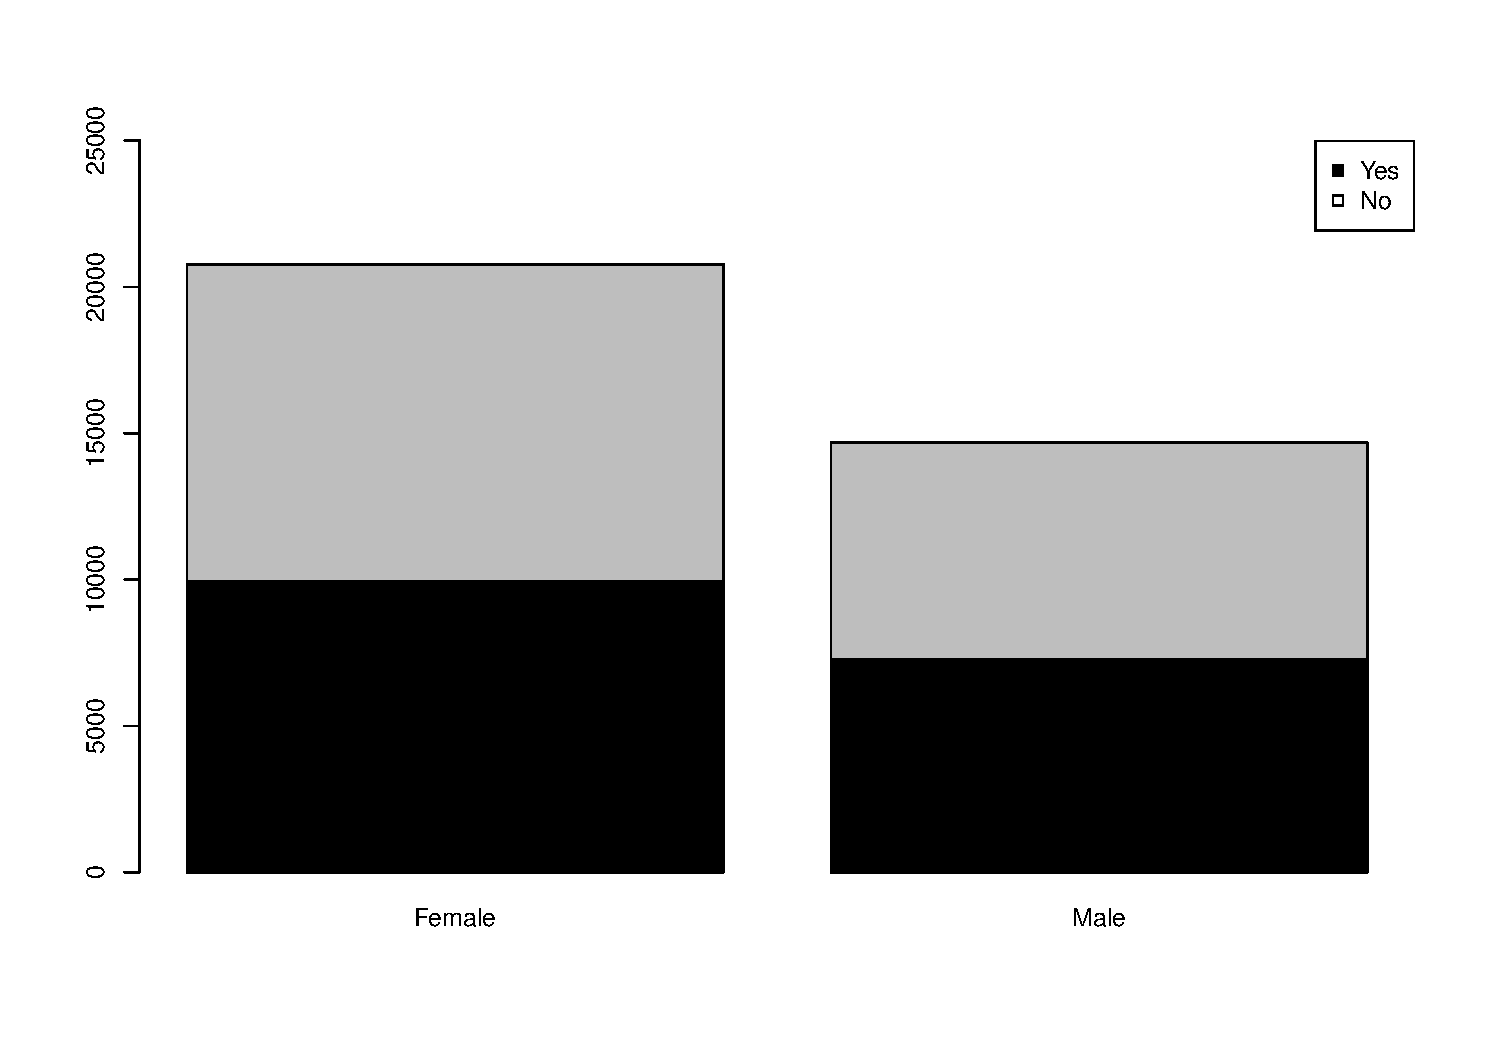
\includegraphics[width=\linewidth]{pic/enroll_gender}
\caption{} \label{enroll:a}
\end{subfigure}\hspace*{\fill}
\begin{subfigure}{0.48\textwidth }
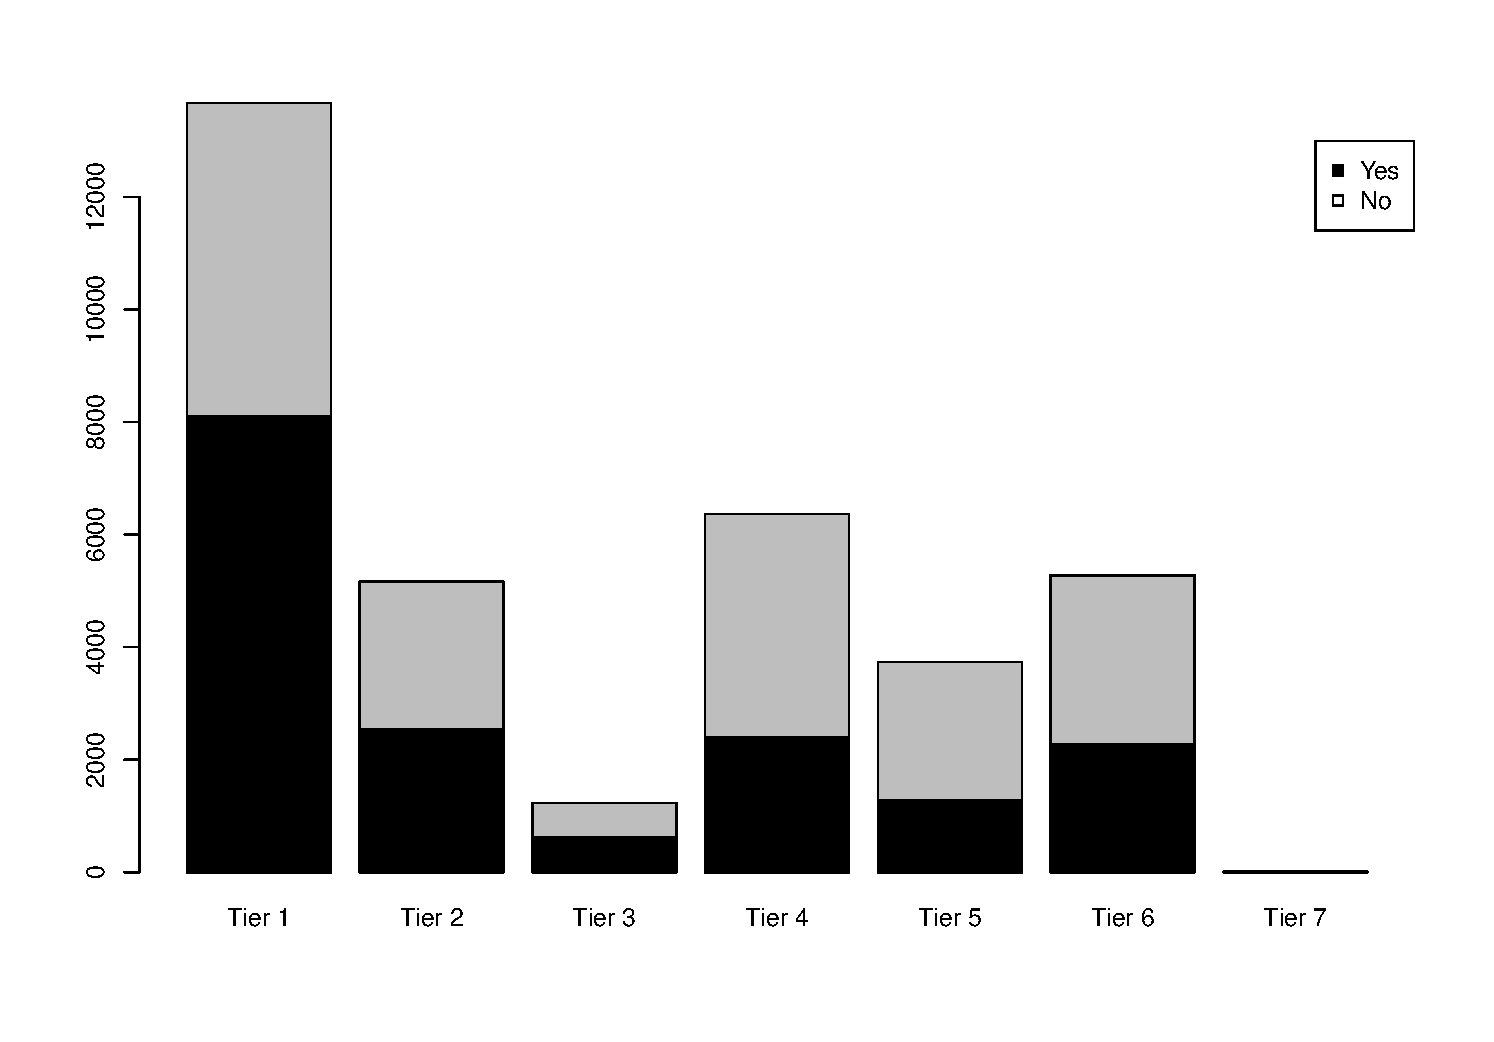
\includegraphics[width=\linewidth]{pic/enroll_tier}
\caption{} \label{enroll:b}
\end{subfigure}
\medskip
\begin{subfigure}{0.48\textwidth}
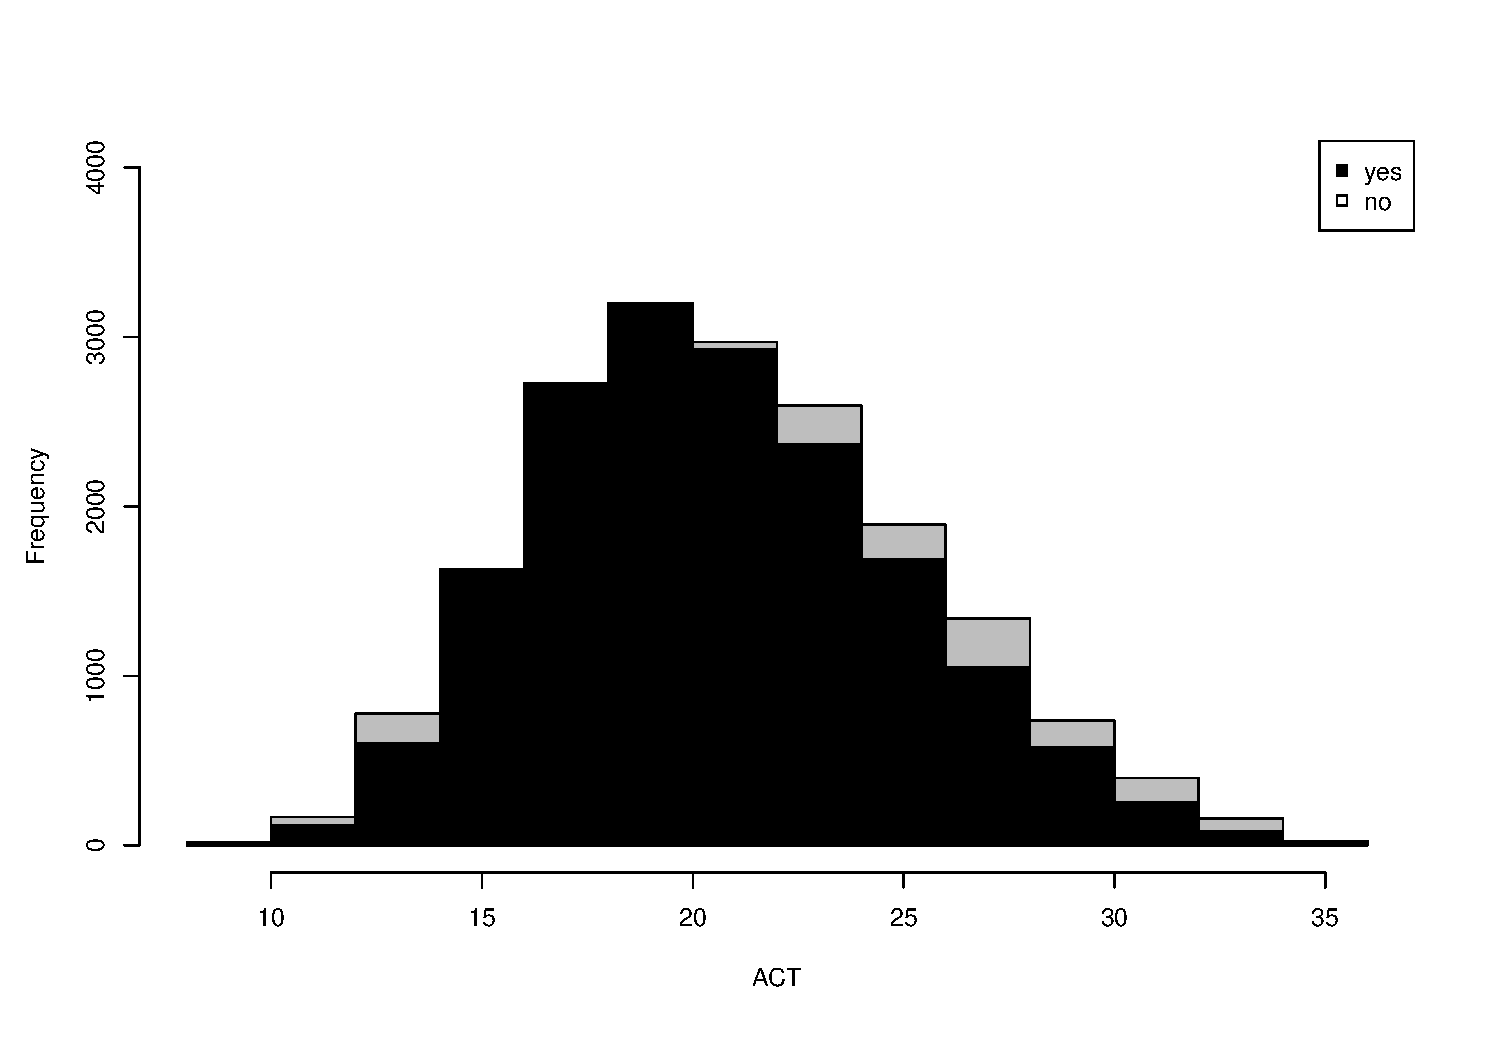
\includegraphics[width=\linewidth] {pic/enroll_act}
\caption{} \label{enroll:c}
\end{subfigure}\hspace*{\fill}
\begin{subfigure}{0.48\textwidth}
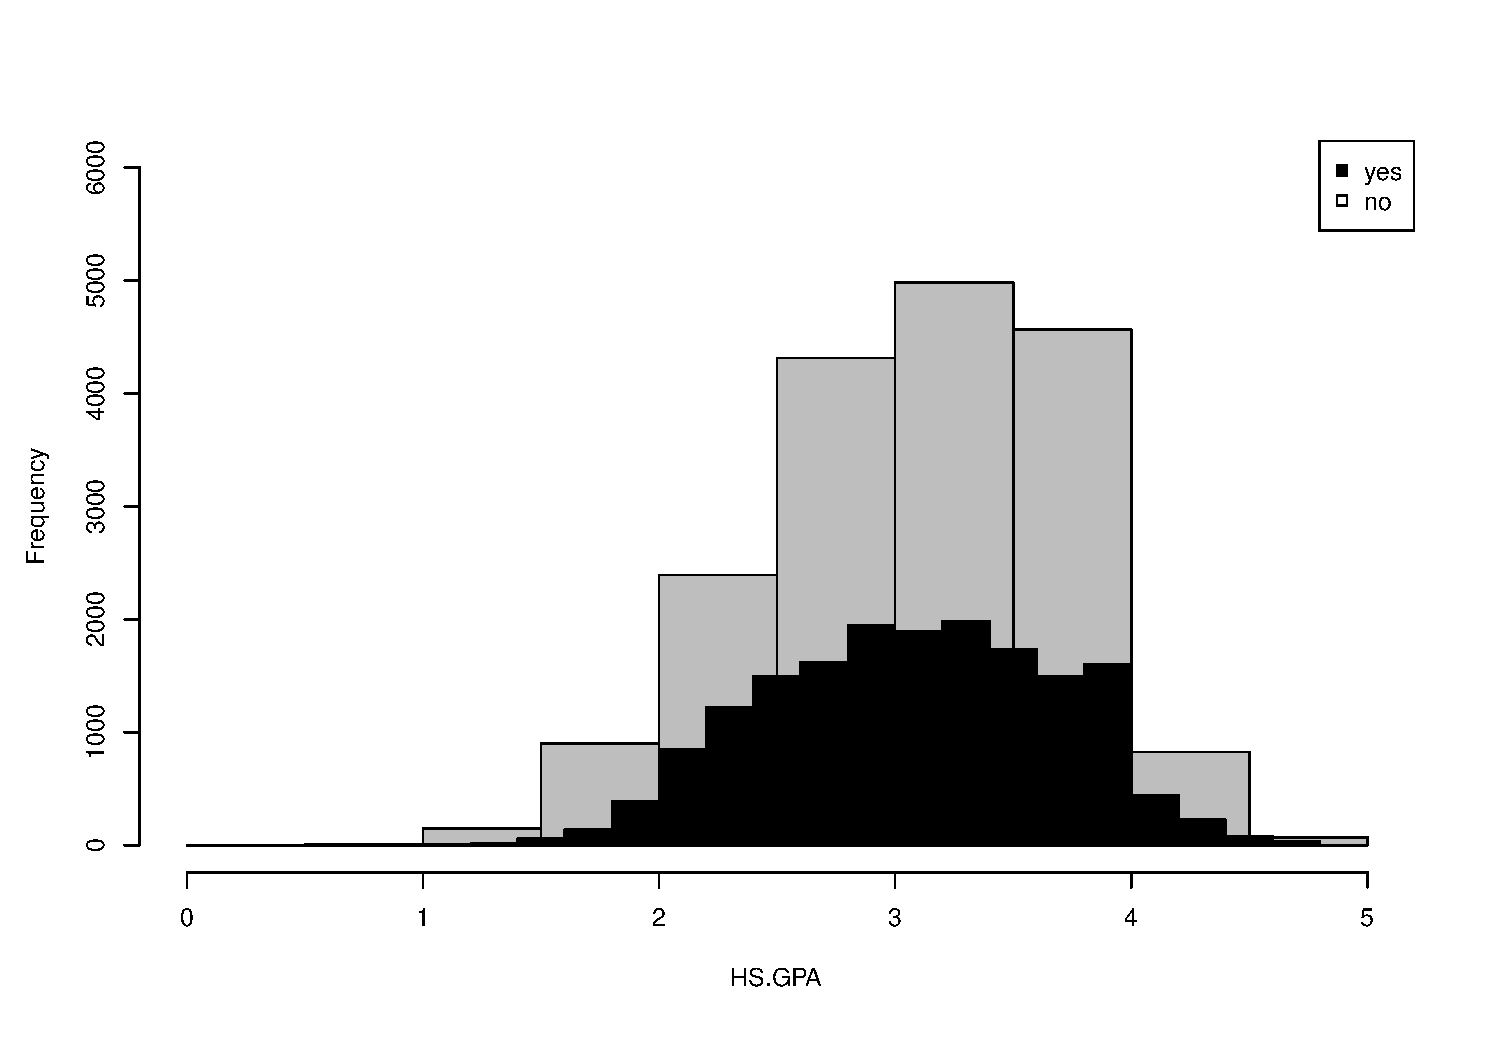
\includegraphics[width=\linewidth]{pic/enroll_gpa}
\caption{} \label{enroll:d}
\end{subfigure}

\medskip
\begin{subfigure}{0.45\textwidth}
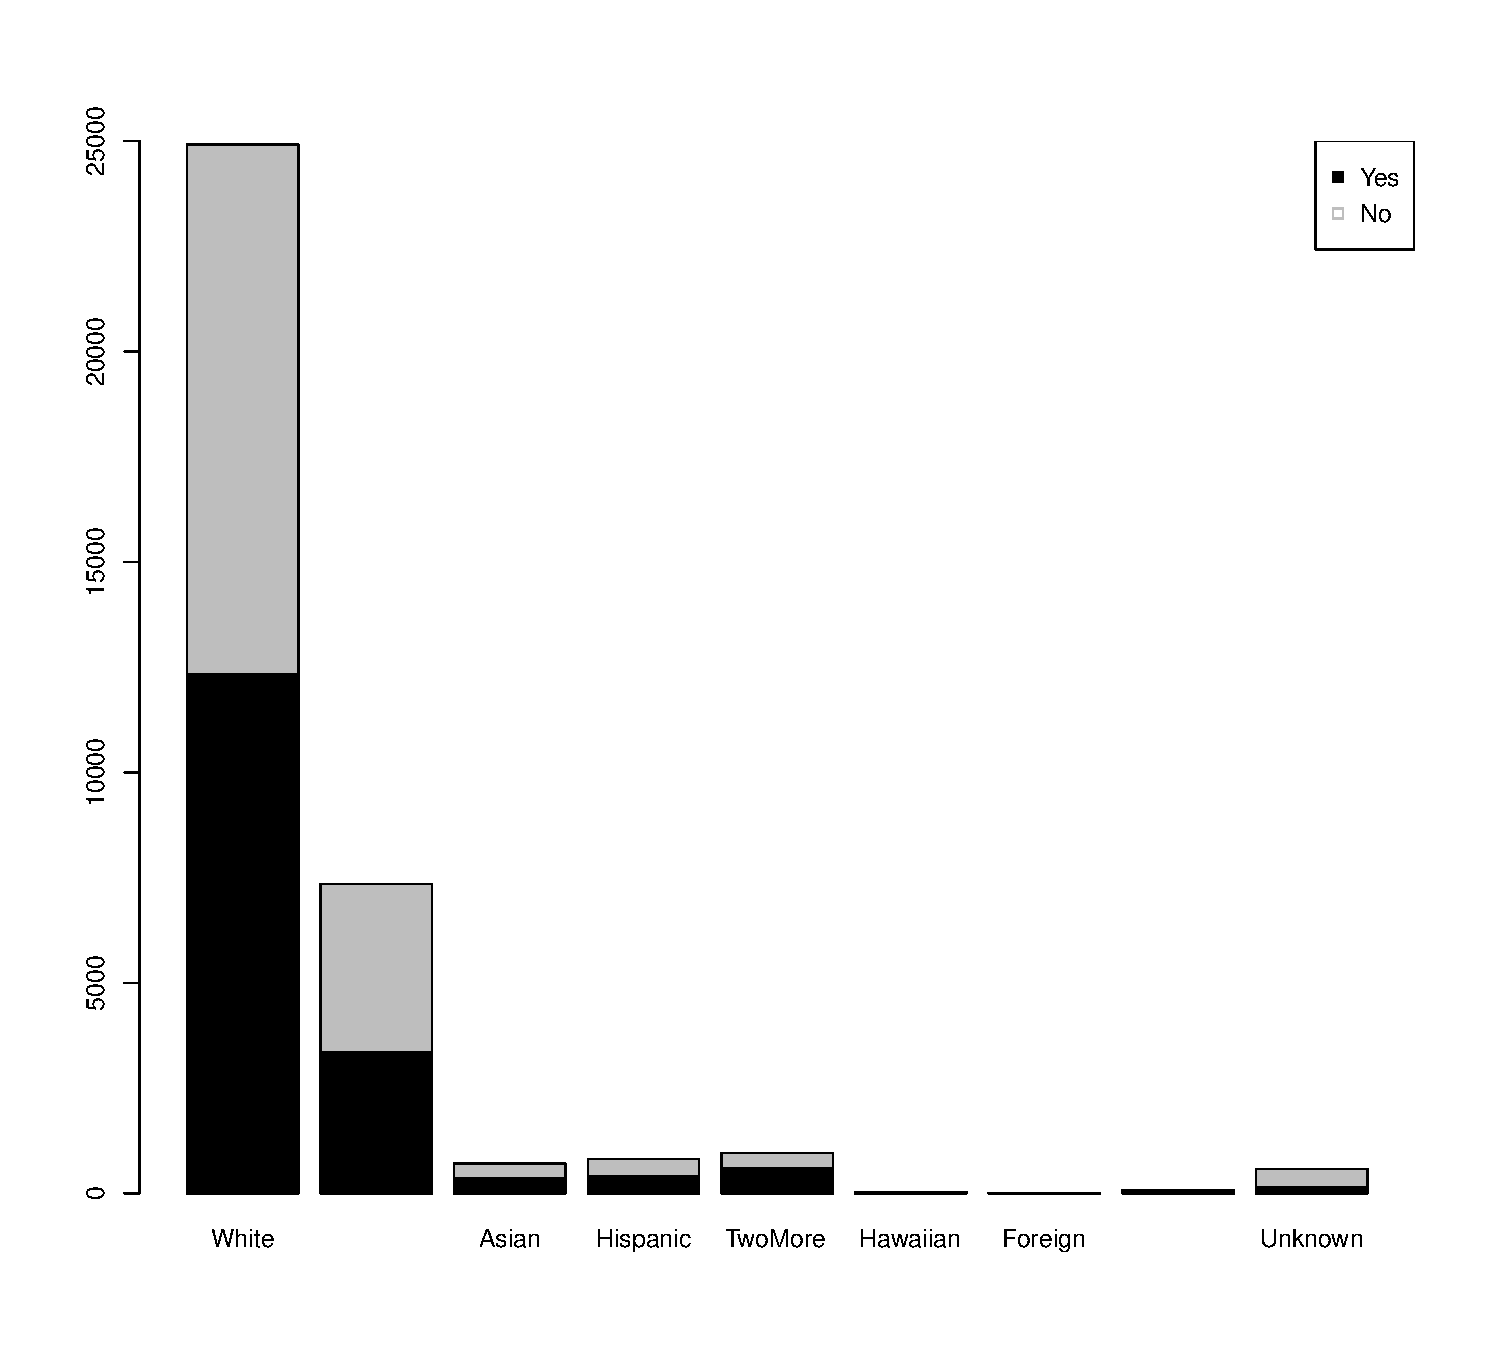
\includegraphics[width=\linewidth, height=6cm]{pic/enroll_ethnicity}
\caption{} \label{enroll:e}
\end{subfigure}\hspace*{\fill}
\begin{subfigure}{0.45\textwidth}
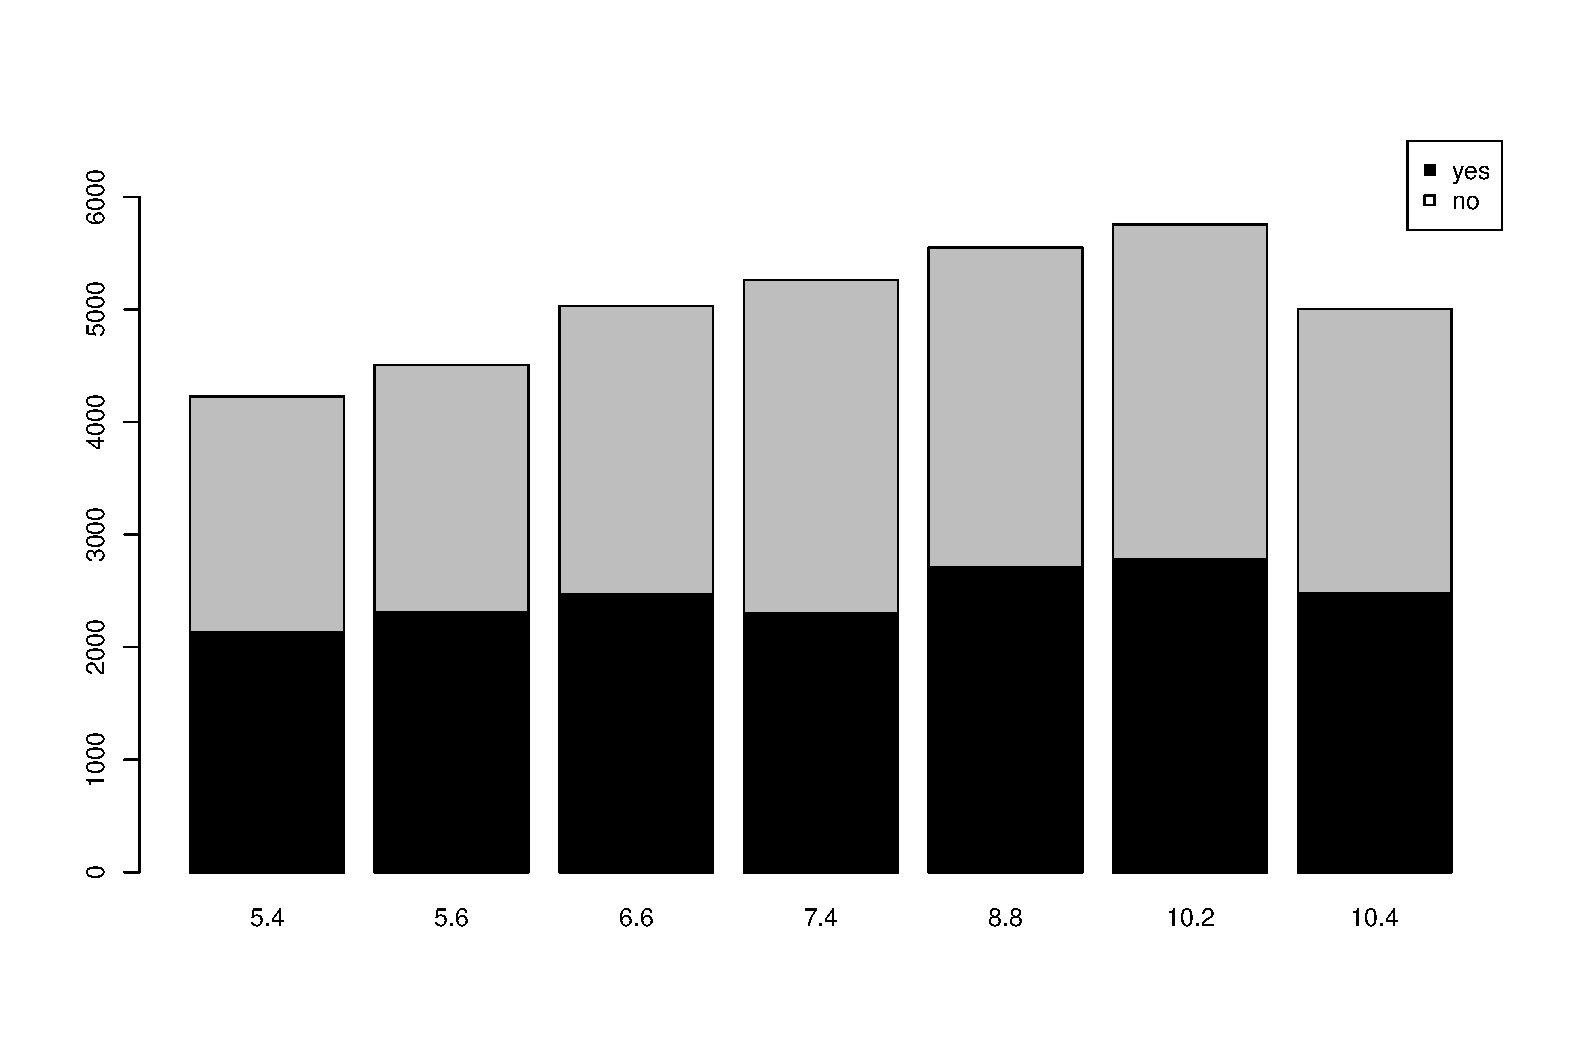
\includegraphics[width=\linewidth, height=6cm]{pic/enroll_index}
\caption{} \label{enroll:f}
\end{subfigure}
  \caption{Histogram plot for some important variables in enrollment
prediction: 
                        (a) Gender (b) Tier (c) ACT Score (d) High school GPA
(e) Ethnicity (f) Unemployment Index}
  \label{enroll_sum} 
\end{figure}





\begin{figure}[p]
\begin{subfigure}{0.48\textwidth}
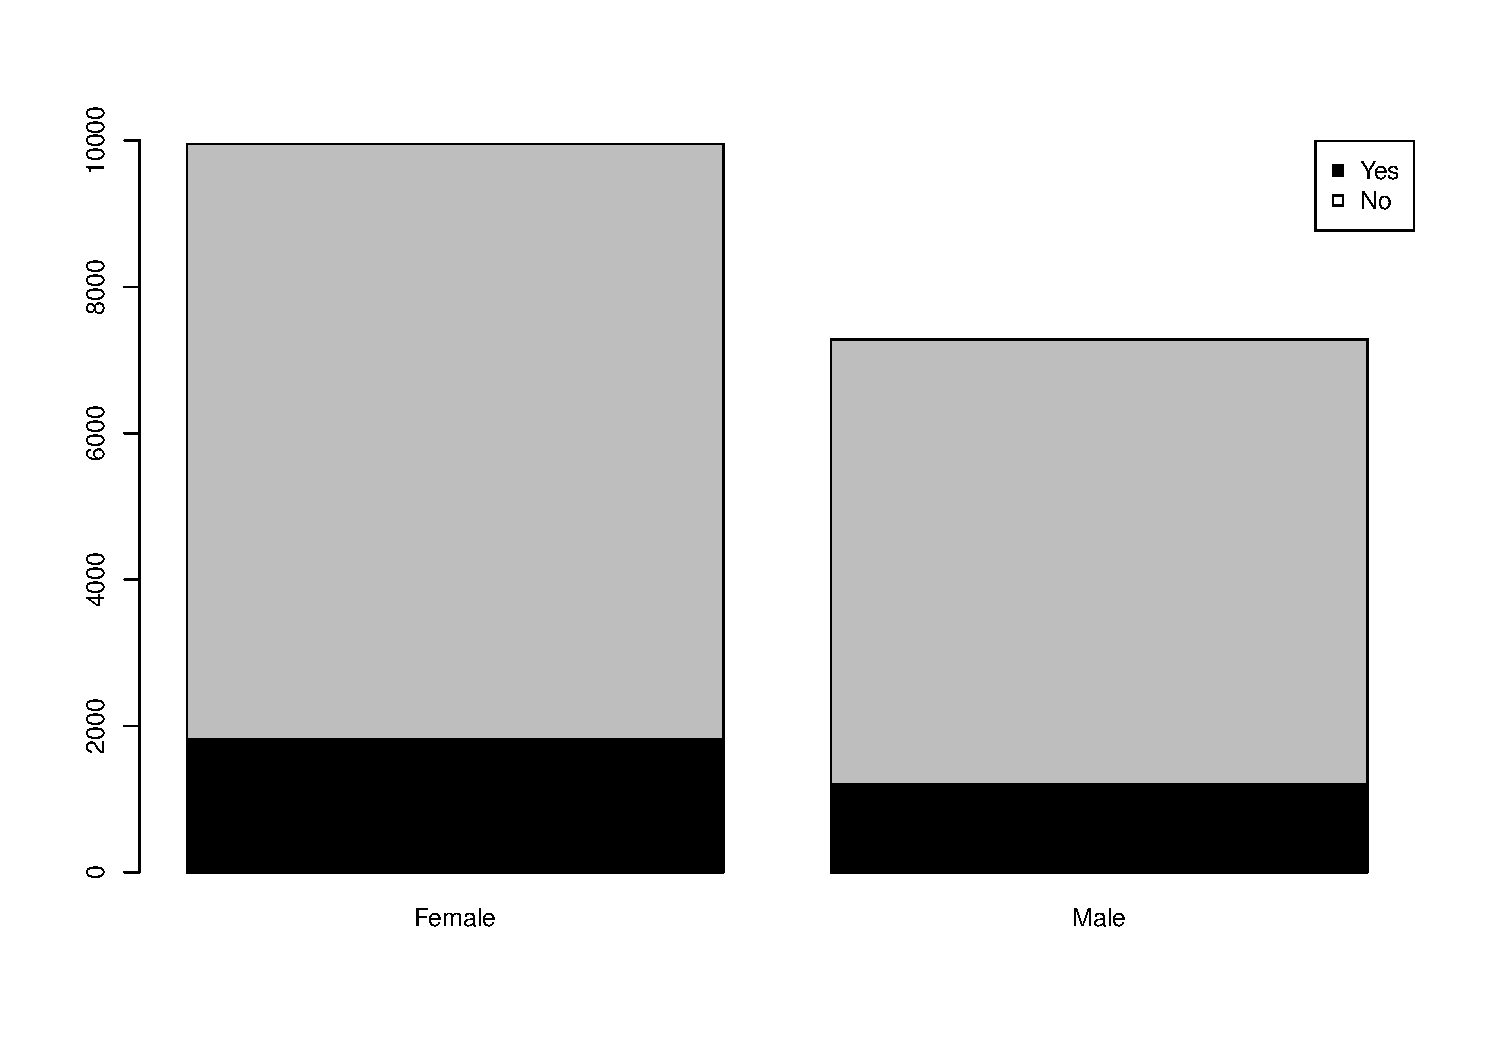
\includegraphics[width=\linewidth]{pic/grad_gender}
\caption{} \label{grad:a}
\end{subfigure}\hspace*{\fill}
\begin{subfigure}{0.48\textwidth}
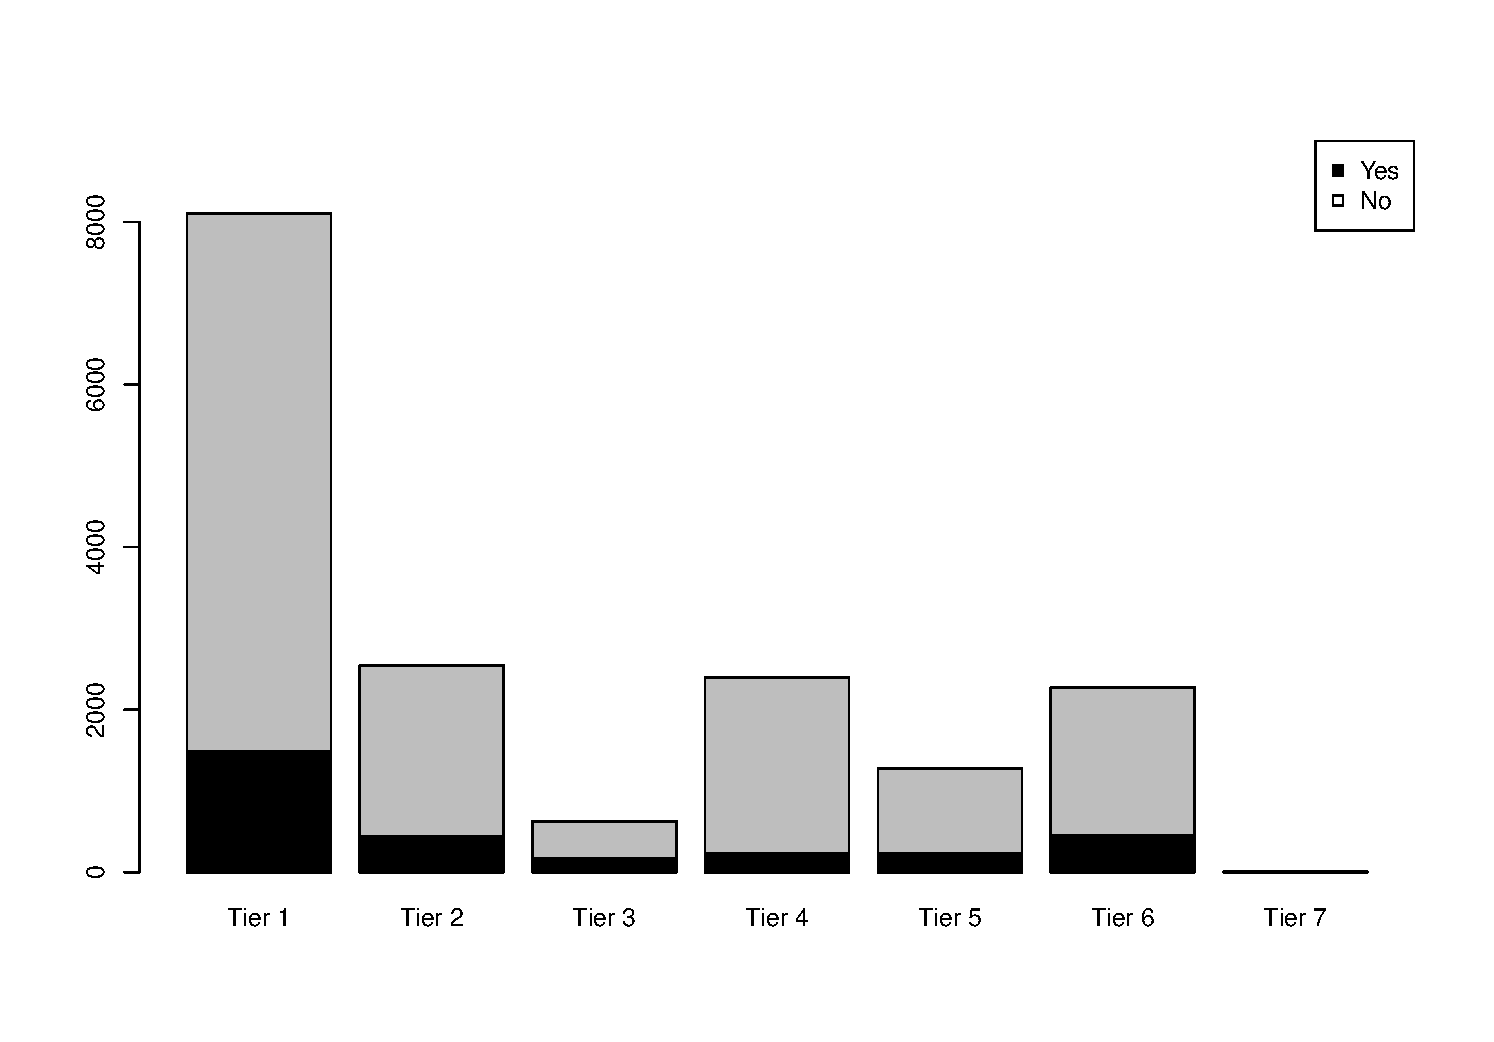
\includegraphics[width=\linewidth]{pic/grad_tier}
\caption{} \label{grad:b}
\end{subfigure}

\medskip
\begin{subfigure}{0.48\textwidth}
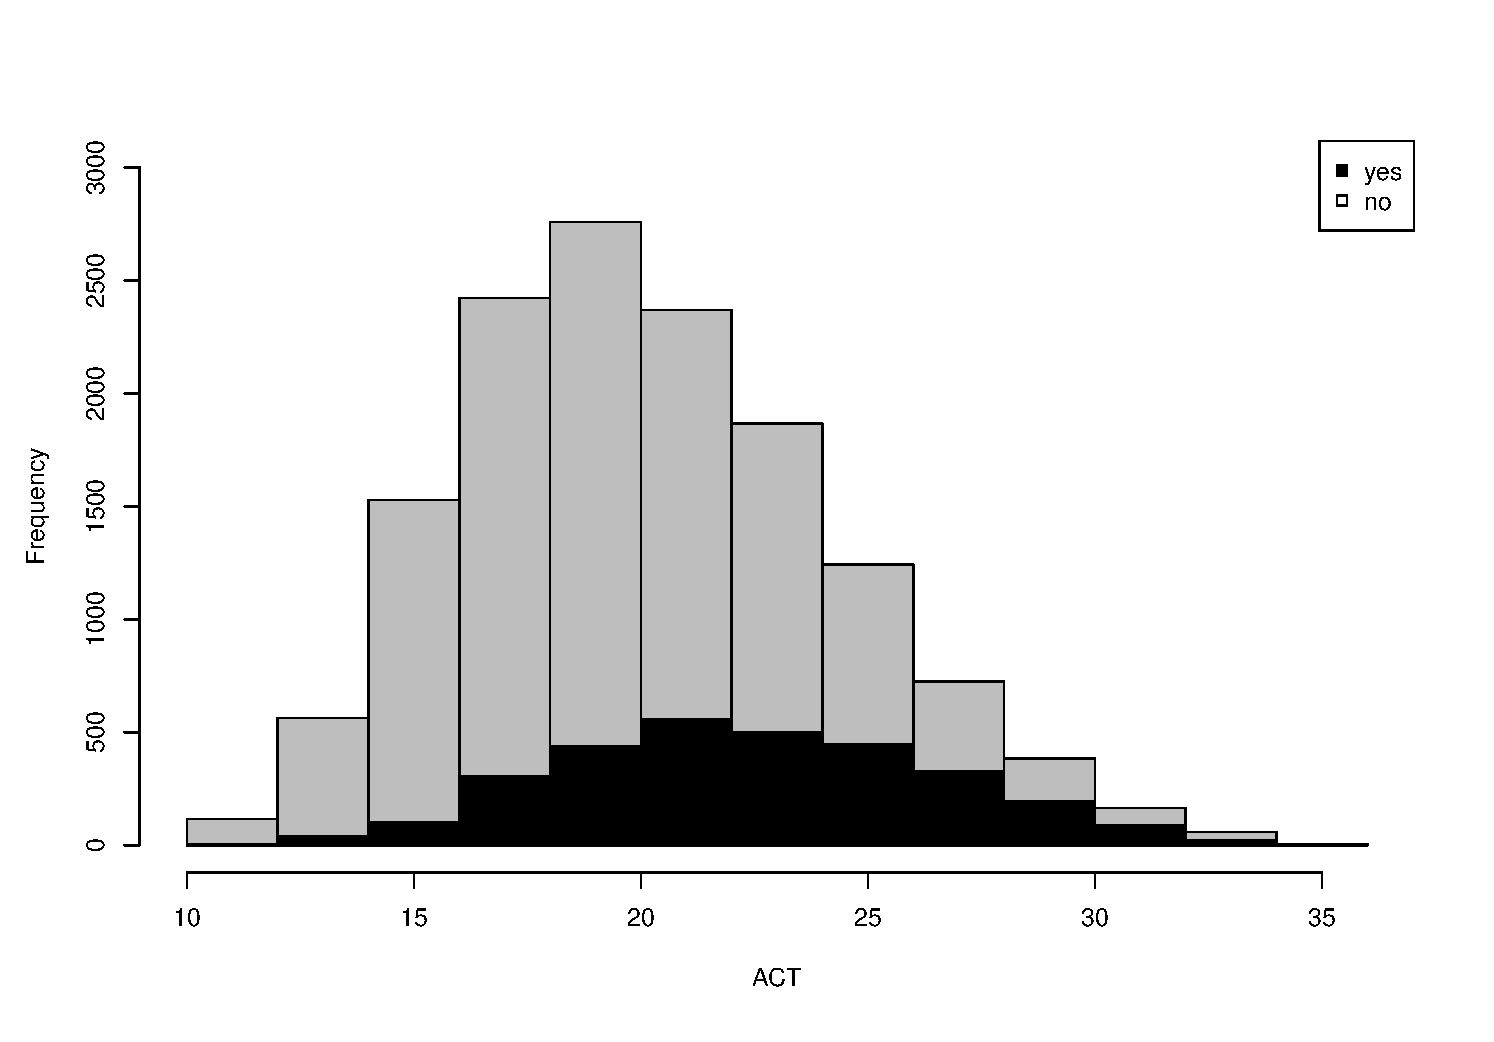
\includegraphics[width=\linewidth]{pic/grad_act}
\caption{} \label{grad:c}
\end{subfigure}\hspace*{\fill}
\begin{subfigure}{0.48\textwidth}
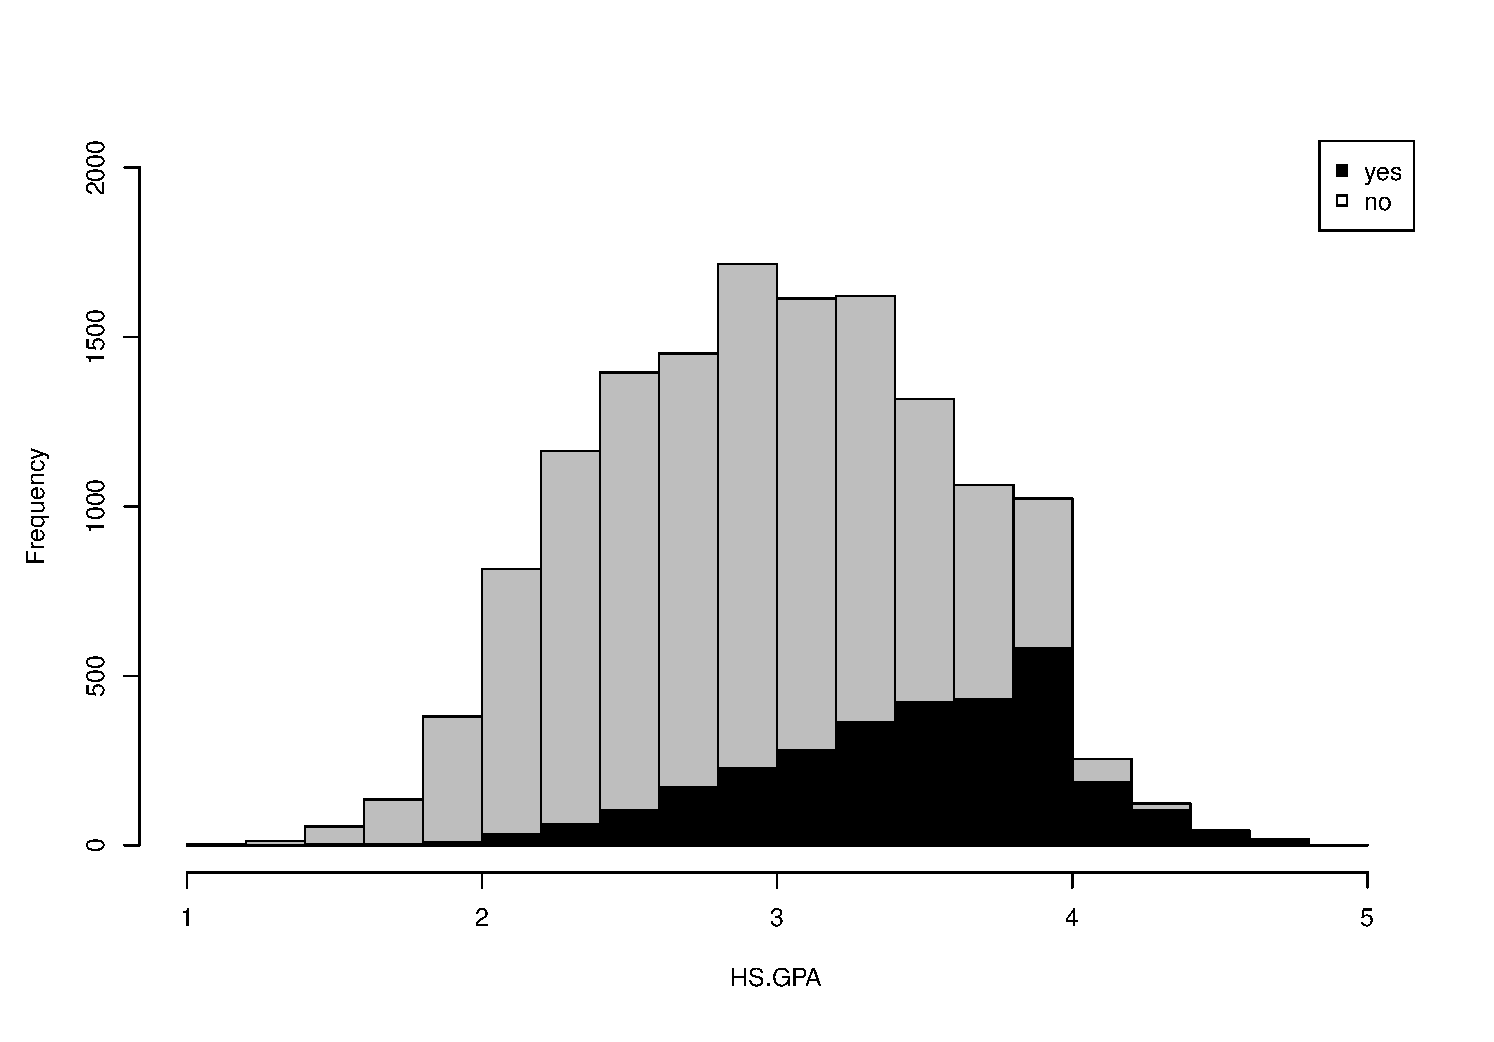
\includegraphics[width=\linewidth]{pic/grad_gpa}
\caption{} \label{grad:d}
\end{subfigure}

\medskip
\begin{subfigure}{0.48\textwidth}
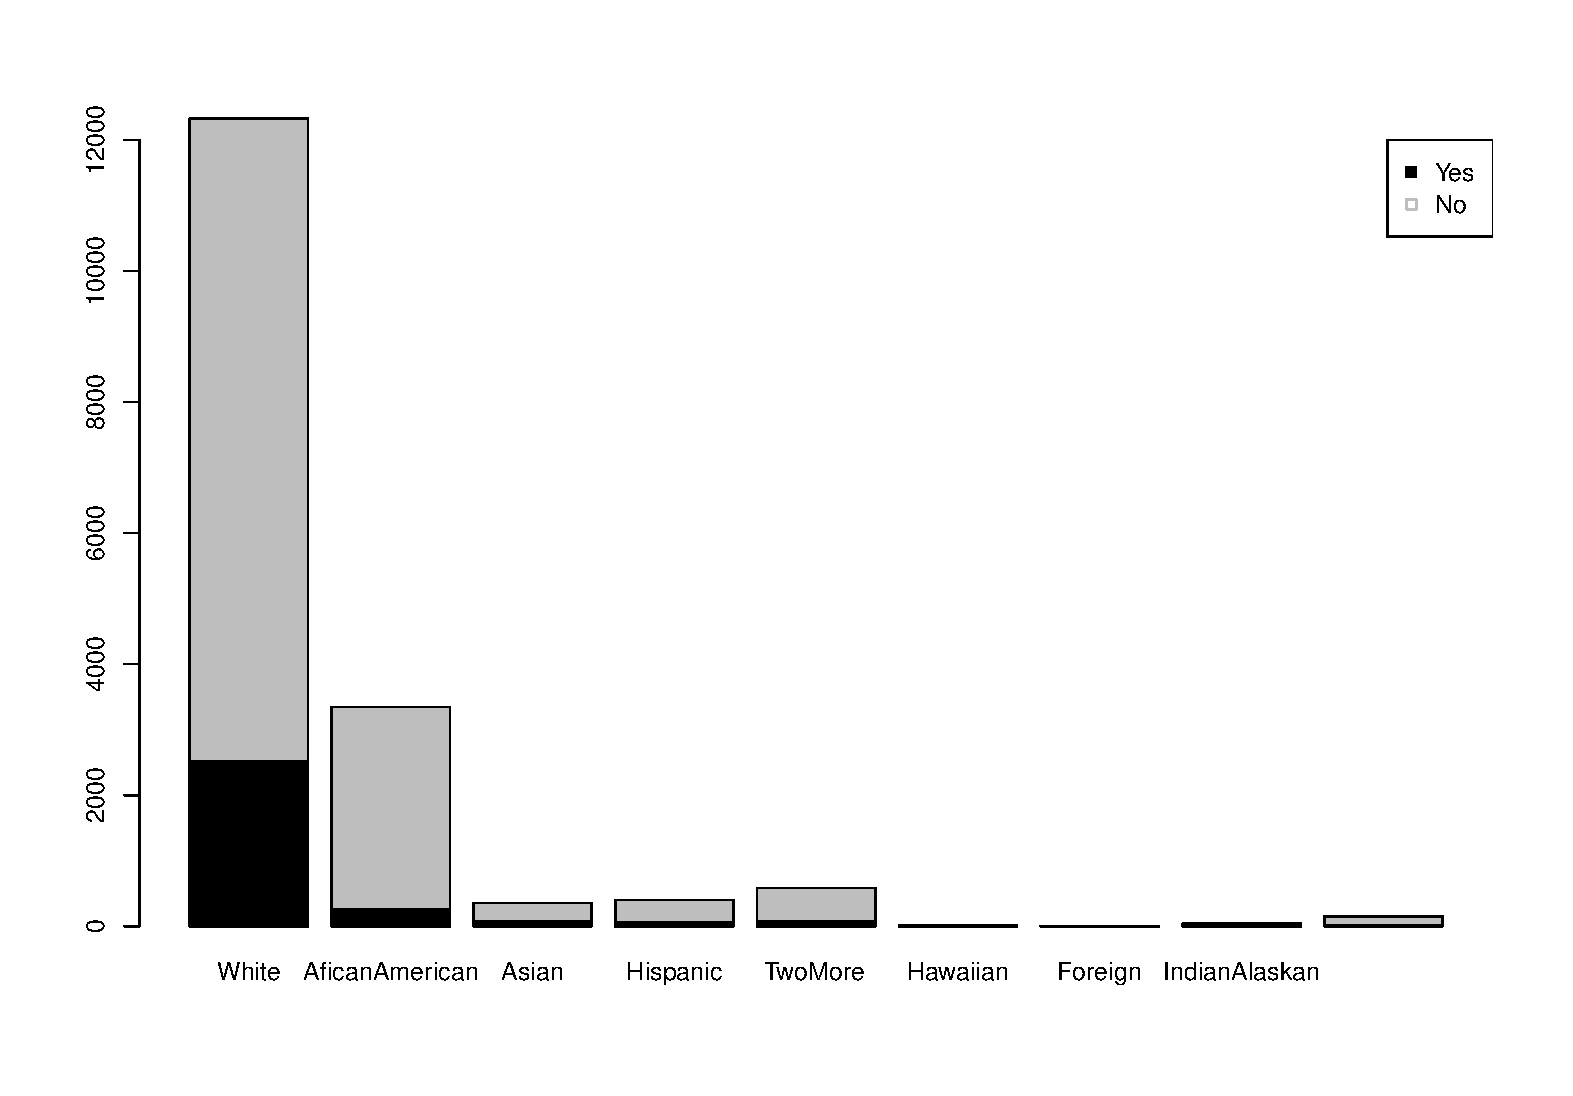
\includegraphics[width=\linewidth]{pic/grad_ethnicity}
\caption{} \label{grad:e}
\end{subfigure}\hspace*{\fill}
\begin{subfigure}{0.48\textwidth}
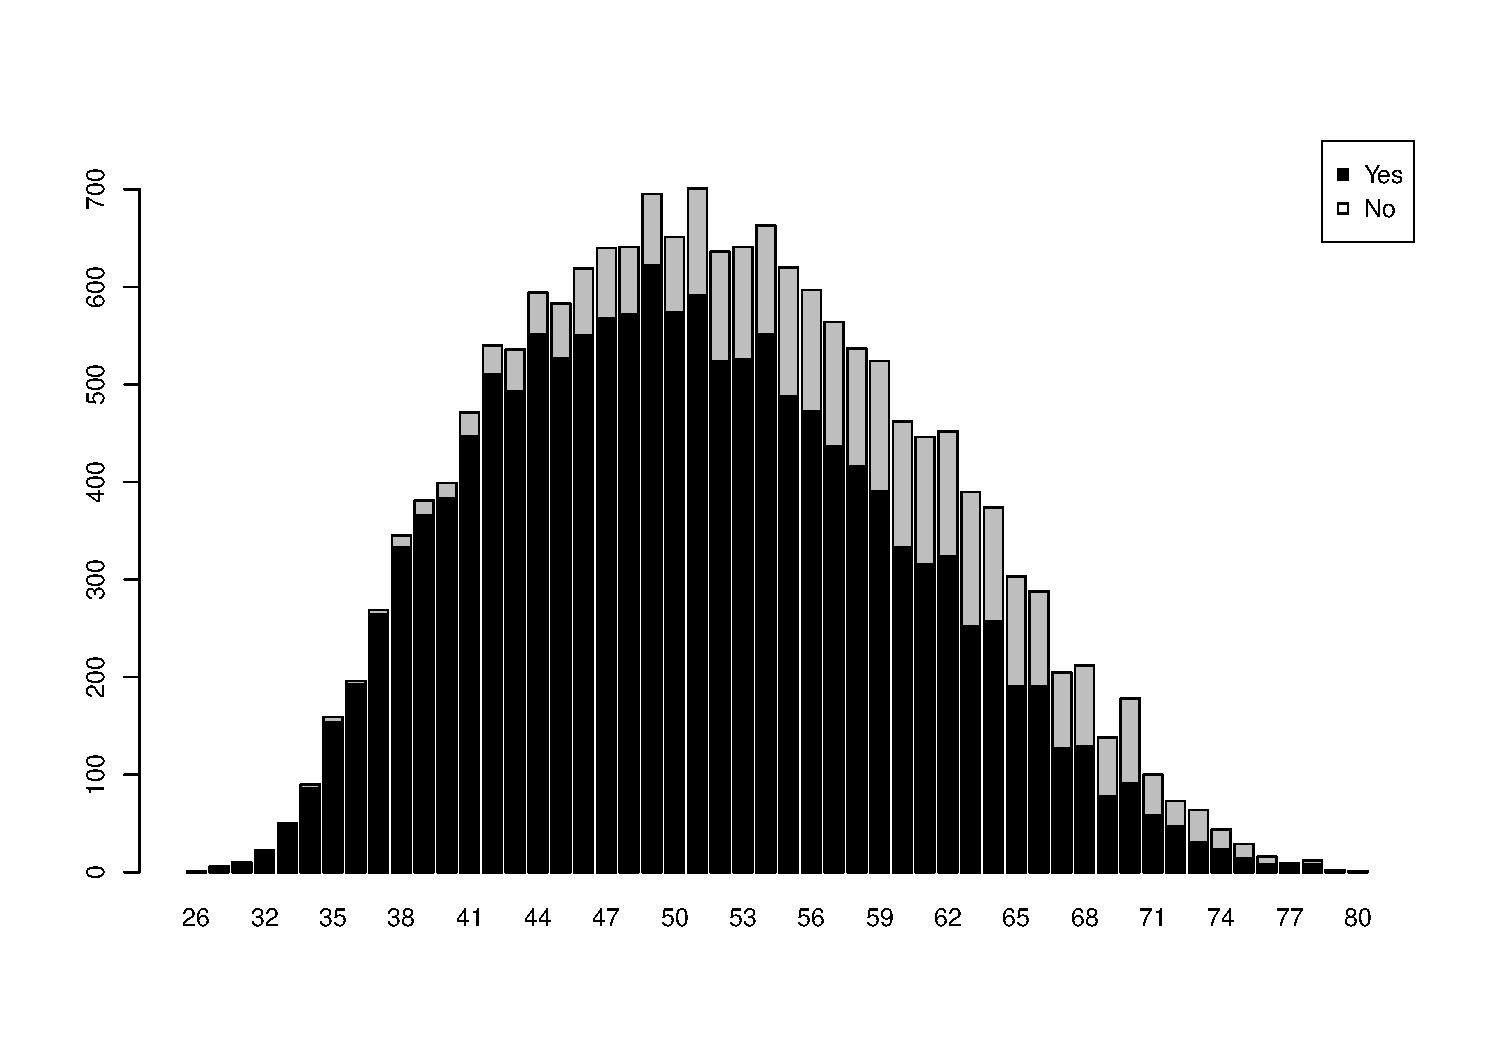
\includegraphics[width=\linewidth]{pic/grad_comp}
\caption{} \label{grad:f}
\end{subfigure}
  \caption{Histogram plot for some important variables in graduation
prediction: 
                        (a) Gender (b) Tier (c) ACT Score (d) High school GPA
(e) Ethnicity (f) Composite Score} 
  \label{grad_sum} 
\end{figure}



The data fields associated with these applications can be classified into
following categories: 1) academic performance related, 2) financial related,
and 3) personal information. The fields in academic related category includes
the applicant's SAT/ACT scores, GPA, and high school percentile; the  fields in
financial  related category includes family income, expected family
contribution (EFC), Pell grant; the fields in personal information category
includes gender, ethnicity, high school, intended college, and intended major.

In the academic performance related fields, to normalize, the ACT score was
translated into a percentile, for details on the mapping, please see
\citet{ACT_percentile}.
 
In the financial related fields or variables, expected family contribution
(EFC) measures an applicant's family's financial strength and is calculated
according to a formula established by law. The Federal Pell Grant is a
need-based grants to low-income students and is dependent on EFC. To better
estimate an applicant's affordability, two more variables are introduced: total
free money and out of pocket. The former defines all the awards that an
applicant gets while the latter is the total out\-of\-pocket money an applicant
pays.

In the personal information related field, to better estimate the distance
between applicants distance to the university, a variable was introduced that
represents the distance of the applicants' high school (a character variable)
into the distance from the high school to the university.

To get an idea of the application poll, an average students has a average GPA
of 3.0 and an average composite ACT score 21.2 (the state average composite ACT
score is 22.0, please see \citet{mean_sat}). 60\% of the applicants are female
and 40\% are male.  %The average effective family contribution is \$1400
    
To get a better picture of the applications distributions across academic
measure, Table \ref{num_act_gpa}) and the number of applicants in specific GPA
and ACT scores. To get a better picture of the applications distribution across
geographic regions, figure presents the number of applicants across the
geographic locations.

Finally, summary statistics of the variables are presented in Appendix \ref{app
A}.


\begin{sidewaystable}[!htbp]
 \resizebox{\linewidth}{200pt}{
\begin{tabular}{@{\extracolsep{5pt}}|c|ccccccccccccccccccccccccccc|c|}
\hline
GPA/ACT     & \multicolumn{1}{c|}{9} & \multicolumn{1}{c|}{10} &
\multicolumn{1}{c|}{11} & \multicolumn{1}{c|}{12} & \multicolumn{1}{c|}{13} &
\multicolumn{1}{c|}{14}  & \multicolumn{1}{c|}{15}  & \multicolumn{1}{c|}{16}
& \multicolumn{1}{c|}{17}  & \multicolumn{1}{c|}{18}  & \multicolumn{1}{c|}{19}
& \multicolumn{1}{c|}{20}  & \multicolumn{1}{c|}{21}  & \multicolumn{1}{c|}{22}
& \multicolumn{1}{c|}{23}  & \multicolumn{1}{c|}{24}  & \multicolumn{1}{c|}{25}
& \multicolumn{1}{c|}{26}  & \multicolumn{1}{c|}{27}  & \multicolumn{1}{c|}{28}
& \multicolumn{1}{c|}{29}  & \multicolumn{1}{c|}{30} & \multicolumn{1}{c|}{31}
& \multicolumn{1}{c|}{32} & \multicolumn{1}{c|}{33} & \multicolumn{1}{c|}{34} &
35 & Grand Total \\ \hline
1           &                        &                         &
&                         & 1                       &
& 2                        &                          &
&                          &                          &
&                          &                          &
&                          &                          &
&                          &                          &
&                         &                         &                         &
&                         &    & 3           \\ \cline{1-1} \cline{29-29}
1.1         &                        &                         &
&                         &                         &
&                          &                          & 1
&                          &                          &
&                          &                          &
&                          &                          &
&                          &                          &
&                         &                         &                         &
&                         &    & 1           \\ \cline{1-1} \cline{29-29}
1.2         &                        &                         &
&                         & 1                       &
&                          &                          &
&                          & 1                        &
&                          &                          &
&                          &                          &
&                          &                          &
&                         &                         &                         &
&                         &    & 2           \\ \cline{1-1} \cline{29-29}
1.3         &                        &                         &
& 1                       &                         &
&                          & 1                        &
& 1                        &                          &
&                          &                          &
&                          &                          &
&                          &                          &
&                         &                         &                         &
&                         &    & 3           \\ \cline{1-1} \cline{29-29}
1.4         &                        &                         &
& 1                       &                         & 2
&                          & 1                        &
&                          & 2                        &
&                          &                          &
&                          &                          &
&                          &                          &
&                         &                         &                         &
&                         &    & 6           \\ \cline{1-1} \cline{29-29}
1.5         &                        &                         &
& 1                       & 2                       & 2
& 1                        & 6                        & 3
&                          & 3                        &
&                          &                          &
&                          &                          & 1
&                          &                          &
&                         &                         &                         &
&                         &    & 19          \\ \cline{1-1} \cline{29-29}
1.6         &                        &                         &
& 1                       & 4                       & 4
& 2                        & 4                        & 4
& 4                        & 2                        & 3
& 2                        & 2                        & 1
& 1                        &                          &
&                          &                          &
&                         &                         &                         &
&                         &    & 34          \\ \cline{1-1} \cline{29-29}
1.7         & 1                      &                         &
& 2                       & 5                       & 4
& 7                        & 3                        & 2
& 5                        & 6                        & 1
& 1                        & 2                        & 1
& 2                        & 2                        & 1
&                          &                          &
&                         &                         &                         &
&                         &    & 45          \\ \cline{1-1} \cline{29-29}
1.8         &                        &                         &
&                         & 4                       & 8
& 5                        & 9                        & 4
& 8                        & 4                        & 1
& 1                        & 1                        &
&                          &                          &
&                          &                          &
&                         &                         &                         &
&                         &    & 45          \\ \cline{1-1} \cline{29-29}
1.9         &                        & 1                       & 1
& 2                       & 1                       & 11
& 9                        & 7                        & 9
& 5                        & 5                        & 5
& 4                        & 3                        & 3
&                          & 2                        &
&                          &                          &
&                         &                         &                         &
&                         &    & 68          \\ \cline{1-1} \cline{29-29}
2           &                        &                         &
& 2                       & 4                       & 5
& 7                        & 14                       & 9
& 10                       & 7                        & 7
& 4                        & 6                        & 3
& 1                        & 1                        &
&                          &                          & 1
&                         &                         &                         &
&                         &    & 81          \\ \cline{1-1} \cline{29-29}
2.1         & 1                      &                         &
& 5                       & 8                       & 7
& 17                       & 23                       & 8
& 14                       & 12                       & 7
& 5                        & 5                        & 2
&                          & 1                        & 1
& 1                        &                          &
& 1                       &                         &                         &
&                         &    & 118         \\ \cline{1-1} \cline{29-29}
2.2         &                        &                         & 1
& 3                       & 7                       & 7
& 11                       & 12                       & 23
& 18                       & 13                       & 13
& 8                        & 5                        & 2
& 7                        & 2                        & 2
& 1                        & 1                        & 1
&                         &                         &                         &
&                         &    & 137         \\ \cline{1-1} \cline{29-29}
2.3         &                        &                         & 1
& 3                       & 5                       & 9
& 21                       & 21                       & 29
& 19                       & 17                       & 15
& 13                       & 5                        & 5
& 7                        & 2                        & 3
& 1                        & 2                        &
&                         &                         &                         &
&                         &    & 178         \\ \cline{1-1} \cline{29-29}
2.4         &                        &                         &
& 1                       & 4                       & 13
& 20                       & 17                       & 30
& 15                       & 16                       & 19
& 21                       & 7                        & 8
& 5                        & 2                        & 3
& 2                        &                          &
& 1                       &                         &                         &
&                         &    & 184         \\ \cline{1-1} \cline{29-29}
2.5         &                        &                         &
& 4                       & 3                       & 13
& 17                       & 26                       & 26
& 22                       & 29                       & 17
& 18                       & 11                       & 7
& 8                        & 3                        & 3
& 1                        & 1                        & 2
&                         & 1                       &                         &
&                         &    & 212         \\ \cline{1-1} \cline{29-29}
2.6         &                        &                         & 1
& 3                       & 4                       & 10
& 10                       & 21                       & 26
& 38                       & 28                       & 15
& 13                       & 5                        & 13
& 11                       & 5                        & 2
& 4                        &                          & 2
& 1                       &                         &                         &
1                       &                         &    & 213         \\
\cline{1-1} \cline{29-29}
2.7         &                        &                         & 3
&                         & 2                       & 7
& 17                       & 22                       & 32
& 27                       & 33                       & 23
& 15                       & 15                       & 15
& 7                        & 3                        & 2
& 1                        & 1                        &
& 2                       &                         &                         &
&                         &    & 227         \\ \cline{1-1} \cline{29-29}
2.8         &                        &                         &
& 2                       & 4                       & 7
& 12                       & 10                       & 28
& 27                       & 29                       & 23
& 19                       & 20                       & 14
& 13                       & 4                        & 7
& 5                        & 2                        & 1
&                         &                         &                         &
1                       &                         &    & 228         \\
\cline{1-1} \cline{29-29}
2.9         &                        &                         & 1
& 2                       & 7                       & 9
& 11                       & 25                       & 21
& 39                       & 32                       & 40
& 20                       & 22                       & 20
& 15                       & 12                       & 11
& 4                        & 1                        &
&                         &                         &                         &
&                         &    & 292         \\ \cline{1-1} \cline{29-29}
3           &                        &                         &
& 1                       & 1                       & 9
& 9                        & 16                       & 26
& 34                       & 33                       & 35
& 28                       & 28                       & 26
& 17                       & 15                       & 10
& 3                        & 2                        & 5
&                         & 2                       &                         &
& 1                       &    & 301         \\ \cline{1-1} \cline{29-29}
3.1         &                        &                         &
& 3                       & 2                       & 6
& 12                       & 11                       & 18
& 36                       & 35                       & 39
& 38                       & 18                       & 24
& 21                       & 15                       & 11
& 4                        & 4                        & 2
& 1                       &                         &                         &
&                         & 1  & 301         \\ \cline{1-1} \cline{29-29}
3.2         &                        &                         &
&                         &                         & 6
& 7                        & 17                       & 19
& 26                       & 26                       & 32
& 29                       & 37                       & 32
& 16                       & 16                       & 8
& 12                       & 3                        & 8
& 5                       & 4                       & 1                       &
&                         &    & 304         \\ \cline{1-1} \cline{29-29}
3.3         &                        &                         & 1
&                         & 1                       & 4
& 8                        & 5                        & 23
& 22                       & 31                       & 33
& 22                       & 34                       & 27
& 22                       & 27                       & 19
& 13                       & 10                       & 4
& 3                       & 5                       &                         &
1                       & 2                       &    & 317         \\
\cline{1-1} \cline{29-29}
3.4         &                        & 1                       &
&                         & 1                       &
& 3                        & 9                        & 9
& 14                       & 21                       & 31
& 36                       & 35                       & 30
& 26                       & 21                       & 16
& 10                       & 8                        & 5
& 2                       & 3                       &                         &
&                         &    & 281         \\ \cline{1-1} \cline{29-29}
3.5         &                        &                         &
&                         &                         &
& 5                        & 5                        & 8
& 13                       & 16                       & 23
& 27                       & 29                       & 25
& 29                       & 30                       & 22
& 14                       & 11                       & 5
& 7                       & 2                       &                         &
1                       &                         &    & 272         \\
\cline{1-1} \cline{29-29}
3.6         &                        &                         &
&                         &                         &
& 2                        & 3                        & 4
& 3                        & 22                       & 17
& 21                       & 30                       & 37
& 28                       & 23                       & 25
& 18                       & 11                       & 10
& 6                       & 1                       & 3                       &
2                       & 2                       &    & 268         \\
\cline{1-1} \cline{29-29}
3.7         &                        &                         &
&                         &                         & 2
& 1                        &                          & 3
& 7                        & 12                       & 10
& 20                       & 20                       & 28
& 28                       & 22                       & 25
& 23                       & 16                       & 13
& 5                       & 2                       & 2                       &
& 2                       &    & 241         \\ \cline{1-1} \cline{29-29}
3.8         &                        &                         &
&                         &                         &
& 2                        &                          &
& 3                        & 8                        & 13
& 13                       & 20                       & 18
& 29                       & 19                       & 18
& 27                       & 15                       & 11
& 10                      & 3                       & 2                       &
2                       &                         &    & 213         \\
\cline{1-1} \cline{29-29}
3.9         &                        &                         &
&                         &                         &
& 1                        & 2                        & 2
& 3                        & 6                        & 6
& 8                        & 14                       & 24
& 26                       & 19                       & 25
& 19                       & 17                       & 18
& 11                      & 7                       & 5                       &
3                       & 1                       &    & 217         \\
\cline{1-1} \cline{29-29}
4           &                        &                         &
&                         &                         &
&                          & 1                        &
&                          & 2                        & 7
& 7                        & 7                        & 20
& 18                       & 19                       & 23
& 23                       & 21                       & 20
& 22                      & 9                       & 11                      &
12                      & 7                       & 2  & 231         \\
\cline{1-1} \cline{29-29}
4.1         &                        &                         &
&                         &                         &
&                          &                          & 1
&                          & 2                        & 2
& 1                        & 3                        & 7
& 8                        & 4                        & 6
& 9                        & 4                        & 4
& 6                       & 4                       & 2                       &
3                       & 1                       &    & 67          \\
\cline{1-1} \cline{29-29}
4.2         &                        &                         &
&                         &                         &
&                          &                          &
& 1                        &                          & 1
& 2                        & 4                        & 1
& 3                        & 5                        & 5
& 7                        & 3                        & 4
& 3                       & 2                       & 5                       &
1                       & 1                       &    & 48          \\
\cline{1-1} \cline{29-29}
4.3         &                        &                         &
&                         &                         &
&                          &                          &
&                          &                          &
&                          & 1                        & 2
& 4                        & 3                        & 2
& 2                        & 8                        & 3
& 3                       & 4                       & 4                       &
1                       & 1                       &    & 38          \\
\cline{1-1} \cline{29-29}
4.4         &                        &                         &
&                         &                         &
&                          &                          &
&                          &                          &
&                          &                          &
& 1                        & 4                        & 2
& 3                        & 1                        & 1
& 5                       & 2                       & 2                       &
1                       & 2                       &    & 24          \\
\cline{1-1} \cline{29-29}
4.5         &                        &                         &
&                         &                         &
&                          &                          &
&                          &                          & 1
&                          & 1                        & 4
&                          & 1                        & 1
&                          & 1                        & 3
&                         & 1                       & 2                       &
3                       &                         & 1  & 19          \\
\cline{1-1} \cline{29-29}
4.6         &                        &                         &
&                         &                         &
&                          &                          &
&                          &                          &
&                          &                          & 1
&                          &                          & 1
& 1                        & 1                        &
& 1                       &                         & 3                       &
1                       & 1                       &    & 10          \\
\cline{1-1} \cline{29-29}
4.7         &                        &                         &
&                         &                         &
&                          &                          &
&                          &                          &
& 1                        &                          &
&                          &                          & 1
& 3                        & 1                        &
&                         & 1                       & 1                       &
1                       &                         &    & 9           \\
\cline{1-1} \cline{29-29}
4.8         &                        &                         &
&                         &                         &
&                          &                          &
&                          &                          &
&                          &                          &
&                          &                          &
& 1                        & 1                        &
& 1                       &                         &                         &
&                         &    & 3           \\ \hline
Grand Total & \multicolumn{1}{c|}{2} & \multicolumn{1}{c|}{2}  &
\multicolumn{1}{c|}{9}  & \multicolumn{1}{c|}{37} & \multicolumn{1}{c|}{71} &
\multicolumn{1}{c|}{145} & \multicolumn{1}{c|}{219} & \multicolumn{1}{c|}{291}
& \multicolumn{1}{c|}{368} & \multicolumn{1}{c|}{414} &
\multicolumn{1}{c|}{453} & \multicolumn{1}{c|}{439} & \multicolumn{1}{c|}{397}
& \multicolumn{1}{c|}{390} & \multicolumn{1}{c|}{400} &
\multicolumn{1}{c|}{353} & \multicolumn{1}{c|}{282} & \multicolumn{1}{c|}{256}
& \multicolumn{1}{c|}{212} & \multicolumn{1}{c|}{146} &
\multicolumn{1}{c|}{123} & \multicolumn{1}{c|}{96} & \multicolumn{1}{c|}{53} &
\multicolumn{1}{c|}{43} & \multicolumn{1}{c|}{34} & \multicolumn{1}{c|}{21} & 4
& 5260        \\ \hline
\end{tabular}}
\caption{Number of Applicants vs GPA/ACT in 2012-2013}
\label{num_act_gpa}
\end{sidewaystable}

%  cost of attendance; the student's enrollment status; and whether the student
attends for a full academic year or less. The Federal Pell Grant data used in
the study was derived follow by \citep{EFC_Pell}.

\section{Logistic Regression Models}
Logistic regression is a popular method when predicting a dichotomous outcome
variable. In the case of prediction of enrollment, the response variable has
two levels (yes and no). The output of logistic regression model is the
probability of the enrollment levels; for example, a probability of 70\% of
enrollment (yes) for an applicant with GPA 2.5, ACT 28, given say a \$1000
scholarships.

Because of the fact that the probability of enrollment $p(x)$ must fall in
$[0,1]$, a regular linear regression is unsuitable as the regression function
is not bounded. To resolve this issue, the ratio, called the odds of success,
defined as  $\frac{p(x)}{1-p(x)}$,  is used to form a regression and and a
logistic function is defined as:
\begin{equation}
\ensuremath{\log\frac{p(x)}{1-p(x)}=\beta_0+\beta_1 x_1+\beta_2 x_2
+\ldots+\beta_k x_k}
\end{equation}
The probability of enrollment can thus be rewritten as:
\begin{equation}
p(x)=\frac{e^{\beta_0+\beta_1 x_1+\beta_2 x_2 +\ldots+\beta_i
x_i}}{1+e^{\beta_0+\beta_1 x_1+\beta_2 x_2 +\ldots+\beta_i
x_i}}%=\frac{1}{1+e^{-(\beta_0+\beta_0+\beta_1 x_1+\beta_2 x_2 +\ldots+\beta_k
%x_k)}}
\end{equation}
Here, $\beta_0$ is the intercept and $\beta_1 \ldots \beta_i$ are parameters
for corresponding variable $x_i$.  Here $x_i$ could be either continuous
variables such as GPA or  ACT, or categorical variables such as gender,
ethnicity or region.

\begin{comment}
This function will always generate an S-shape curve as shown below:
\begin{figure}[ht]
   \centering
 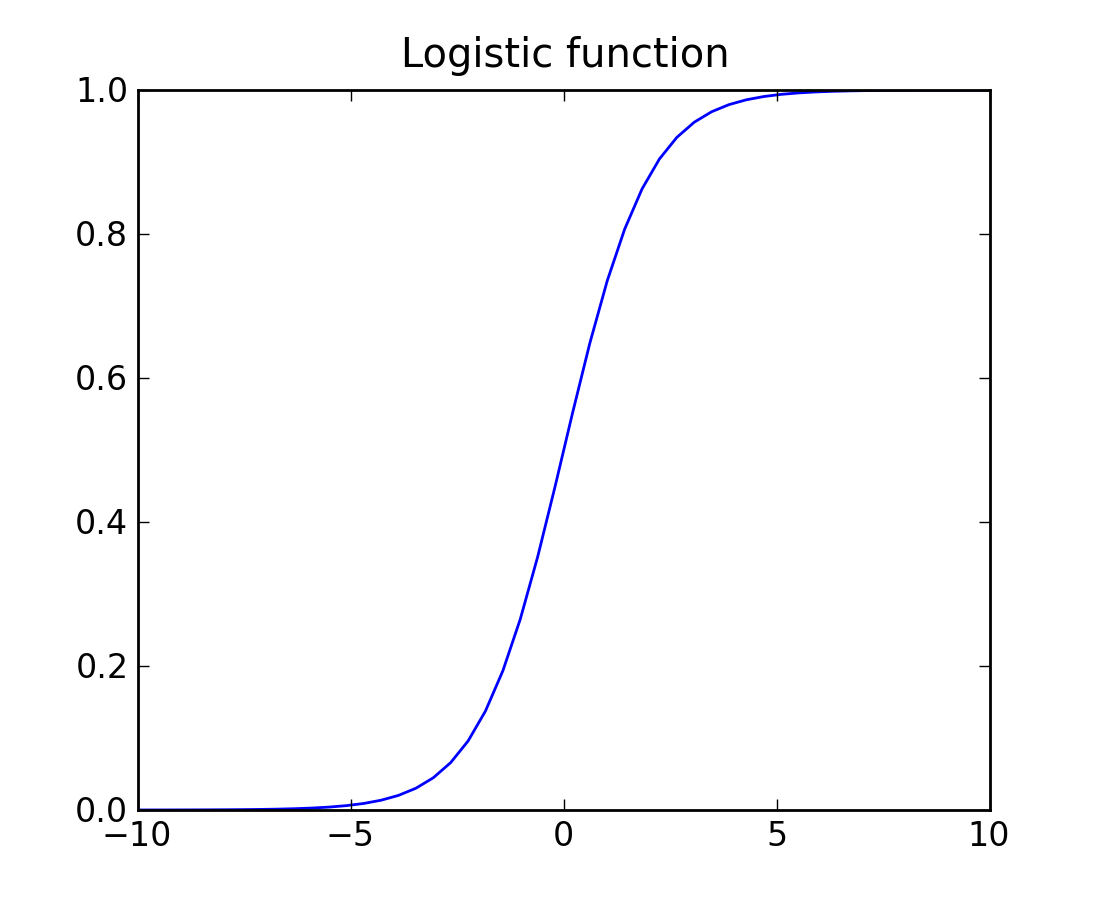
\includegraphics[scale=0.5]{pic/LR_EXAMPLE}
 \caption{Logistic Regression Example}
\end{figure}
\end{comment}

\begin{comment}
\textbf{An example of a cumulative distribution function plot of logistic
regression is shown below, which has a "S" shaped curves between 0 and 1.
shuai, in the figure, you said a=0, b=.5, what does this mean? }
\begin{figure}[h!]
   \centering
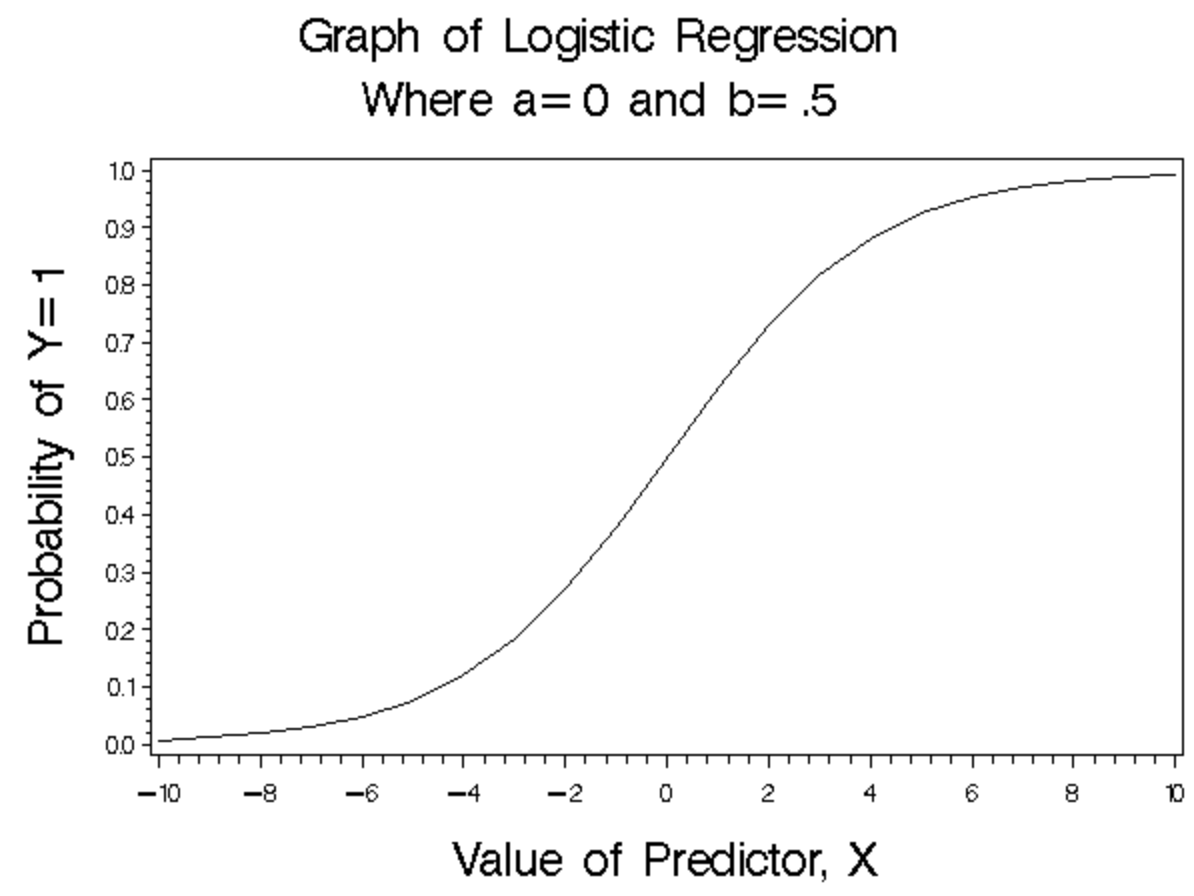
\includegraphics[width=0.4\textwidth]{LR.png}
 \caption{"S" shaped curve in logistic regression}
\end{figure}
\end{comment}

Parameters $\beta_0$ and $\beta_i$ are estimated by the maximum likelihood
estimation.
\begin{equation}
\ell(\beta_0,\ldots \beta_i) = \prod_{i:y_i=1} p(x_i)
\prod_{i^{'}:y_i{^{'}=0}} (1-p(x_{i^{'}}))
\end{equation}
For details on the derivation of the parameter estimations, please see
\citet{Hosmer2013}.

\subsection{A Logistic Regression Model}

The baseline model is a general linear logistic regression model.  Before the
model is presented, multicolinearity, or collinearity among variables is first
explored.

\subsubsection{Collinearity }

Multicollinearity or collinearity is a phenomenon in which two or more
predictor variables in a multiple regression model are highly correlated. In
this situation the coefficient estimates of the multiple regression may change
erratically in response to small changes in the model or the data.
\citep{belsley2005regression,Midi2010}.

A common method to detect collinearity is to examine the correlation matrix.
In the building of the logistic regression model, the following variables were
used GPA, ACT, HS.PERCENTILE, UNEMPLOYMENT.INDEX, PELL.GRANT, SCHOLARSHIP,
APP.COLLEGE, DISTANCE.BIN, HS.COUNTY.TIER, UNDERREPRESENTED, ETHNICITY.  The
correlation matrix  of the continuous variables is presented in Table
\ref{correlation_matrix}. % and scatter plot among these variables are shown in
Appendix B.  

%\paragraph{Logistic Regression Assumption}
%Logistic regression assumes \citet{lr_assumption1, Hosmer2013}: (1)
independence: observations are independent from each other; (2) linearity:
linear regression assumes that the outcome variable has a linear relationship
with the independent variables, or in the case of logistic regression, a linear
relationship between the logit of the independent variables and outcome
variables; (3) normal distribution is not necessary or assumed for the
dependent variable.


\begin{sidewaystable}[!htbp]
\small
\resizebox{\linewidth}{100pt}{
\begin{tabular}{@{\extracolsep{4pt}} lcccccccccc}
	
\\[-1ex]\hline 
\hline \\[-1.8ex] 
& GPA            & ACT    & \begin{tabular}[c]{@{}c@{}}HS.\\
PERCENTILE\end{tabular} & \begin{tabular}[c]{@{}c@{}}SCHOLAR-\\
SHIP\end{tabular} & \begin{tabular}[c]{@{}c@{}}PELL.\\ GRANT\end{tabular} &
\begin{tabular}[c]{@{}c@{}}TOTAL.\\ FREE.MONEY\end{tabular} &
\begin{tabular}[c]{@{}c@{}}OUT.OF.\\ POCKET\end{tabular} &
\begin{tabular}[c]{@{}c@{}}DISTANCE.\\ NUM\end{tabular} &
\begin{tabular}[c]{@{}c@{}}UNEMPLOYMENT.\\ INDEX\end{tabular} \\
                   \\ \hline
\hline \\[-1.8ex] 
                   
GPA         & 1       & 0.596  & \textbf{0.884}
& 0.612                 & -0.190
& 0.159             & -0.164
& -0.017            & -0.018 \\
ACT                & 0.596          & 1      & 0.469
& 0.586            & -0.275
& 0.069                    & -0.070
& -0.039             & 0.005\\
HS.PERCENTILE      & \textbf{0.884} & 0.469  & 1
& 0.594                                                   & -0.060
& 0.266                                                       & -.0271
& 0.011                                                   & -0.010\\
SCHOLARSHIP        & 0.612          & 0.586  & 0.594
& 1                                                       & 0.025
& 0.456                             & -0.456
& 0.031                                                   & 0.010\\
PELL.GRANT         & -0.190         & -0.275 & -0.060
& 0.025                                                   & 1
& \textbf{0.845}         & \textbf{-0.830}
& 0.023       & 0.132\\
TOTAL.FREE.MONEY   & 0.159          & 0.069  & 0.266
& 0.456           & \textbf{0.845}
& 1          & \textbf{-0.987}
& 0.037                                                   & 0.124\\
OUT.OF.POCKET      & -0.164         & -0.070 & -0.271
& -0.456         & \textbf{-0.830}
& \textbf{-0.987}                                             & 1
& -0.039                                                  & -0.045\\
DISTANCE.NUM       & -0.017         & -0.039 & 0.011
& 0.031        & 0.023
& 0.037            & -0.039
& 1                                                       & -0.010\\
UNEMPLOYMENT.INDEX & -0.018         & 0.005  & -0.010
& 0.010                                                   & 0.132
& 0.124          & -0.045
& -0.010         & 1 \\
\hline \\[-1.8ex]                                                            
\end{tabular}}
\caption{Pearson Correlation Matrix of all Numeric Variables} 
  \label{correlation_matrix} 
\end{sidewaystable}


As can be seen from Table, according to \citep{hinkle2003applied}, there exists
a very high correlation ( $0.9$ to $1$ or $-0.9$ to $-1$ ) between the monetary
variables such as between Out of Pocket and Total Free Money, and high
correlation( $0.7$ to $0.9$ or $-0.7$ to $-0.9$ ) between GPA and
HS.PERCENTILE, and between PELL Grant, Out of Pocket and Total Free Money.
Though this result is not surprising, and collinearity does not reduce the
predictive power or reliability of the model as a whole, collinearity it does
affect calculations regarding individual predictors and cause unstable
estimates of coefficients in regression analysis. That is, a multiple
regression model with correlated predictors can indicate how well the entire
bundle of predictors predicts the outcome variable, but it may not give valid
results about any individual predictor, or about which predictors are redundant
with respect to others.
 

\begin{comment}

\paragraph{Goodness of Fit for Logistic Regression Model}
%There are many tests that can be applied to evaluate the effectiveness of a
logistic regression model. Of them, four of the commonly used tests are (a)
tests of individual predictors, (b) overall model evaluation, (c) validation of
predicted probabilities, (d) goodness of fit statistics. \citet{lr_summary}

Goodness of fit statistics are the most used in the evaluation of logistic
regression model \citet{lr_summary} and several methods have been proposed.

The most straightforward method of evaluation  is to calculate the accuracy of
the fitted value.  A cut-of value (in percentage) , say 60\%, is chosen and any
predicted value greater than the cut-off will be a successful prediction and
any value below will be a failure. This analysis can be entered into a
two-by-two table, called a 'classification table' (or 'confusion matrix') as
shown below:
  
   % Please add the following required packages to your document preamble:
% \usepackage{multirow}
\begin{table}[h]
\centering
\label{my-label}
\begin{tabular}{|c|c|c|c|}
\hline
     & \multicolumn{3}{c|}{Actual Class}       \\ \hline
\multirow{3}{*}{\begin{tabular}[c]{@{}c@{}}Predicted\\  Class\end{tabular}} &
& Yes   & No    \\ \cline{2-4}
 & Yes & True Positive       & False Positive \\ \cline{2-4} 
& No  & \multicolumn{1}{l|}{False Negative} & True Negative  \\ \hline
\end{tabular}
\caption{Classification Table}
\end{table}

%The limitation of this measurement is that it does not have any measure of
significance.This means that 99\% accuracy can be excellent in some cases and
terrible in others. Another limitation is that it assumes equal cost for both
error types (false negatives and false positives).

Rather than a single cutoff value, another method of evaluation is  ROC
(Receiver Operating Characteristic curve)  which extends the cutoff to all
possible values from 0 to 1. An ROC curve (shown in the Figure
\ref{roc_example} below) illustrates the performance of a binary classifier
system as its discrimination threshold is varied.  The curve is created by
plotting the true positive rate against the false positive rate at various
threshold settings. Here, the dotted diagonal line is the random prediction. In
ROC curve, AUC (area under the curve) indicates the overall quality of the
model. In this case the AUC= 0.9342 which shows an excellent prediction. The
closer the ROC curve bulges towards the upper-left corner, the more accurate
the test is.

%The true-positive rate is also known as sensitivity or the sensitivity index
d', known as "d-prime" in signal detection and biomedical informatics, or
recall in machine learning. The false-positive rate is also known as the
fall-out and can be calculated as 1 - specificity. The ROC curve is thus the
sensitivity as a function of fall-out.

 
\begin{figure}[H]
   \centering
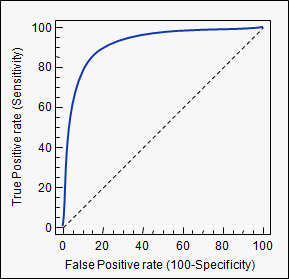
\includegraphics[width=2.5in, height=2in]{roc.png}
 \caption{an example of an ROC curve}
 \label{roc_example}
\end{figure}

\end{comment}



\subsubsection{Variable Selection}
In regression analysis with multiple variables, strategies have been designed
to select the best variables in the model. There are several approaches for
variable selection and stepwise regression is one of the most popular
semi-automated procedures \citep{Han2011}.


Stepwise variable selection include backward elimination, forward selection and
bidirectional elimination. A backward stepwise regression, for example, works
as follows: a) start with the model containing all potential predictors; b) try
subtracting one predictor at a time. Keeping the model if it improves the
measure of predictive accuracy; and c) iterate until no further improvement.

Several criterion have been proposed in variable selection to determine which
model works best. For logistic regression the most common criteria used in  are
BIC, AIC, AICc.  AIC (Akaike information criterion) is defined for a large
class of models fit by maximum likelihood and in logistic regression, AIC is
calculated as:
\begin{equation}
	AIC= -2 \times \ln(likelihood) + 2k
\end{equation}
where $k$ is the number of variables included in that model. For details,
please see  \citep{Han2011}. There is always a trade off between model
simplicity and how fit the model is. AIC is a measure to determine whether
extra variables are justified.
 	
In an enrollment model, say with 13 predictor variables, to get the optimal
model, a brute-force approach would have to evaluate $2^{13}$ possible models.
The stepwise variable selection evaluates only a limited number of models and
presents a heuristic solution to the problem in a fraction of time.

In our implementation, a backward stepwise procedure was adopted and the
detailed backward stepwise selection process is presented in Table \ref{back}.
In the table, the ``step" column represents the number of iterations; the
``model" column represents the model in each iteration; the ``AIC" column
represents the AIC value.  As can be seen, the process started with a full
model with all of the predictor variables and continued to seek models with
lower AIC.


Similar variable selection process was done using backwards selection, the
model end up only included variables: GPA , ACT, OUT.OF.POCKET,  APP.COLLEGE,
ETHNICITY, SCHOLARSHIP\_PER. 


%\begin{table}[]

%\begin{table}[]
\begin{sidewaystable*}
\centering
\caption{Backward stepwise model selection for enrollment model}
\label{back}
\begin{adjustbox}{width=1.05\textwidth}
\begin{tabular}{clll}
\hline
Step & Model                                                                   
& Variable Dropped                                        &
\multicolumn{1}{c}{AIC} \\ \hline
1    & \begin{tabular}[c]{@{}l@{}}MATRICULATION $\sim$ GPA + ACT +
HS.PERCENTILE + comb + APP.COLLEGE +,DISTANCE.NUM\\  + DISTANCE.BIN +
HS.COUNTY.TIER + HS.RAIDER.COUNTRY + GENDER + PELL.GRANT + \\ ETHNICITY +
UNDERREPRESENTED + UNEMPLOYMENT.INDEX +SCHOLARSHIP\_PER\end{tabular} &         
& 46262                   \\
2    & \begin{tabular}[c]{@{}l@{}}MATRICULATION $\sim$ GPA + ACT +
HS.PERCENTILE + APP.COLLEGE + DISTANCE.NUM \\ +DISTANCE.BIN + HS.COUNTY.TIER +
HS.RAIDER.COUNTRY + GENDER + PELL.GRANT + \\ ETHNICITY + UNDERREPRESENTED +
UNEMPLOYMENT.INDEX +SCHOLARSHIP\_PER\end{tabular}       & comb                 
& 46262                   \\
3    & \begin{tabular}[c]{@{}l@{}}MATRICULATION $\sim$ GPA + ACT +
HS.PERCENTILE + APP.COLLEGE + DISTANCE.NUM \\ +DISTANCE.BIN + HS.COUNTY.TIER +
HS.RAIDER.COUNTRY + GENDER + PELL.GRANT + \\ ETHNICITY + UNEMPLOYMENT.INDEX +
SCHOLARSHIP\_PER\end{tabular}                         & comb, UNDERREPRESENTED 
& 46260                   \\
4    & \begin{tabular}[c]{@{}l@{}}MATRICULATION $\sim$ GPA + ACT +
HS.PERCENTILE + APP.COLLEGE + DISTANCE.NUM + \\ DISTANCE.BIN + HS.COUNTY.TIER +
GENDER + PELL.GRANT + ETHNICITY \\ +UNEMPLOYMENT.INDEX +
SCHOLARSHIP\_PER\end{tabular}                                             &
comb, UNDERREPRESENTED, HS.RAIDER.COUNTRY               & 46258                
\\
5    & \begin{tabular}[c]{@{}l@{}}MATRICULATION $\sim$ GPA + ACT +
HS.PERCENTILE + APP.COLLEGE + DISTANCE.BIN + \\ HS.COUNTY.TIER + GENDER +
PELL.GRANT + ETHNICITY +\\  UNEMPLOYMENT.INDEX + SCHOLARSHIP\_PER\end{tabular} 
& comb, UNDERREPRESENTED, HS.RAIDER.COUNTRY, DISTANCE.NUM & 46257              
\\
\hline
\end{tabular}
\end{adjustbox}
\end{sidewaystable*}
%\end{table}

%\subsubsection{Residual Analysis}

\subsubsection{Training, Testing and Results for Enrollment Data}
The data from academic years from 2008-2009 to 2011-2012 is used as training
data  and the data from academic year 2012-2013 as testing data. The training
data has 30,083 entries and the testing data has 5,260 entries. The general
logistic regression model derived from the backward stepwise selection was used
as the baseline model.


The summary statistics of logistic regression model is shown in Table 
\ref{lr_summary}.  In the table, the odds ratio is usually reported in
logistics regression model to interpret categorical variables but not good for
nonlinear variables \citep{DesJardins2006, long2006regression}. 

%We plot the predicted probability against a subgroup to see the relationship
%of the independent variables and dependent variable.

Applicants with lower ACT are less likely to  enroll, however, applicants with
higher GPA are more likely to enroll. HS.PERCENTILE does not impact the
enrollment results very much. Foreign and unknown are less likely to enroll,
and two and more are the most likely  group to enroll. If applicant is
underrepresented, it's less likely to enroll. Distance Bins except Bin 1
(closest) are all less inclined to  enroll. College  of engineering is the
mostly to enroll among all the colleges. Scholarship (SCHOLARSHIP\_PER) have
impact on the enrollment -- the more scholarship that  one receive, the more
likely it will be enrolled. The unemployment index (0.9847), representing
economy, has little impact of on the enrollment.


\begin{table}[]
\centering
\begin{adjustbox}{width=1.05\textwidth}

\begin{tabular}{lcccllcc}
\\[-1.8ex]\hline
\hline

                               & Estimate & Std. Error & z value  &
Pr(\textgreater|z|) & Significant & 2.50\% & 97.50\% \\ 
 \hline
(Intercept)                     & 2.5934   & 0.1476     & 6.4600   & 0.0000    
& ***         & 1.9423 & 3.4639  \\
GPA                             & 1.3405   & 0.0463     & 6.3300   & 0.0000    
& ***         & 1.2242 & 1.468   \\
ACT                             & 0.9630   & 0.0038     & -9.8200  & 0.0000    
& ***         & 0.9558 & 0.9703  \\
HS.PERCENTILE                   & 0.9906   & 0.0011     & -8.8100  & 0.0000    
& ***         & 0.9885 & 0.9927  \\
APP.COLLEGEED                   & 0.9429   & 0.0493     & -1.1900  & 0.2331    
&             & 0.8561 & 1.0385  \\
APP.COLLEGEEG                   & 1.3506   & 0.0468     & 6.4200   & 0.0000    
& ***         & 1.2322 & 1.4806  \\
APP.COLLEGELA                   & 0.9670   & 0.0424     & -0.7900  & 0.4283    
&             & 0.8899 & 1.0508  \\
APP.COLLEGEN                    & 1.0696   & 0.0456     & 1.4800   & 0.1398    
&             & 0.9782 & 1.1696  \\
APP.COLLEGESM                   & 1.0530   & 0.0447     & 1.1600   & 0.2472    
&             & 0.9648 & 1.1494  \\
APP.COLLEGEUC                   & 0.9684   & 0.0419     & -0.7700  & 0.4441    
&             & 0.8921 & 1.0513  \\
DISTANCE.BIN02                  & 0.6498   & 0.0420     & -10.2600 & 0.0000    
& ***         & 0.5983 & 0.7054  \\
DISTANCE.BIN03                  & 0.4996   & 0.0737     & -9.4100  & 0.0000    
& ***         & 0.4323 & 0.5772  \\
DISTANCE.BIN04                  & 0.5819   & 0.0826     & -6.5600  & 0.0000    
& ***         & 0.4949 & 0.6841  \\
DISTANCE.BIN05                  & 0.4346   & 0.0843     & -9.8900  & 0.0000    
& ***         & 0.3683 & 0.5126  \\
DISTANCE.BIN06                  & 0.3029   & 0.1124     & -10.6200 & 0.0000    
& ***         & 0.243  & 0.3776  \\
HS.COUNTY.TIERTier2             & 0.8634   & 0.0495     & -2.9700  & 0.0030    
& **          & 0.7836 & 0.9514  \\
HS.COUNTY.TIERTier3             & 1.0881   & 0.0927     & 0.9100   & 0.3627    
&             & 0.9073 & 1.305   \\
HS.COUNTY.TIERTier4             & 0.6191   & 0.0803     & -5.9700  & 0.0000    
& ***         & 0.529  & 0.7247  \\
HS.COUNTY.TIERTier5             & 0.7649   & 0.1010     & -2.6500  & 0.0080    
& **          & 0.6274 & 0.9324  \\
HS.COUNTY.TIERTier6             & 0.8602   & 0.0791     & -1.9000  & 0.0570    
& .           & 0.7366 & 1.0046  \\
PELL.GRANT                      & 1.0002   & 0.0000     & 27.5700  & 0.0000    
& ***         & 1.0001 & 1.0002  \\
ETHNICITYBlackOrAfricanAmerican & 1.0272   & 0.0870     & 0.3100   & 0.7581    
&             & 0.8661 & 1.2182  \\
ETHNICITYForeign                & 1.4361   & 1.0153     & 0.3600   & 0.7215    
&             & 0.1679 & 12.2457 \\
ETHNICITYHawaiian               & 1.7012   & 0.3974     & 1.3400   & 0.1813    
&             & 0.7922 & 3.8216  \\
ETHNICITYHispanic               & 1.1814   & 0.1085     & 1.5400   & 0.1245    
&             & 0.955  & 1.4614  \\
ETHNICITYIndianAlaskan          & 1.3713   & 0.2534     & 1.2500   & 0.2128    
&             & 0.8348 & 2.261   \\
ETHNICITYTwoMore                & 1.7766   & 0.1061     & 5.4200   & 0.0000    
& ***         & 1.4435 & 2.1877  \\
ETHNICITYUnknown                & 0.4939   & 0.1265     & -5.5800  & 0.0000    
& ***         & 0.3848 & 0.632   \\
ETHNICITYWhite                  & 1.3417   & 0.0816     & 3.6000   & 0.0003    
& ***         & 1.1433 & 1.5746  \\
UNEMPLOYMENT.INDEX              & 0.9655   & 0.0059     & -5.9100  & 0.0000    
& ***         & 0.9544 & 0.9768  \\
SCHOLARSHIP\_PER                & 1.4894   & 0.0933     & 4.2700   & 0.0000    
& ***         & 1.2403 & 1.7883     \
\\
\\
AIC: 47044\\
Degrees of Freedom: 35330 \\
Null Deviance:      48952 \\
Residual Deviance: 46980

\\
\hline
\multicolumn{7}{l}{\scriptsize{$^{***} p=0.000$, $^{**} p<0.001$, $^*
p<0.01$,$^{.}p<0.05$}}
\end{tabular}
\end{adjustbox}
\caption{Summary statistics of logistic regression for enrollment model}
\label{lr_summary}
\end{table}


        

\begin{table}[]
\centering
\caption{Summary statistics of logistic regression for graduation model}
\label{lr_summary2}
\begin{adjustbox}{width=1.05\textwidth}
\begin{tabular}{llllllll}
\hline
\hline
Coefficients:                   & Estimate & Std. Error & z value &
Pr(\textgreater|z|) & Significant & 5\%    & 95\%   \\
(Intercept)                     & 2.6008   & 0.1576     & 3.1800  & 0.0015     
& **          & 1.2737 & 2.1390 \\
GPA                             & 2.6872   & 0.0505     & 7.9640  & 0.0000     
& ***         & 1.3757 & 1.6242 \\
ACT                             & 2.3540   & 0.0042     & -7.5840 & 0.0000     
& ***         & 0.9622 & 0.9755 \\
HS.PERCENTILE                   & 3.4288   & 0.0012     & -8.1700 & 0.0000     
& ***         & 0.9886 & 0.9924 \\
APP.COLLEGEED                   & 2.4349   & 0.0531     & -0.8630 & 0.3879     
&             & 0.8753 & 1.0423 \\
APP.COLLEGEEG                   & 2.6597   & 0.0506     & 4.4450  & 0.0000     
& ***         & 1.1523 & 1.3610 \\
APP.COLLEGELA                   & 2.6243   & 0.0458     & -1.2560 & 0.2090     
&             & 0.8757 & 1.0180 \\
APP.COLLEGEN                    & 2.4402   & 0.0492     & 1.0520  & 0.2929     
&             & 0.9712 & 1.1420 \\
APP.COLLEGESM                   & 1.8190   & 0.0483     & 0.9280  & 0.3532     
&             & 0.9660 & 1.1323 \\
APP.COLLEGEUC                   & 1.5408   & 0.0451     & -1.3450 & 0.1787     
&             & 0.8740 & 1.0136 \\
DISTANCE.BIN02                  & 1.6403   & 0.0446     & -8.8600 & \textless
2e-16     & ***         & 0.6256 & 0.7246 \\
DISTANCE.BIN03                  & 1.4453   & 0.0794     & -7.4110 & 0.0000     
& ***         & 0.4870 & 0.6325 \\
DISTANCE.BIN04                  & 1.2751   & 0.0889     & -5.3070 & 0.0000     
& ***         & 0.5391 & 0.7221 \\
DISTANCE.BIN05                  & 2.1893   & 0.0911     & -7.4790 & 0.0000     
& ***         & 0.4356 & 0.5877 \\
DISTANCE.BIN06                  & 2.4776   & 0.1223     & -8.0080 & 0.0000     
& ***         & 0.3073 & 0.4594 \\
HS.COUNTY.TIERTier2             & 1.6972   & 0.0534     & -3.9420 & 0.0001     
& ***         & 0.7418 & 0.8844 \\
HS.COUNTY.TIERTier3             & 1.8727   & 0.1002     & 0.2980  & 0.7657     
&             & 0.8738 & 1.2149 \\
HS.COUNTY.TIERTier4             & 2.0888   & 0.0873     & -5.9900 & 0.0000     
& ***         & 0.5135 & 0.6844 \\
HS.COUNTY.TIERTier5             & 2.7186   & 0.1101     & -3.4020 & 0.0007     
& ***         & 0.5736 & 0.8240 \\
HS.COUNTY.TIERTier6             & 2.3776   & 0.0859     & -3.0990 & 0.0019     
& **          & 0.6652 & 0.8826 \\
PELL.GRANT     & 1.1828   & 0.0000     & 22.9390 & 0.0000     & ***
& 1.0001 & 1.0002 \\
ETHNICITYBlackOrAfricanAmerican & 2.2082   & 0.0925     & 1.1540  & 0.2483     
&             & 0.9558 & 1.2958 \\
ETHNICITYForeign                & 2.5987   & 1.1780     & -0.6230 & 0.5331     
&             & 0.0432 & 2.8233 \\
ETHNICITYHawaiian               & 2.3044   & 0.4322     & 1.3140  & 0.1890     
&             & 0.8720 & 3.6575 \\
ETHNICITYHispanic               & 4.2355   & 0.1170     & 1.8430  & 0.0654     
& .           & 1.0234 & 1.5040 \\
ETHNICITYIndianAlaskan          & 1.4693   & 0.2690     & 1.1760  & 0.2396     
&             & 0.8799 & 2.1367 \\
ETHNICITYTwoMore                & 3.1371   & 0.1151     & 5.4470  & 0.0000     
& ***         & 1.5494 & 2.2628 \\
ETHNICITYUnknown                & 2.5971   & 0.1364     & -6.5000 & 0.0000     
& ***         & 0.3287 & 0.5149 \\
ETHNICITYWhite                  & 3.4567   & 0.0864     & 3.0690  & 0.0021     
& **          & 1.1312 & 1.5032 \\
UNEMPLOYMENT.INDEX              & 1.0000   & 0.0060     & -9.7690 & \textless
2e-16     & ***         & 0.9336 & 0.9522 \\
SCHOLARSHIP\_PER                & 1.0000   & 0.1010     & 5.1330  & 0.0000     
& ***         & 1.4221 & 1.9823    \\
\\
AIC: 4722\\
Degrees of Freedom: 3998 \\
Null Deviance:      5494.2 \\
Residual Deviance: 4684.1
\\
\hline
\multicolumn{7}{l}{\scriptsize{$^{***} p=0.000$, $^{**} p<0.001$, $^*
p<0.01$,$^{.}p<0.05$}}

\end{tabular}
\end{adjustbox}
\end{table}


Table \ref{lr_summary2} shows the summary statistics of graduation model. The
GPA and scholarship both significant impact on the graduation. The higher the
GPA and the higher the scholarship a student have, the more likely that the
student will be graduated. Two and more ethnicity has the highest likelihood to
graduate among all the ethnicities, while foreign students are the least
likely to graduate. Nursing school is the least likely to graduate from. 



The cut-off value for enrollment is set to 0.5. So if  $p(x) \geq 0.5$, then
enrollment;  otherwise, not enroll, then the accuracy and performance indicator
of the model is presented in Table  \ref{accuracy_model}.  
%\textbf{ Please explain this table }.

%\textbf{
%The accuracy of the logistic regression model is 61.9 while the AUC is 0.658,
%and the data is not biased towards positive or negative class as shown in
%\citep{Marsh2004}.} 

% Please add the following required packages to your document preamble:
% \usepackage{multirow}
\begin{table}[]
\centering
\begin{threeparttable}
\begin{tabular}{|l|c|c|l|l|l|}
\hline
\multicolumn{1}{|c|}{Model}          & \multicolumn{1}{l|}{AUC} & Accuracy
& Enrolled                                                          &
\begin{tabular}[c]{@{}l@{}}True Positive/\\ Negative Rate\end{tabular} &
\begin{tabular}[c]{@{}l@{}}False Positive/\\ Negative Rate\end{tabular} \\
\hline
\multirow{2}{*}{Logistic Regression} & \multirow{2}{*}{0.658}   &
\multirow{2}{*}{0.619 \tnote{*} } &
\multirow{2}{*}{\begin{tabular}[c]{@{}l@{}}Yes\\ No\end{tabular}}	 & 0.646 &
0.414                 \\
\cline{5-6} &  &   &  & 0.586            & 0.354
\\ \hline
\end{tabular}
\begin{tablenotes}\footnotesize
\item[*] 95\% CI
\end{tablenotes}
\end{threeparttable}
\caption{Accuracy of Enrollment Prediction from Logistic Regression Model }
\label{accuracy_model}
\end{table}

\begin{comment}
\begin{table}[!ht]
\centering
\begin{threeparttable}
\begin{tabular}{|l|c|c|l|l|l|}
\hline
\multicolumn{1}{|c|}{Model}          & \multicolumn{1}{l|}{AUC} & Accuracy
& Enrolled                                                          &
\begin{tabular}[c]{@{}l@{}}True Positive/\\ Negative Rate\end{tabular} &
\begin{tabular}[c]{@{}l@{}}False Positive/\\ Negative Rate\end{tabular} \\
\hline
\multirow{2}{*}{Logistic Regression} & \multirow{2}{*}{---}   &
\multirow{2}{*}{--- \tnote{*} } &
\multirow{2}{*}{\begin{tabular}[c]{@{}l@{}}Yes\\ No\end{tabular}}	 & -----
& ---                                                                      \\
\cline{5-6} &  &   &  & ----         & ---- \\ \hline
\end{tabular}
\begin{tablenotes}\footnotesize
\item[*] 95\% CI
\end{tablenotes}
\end{threeparttable}
\caption{Accuracy of Graduation Prediction from Logistic Regression Model }
\label{accuracy_model}
\end{table}
\end{comment}

\begin{comment}
\textbf{Rather than the use of 0.5 as the discrimination threshold,  a receiver
operating characteristic (ROC) curve is used by plotting the true positive rate
(TPR) against the false positive rate (FPR) at various threshold settings, }
let the discrimination threshhold be $\theta$, which ranges from 0 to 1,  the
ROC curve is presented in Fig \ref{log_ROC}:


\textbf{Here, for example, when $\theta = 0.5$, it shows that ....etc.   when
$\theta = 0.5$, it shows that ....etc. ...}

\textbf{what does the ROC curve tell you, other than accuracy? }

 \begin{figure}[!ht]
   \centering
 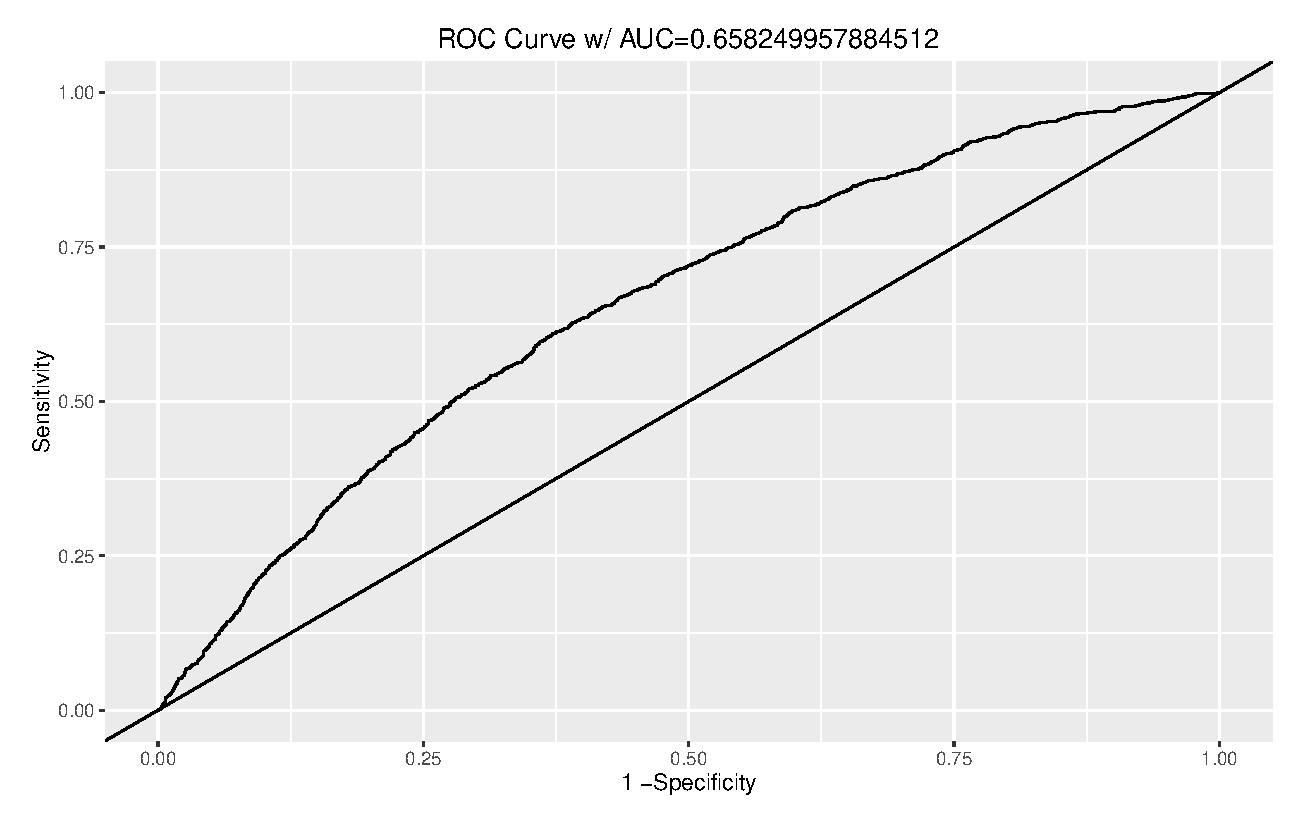
\includegraphics[scale=0.70]{pic/model_roc.eps}
 \caption{ROC Curve of the Logistic Model }
 \label{log_ROC}
\end{figure}

\end{comment}
  
  
  


\subsection{Logistic Regression Tree Model, Support Vectors Machines Models,
and Neural Network }
A logistic regression tree model extends the baseline logistic regression model
and uses a \textit{divide and conquer} strategy to divide  a complex set of
data into many subsets such that a linear logistic regression model adequately
fits the data in each subset. The division of the data into subset is performed
recursively, one variable at a time, and results in the partitions as a binary
decision tree \citep{harrell2013regression_book}.

The logistic tree with unbiased selection (LOTUS) algorithm \citep{lotus2}  is
selected in this research for the automation of a logistic regression tree.
LOTUS allows the nonlinear feature of the data sets to be modeled without
transforming the variables and compares favorable with standard stepwise
logistic regression \citep{lotus_app1,lotus_app2}. %The LOTUS implementation of
the logistic regression tree is used in this analysis; for details, please see
\citep{lotus2}.


\subsection{Results of Various Models on Enrollment and Graduation Predication}
\subsubsection{Results on Enrollment and Graduation Predication}

In this research, two logistic regression trees are being constructed: one for
enrollment, one for graduation.  In the construction of these tree models, the
variables used in these two tree models and their role in the tree models are
listed in the table below. Here, D represents the dependent variable, S is used
as a numerical variable to split the tree, C represents categorical variables
to split the tree, F represents the decision variables used in the logistic
regression function at the tree node.  The model accuracy for the logistic
regression trees are presented in the Tables \ref{accuracy_model_enroll}.
%\textbf{removed  HS.COUNTY.TIER} and \ref{accuracy_model_graduation}.

\begin{table}[h]
\centering
\begin{tabular}{|l|c|c|c|c|}
\hline
 %& \multicolumn{2}{c|}{Variables} & \multicolumn{2}{c|}{Variables} \\ \hline
\multicolumn{1}{|c|}{\multirow{2}{*}{Column}} & \multicolumn{2}{c|}{Enrollment}
& \multicolumn{2}{c|}{Graduation}                            \\ \cline{2-5}
\multicolumn{1}{|c|}{}                        & Name                          &
Type                     & Name                          & Type
\\ \hline
1                                             & Enrolled                      &
D                        & Enrolled                      & X
\\ \hline
2                                             & GPA                           &
S                        & GPA                           & S
\\ \hline
3      & Tier   & C    &   Tier   & C    \\ \hline
4    & Raider     & C   &   Raider  & C   \\ \hline
5   & ACT    & S  &  ACT    & S     \\ \hline
6   & Underrepresented & C     & Underrepresented    & C   \\ \hline
7    & Gender   & C   &  Gender  & C   \\ \hline
8   & Ethnicity    & C     & Ethnicity   & C      \\ \hline
9   & Scholarship(\$)    & F   & Scholarship(\$)     & F    \\ \hline
10  & Scholarship(\%)   & F     & Scholarship(\%)     & F  \\ \hline
11  & Estimated Tuition  & S    & Estimated Tuition  & S   \\ \hline
12  & Graduate   & X     &   Graduate        & D         \\ \hline
\end{tabular}
\caption{Variables Used in The Model}
\end{table}

% Please add the following required packages to your document preamble:
% \usepackage{multirow}
\begin{table}[!ht]
\centering
\begin{threeparttable}
\begin{tabular}{|l|c|c|l|l|l|}
\hline
\multicolumn{1}{|c|}{Model}          & \multicolumn{1}{l|}{AUC} & Accuracy
& Enrolled                                                          &
\begin{tabular}[c]{@{}l@{}}True Positive/\\ Negative Rate\end{tabular} &
\begin{tabular}[c]{@{}l@{}}False Positive/\\ Negative Rate\end{tabular} \\
\hline
\multirow{2}{*}{Logistic Regression Tree} & \multirow{2}{*}{0.618}   &
\multirow{2}{*}{0.62 \tnote{*} } &
\multirow{2}{*}{\begin{tabular}[c]{@{}l@{}}Yes\\ No\end{tabular}}	 & 0.65
& 0.414                                                                      \\
\cline{5-6} &  &   &  & 0.586          & 0.35 \\ \hline
\end{tabular}
\begin{tablenotes}\footnotesize
\item[*] 95\% CI
\end{tablenotes}
\end{threeparttable}
\caption{Accuracy of Enrollment Prediction from Logistic Regression Tree Model
}
\label{accuracy_model_enroll}
\end{table}

\subsubsection{Results on Graduation Predication}

\begin{comment}
	

% Please add the following required packages to your document preamble:
% \usepackage{multirow}
\begin{table}[!ht]
\centering
\begin{threeparttable}
\begin{tabular}{|l|c|c|l|l|l|}
\hline
\multicolumn{1}{|c|}{Model}          & \multicolumn{1}{l|}{AUC} & Accuracy
& Enrolled                                                          &
\begin{tabular}[c]{@{}l@{}}True Positive/\\ Negative Rate\end{tabular} &
\begin{tabular}[c]{@{}l@{}}False Positive/\\ Negative Rate\end{tabular} \\
\hline
\multirow{2}{*}{Logistic Regression Tree} & \multirow{2}{*}{---}   &
\multirow{2}{*}{--- \tnote{*} } &
\multirow{2}{*}{\begin{tabular}[c]{@{}l@{}}Yes\\ No\end{tabular}}	 & ----
& ----                                                                     \\
\cline{5-6} &  &   &  & ----            & ---- \\ \hline
\end{tabular}
\begin{tablenotes}\footnotesize
\item[*] 95\% CI
\end{tablenotes}
\end{threeparttable}
\caption{Accuracy of Graduation Prediction from Logistric Regression Tree Model
}
\label{accuracy_model_graduation}
\end{table}
\end{comment}

Preliminary experience with other logistic based models such as support vector
machines, neural network,  suggest similar accuracy results. The accuracy of
prediction from support vector machines and neural network results are shown in
the tables \ref{accuracy_model_enrollment_svm} %and
\ref{accuracy_model_graduation_svm}%,
%and the accuracy of prediction from neural network are shown in tables
\ref{accuracy_model_enrollment_nn} and
  %\ref{accuracy_model_graduation_nn}.

\begin{table}[!ht]
\centering
\begin{threeparttable}
\begin{tabular}{|l|c|c|l|l|l|}
\hline
\multicolumn{1}{|c|}{Model}          & \multicolumn{1}{l|}{AUC} & Accuracy
& Enrolled                                                          &
\begin{tabular}[c]{@{}l@{}}True Positive/\\ Negative Rate\end{tabular} &
\begin{tabular}[c]{@{}l@{}}False Positive/\\ Negative Rate\end{tabular} \\
\hline
\multirow{2}{*}{Support Vector Machine} & \multirow{2}{*}{0.612}   &
\multirow{2}{*}{0.608 \tnote{*} } &
\multirow{2}{*}{\begin{tabular}[c]{@{}l@{}}Yes\\ No\end{tabular}}	 & 0.531
& 0.306                                                                     \\
\cline{5-6} &  &   &  & 0.694            & 0.469 \\ \hline

\multirow{2}{*}{Neural Network} & \multirow{2}{*}{0.611}   &
\multirow{2}{*}{0.616 \tnote{*} } &
\multirow{2}{*}{\begin{tabular}[c]{@{}l@{}}Yes\\ No\end{tabular}}	 & 0.647
& 0.425                                                                     \\
\cline{5-6} &  &   &  & 0.575            & 0.353 \\ \hline

\end{tabular}
\begin{tablenotes}\footnotesize
\item[*] 95\% CI
\end{tablenotes}
\end{threeparttable}
\caption{Accuracy of Enrollment Prediction from Support Vector Machine Model
and Neural Network}
\label{accuracy_model_enrollment_svm}
\end{table}


\begin{comment}
\begin{table}[!ht]
\centering
\begin{threeparttable}
\begin{tabular}{|l|c|c|l|l|l|}
\hline
\multicolumn{1}{|c|}{Model}          & \multicolumn{1}{l|}{AUC} & Accuracy
& Enrolled                                                          &
\begin{tabular}[c]{@{}l@{}}True Positive/\\ Negative Rate\end{tabular} &
\begin{tabular}[c]{@{}l@{}}False Positive/\\ Negative Rate\end{tabular} \\
\hline
\multirow{2}{*}{Support Vector Machine} & \multirow{2}{*}{---}   &
\multirow{2}{*}{--- \tnote{*} } &
\multirow{2}{*}{\begin{tabular}[c]{@{}l@{}}Yes\\ No\end{tabular}}	 & ----
& ----                                                                     \\
\cline{5-6} &  &   &  & ----            & ---- \\ \hline
\end{tabular}
\begin{tablenotes}\footnotesize
\item[*] 95\% CI
\end{tablenotes}
\end{threeparttable}
\caption{Accuracy of Graduation Prediction from Support Vector MachineModel }
\label{accuracy_model_graduation_svm}
\end{table}
\end{comment}

%\begin{comment}
The prediction of graduate prediction was done in the similar fashion. The
comparison metrics of the graduation model are shown in Table
\ref{grad_accuracy_table}:

\begin{table}[!ht]
\centering
\begin{threeparttable}
\begin{tabular}{|l|c|c|l|l|l|}
\hline
\multicolumn{1}{|c|}{Model}    & \multicolumn{1}{l|}{AUC} & Accuracy
& Graduated                                                          &
\begin{tabular}[c]{@{}l@{}}True Positive/\\ Negative Rate\end{tabular} &
\begin{tabular}[c]{@{}l@{}}False Positive/\\ Negative Rate\end{tabular} \\
\hline
\multirow{2}{*}{Logistic Regression} & \multirow{2}{*}{0.79}   &
\multirow{2}{*}{0.74 \tnote{*} } &
\multirow{2}{*}{\begin{tabular}[c]{@{}l@{}}Yes\\ No\end{tabular}}	 & 0.8
& 0.41                                                                     \\
\cline{5-6} &  &   &  & 0.59            & 0.2 \\ \hline

\multirow{2}{*}{Logistic Regression Tree} & \multirow{2}{*}{0.76}   &
\multirow{2}{*}{0.739 \tnote{*} } &
\multirow{2}{*}{\begin{tabular}[c]{@{}l@{}}Yes\\ No\end{tabular}}	 & 0.88
& 0.57                                                                    \\
\cline{5-6} &  &   &  & 0.43            & 0.12 \\ \hline

\end{tabular}
\begin{tablenotes}\footnotesize
\item[*] 95\% CI
\end{tablenotes}
\end{threeparttable}
\caption{Accuracy of Graduation Prediction from Logistic Regression and
Logistic Regression Tree}
\label{grad_accuracy_table}
\end{table}

Due to space limitations, Details of these advance models such as support
vector machine and neural network are not represented in the proposal. To
further develop these models to increase the prediction accuracy is the focus
of the rest of the study.

\section{Model Results}

The predictions of enrollment probabilities for six applications with different
levels of scholarship awards are listed in table \ref{prediction_sample}. Here,
the concatenate string under ``student'' represents the characteristic of the
student. For example, student ``2.9-Tier1-19-White'' represents an application
from a student with a high school GPA of 2.9,ACT score of 19, lives in Tier 1
region, and is of white ethnicity.   the number represents the probabilities of
enrollment in percentage of the corresponding scholarship awards, which spans
from 0 to 10,000.

\begin{table}[ht]
\centering
 \small
 \setlength\tabcolsep{4pt}
    \begin{tabular}{|c|c|c|c|c|c|c|c|c|c|c|c|}
    \hline
    \multicolumn{12}{ |c| }{GPA 2.9, ACT 19 }  \\ \hline
& Student               & 0       & 1000    & 2000    & 3000    & 4000    &
5000    & 6000    & 7000    & 8000    & 10000   \\ \hline
1& 2.9-Tier1-19-White    & 59.55 & 64.63 & 69.39 & 73.77 & 77.73 & 81.24 &
84.31 & 86.96 & 89.22 & 91.72 \\ \hline
2& 2.9-Tier5-19-White    & 36.96 & 40.20 & 43.53 & 46.92 & 50.34 & 53.75 &
57.13 & 60.45 & 63.67 & 69.74 \\ \hline
     \multicolumn{12}{ |c| }{GPA 3.3, ACT  25 }   \\ \hline
3& 3.3-Tier1-25-Hispanic & 23.80 & 27.44 & 31.42 & 35.69 & 40.20 & 44.88 &
49.65 & 54.43 & 59.13 & 67.97 \\ \hline
4& 3.3-Tier1-25-White    & 55.60 & 59.32 & 62.94 & 66.42 & 69.72 & 72.84 &
75.75 & 78.43 & 80.90 & 85.17 \\ \hline
    \multicolumn{12}{ |c| }{GPA 3.8,ACT 28 }     \\ \hline
5& 3.8-Tier1-28-White    & 42.29 & 46.05 & 49.85 & 53.65 & 57.41 & 61.08 &
64.63 & 68.03 & 71.25 & 77.07 \\ \hline
6& 3.8-Tier4-28-White    & 20.54 & 22.87 & 25.37 & 28.05 & 30.89 & 33.89 &
37.02 & 40.26 & 43.60 & 50.41 \\ \hline
    \end{tabular}
\caption{ Prediction Of Enrollment Under Different Levels of  Scholarships}
\label{prediction_sample}
\end{table}

Several interesting observations can be seen from these predictions, a) as GPA
increases, the probability of enrollment decreases; b) local students (Tier 1)
have a larger probability of enrollment than distance students (other tiers);
c) as financial aid increases, the probability of enrollment increases; yet
increase in probability with respect to scholarship is different among
different student groups.

Comparison of students 1 an 2, though both students have the same GPA and ACT
score and are of the same ethnicity, student 1 who lives in tier 1 has a much
higher probability of enrollment than that of student 2 who live in tier 5.

Comparison of students 1 an 5, though both students lives in the same region,
tier 1, are of the same ethnicity, student 1, who has a GPA of 2.9, ACT of 19,
has a higher probability of enrollment than student 5, who has a GPA of 3.8 and
ACT of 28.

Comparison of students 3 and 4, though both students lives in the same region,
tier 1, have the same GAP of 3.3 and ACT of 25, student 1, who is of White
ethnicity, has a higher probability of enrollment than student 5, who is of
Hispanic ethnicity.

In all these cases, the probability of enrollment increases with the increase
of scholarship awards. Though these observations are not surprising, accurate
quantitative prediction of these probabilities are essential to the allocation
of scholarship.

However, it has to mention that the prediction of these probabilities alone has
not yet solve the fundamental problems for the enrollment management team of
any higher institution;  The optimal allocation of the scholarship to optimize
an institution's revenue, and the formation of concrete policies and action
plans needs to be solved. This is the second part of the research and is
addressed in the following sections.



\begin{comment}
Figure \ref{dt_plot_example} is an example of a decision tree. 

\begin{figure}[h!]
   \centering
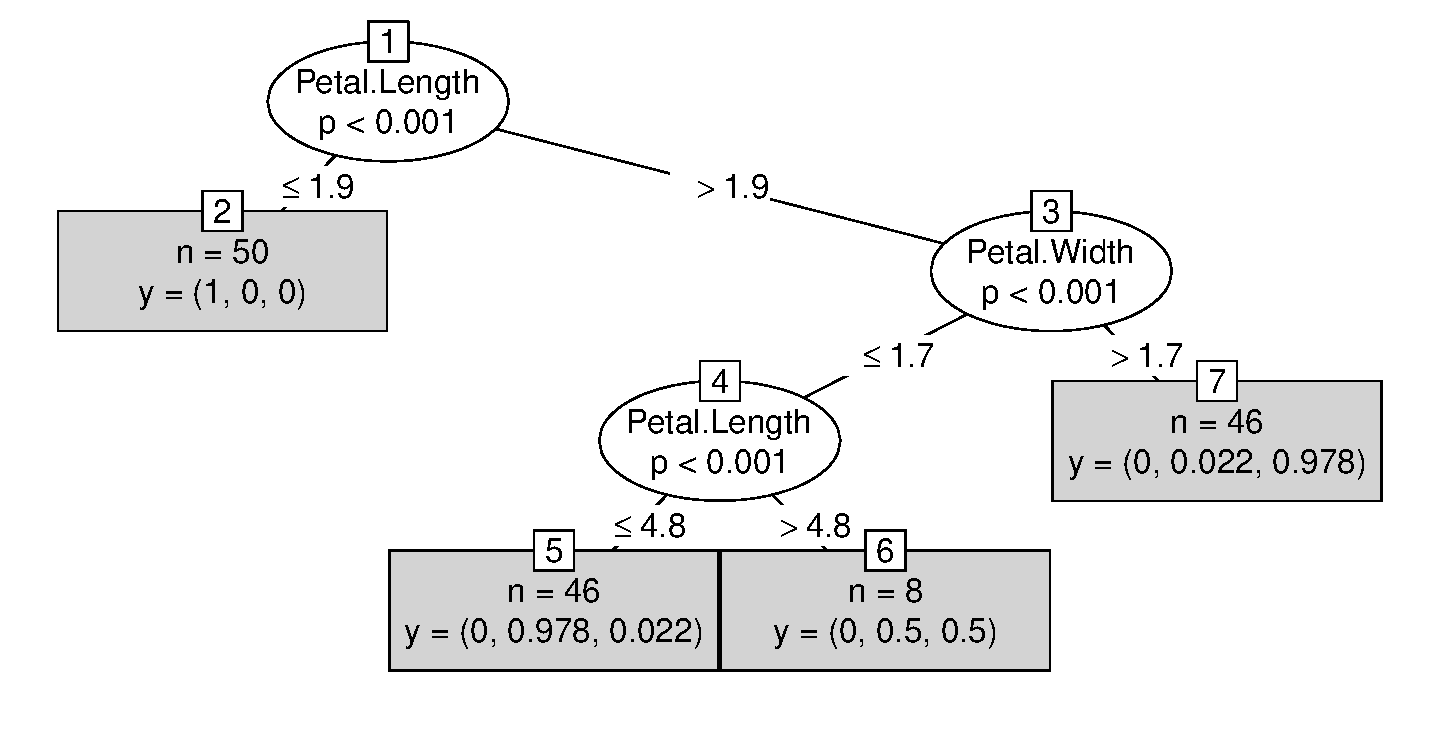
\includegraphics[width=0.8\textwidth]{dt_example.eps}
 \caption{an example of decision tree}
 \label{dt_plot_example}
\end{figure}
\end{comment}

\chapter {Prediction Models on the Number of Years of Studies}
Enrollment management practitioners, however, should keep in mind that how
financial aid influences student retention is more complex than how it affects
student enrollment decisions.

In this chapter, we try to answer one question: how long will a student stay
before dropout. 
% what are the chacter of student who dropout.

\section{Introduction of retention and number of years of studies}
After enrollment, university switches focus on creating a great environment to
help intellectual development, preventing students from dropping out or
transferring out.  By doing so, the university can make intervention program to
give students more guidance in order to  improve enrollment quality. Higher
graduation rate is also important to get funding from government, maintaining
financial stability and improve reputation. The cost of higher education keeps
increasing but the funding from federal and state is decreasing, so it is
crucial for university to keep the dropout rate low.

From financial aid prospective, it is ideal to give more aid to those who are
less likely to dropout. From students' perspective, staying in school and
eventually getting a degree is important to get a better career which leads to
better financial status \citep{thomas2002}. 


Studies found that first-year students are the most vulnerable to dropout.
Freshmen face drastic changes not only in academic challenge but also all kinds
of social challenge. Therefore first-year students retention are mostly studied
\citep{Permzadian2016,Kovacic10earlyprediction,Horstmanshof2007,Noble2007}. 


From early studies, dropout is affected by the interaction of students'
pre-enrollment characteristic (academic performance, finance, ethnicity, etc.) 
and academic experience (peer group interactions, interaction with faculty,
etc.). The higher degree of academic and social involvement and integration,
the more likely that students to complete the degree \citep{Tinto1975,
Tinto1982, Terenzini1981}. University is interested in identifying what factors
have an influence on the retention, and by doing analysis it can identify the
early stage hazard so as to improve the retention rate.

Typically, retention studies are interested in predicting whether a student
will dropout (1) or not (0). Studies focus on examining factors which influence
students' dropout or transfer. 
Classification prediction methods such as logistic regression, decision tree,
random forest were mostly
used\citep{dekker2009,AdamGaither2005,quadri2010drop,yu2010data,Herzog2006}.
Neural networks and boosting techniques yield better accuracy than the above
common classification methods \citep{Lin2009,zhang2010using,Herzog2006}.

Longitudinal study such as survival analysis is rarely studied in the retention
area, due to complex nature of the path to graduation \citep{Murtaugh1999,
Ishitani2003, zwick2005}. Survival analysis is a technique that estimate time
to the event of interest. For example, the event of interest for the retention
study is a student dropout or not and time is when does it happen.


Survival analysis can handle censored data, which participant's survival or not
cannot be represented at the point of interest :students are not observed or
not available because data collection ends while they are still in college.
Survival regression (Cox proportional hazards regression analysis) is able to
assign the probability to every period before or on the event of interest.
Those are some advantages that over regular classification methods in the
retention study. \citet{Ameri2016} compared Cox regression, SVM regression and
adboost to predict the when will a student dropout during early stage. The
cutoff semester was set to 6 (two years), which only consider the students who
are most likely not graduate.

The dropout rate at the university under study is about 60\%. As a result, it
is urgent and necessary to study the factors affected the dropout.  Development
of a predictive model could help to track students with potential transfer or
dropout and provide guidance in teaching, mentoring, financial aid, etc,.  



\section{Data Collection and Variables}

\subsection{Data Collection}

In this study, data included 6428 incoming freshmen students during 2006, 2007
and 2008 academic years. The latest data obtained is 2012 Fall, so the earliest
enrolled students from 2006 already stayed for seven academic years. The cutoff
value for the study is 5: any number of years greater than 5 are treated as 5.
The training data sets are 2006 and 2007, while the testing set is 2008.
Among them, 26\% freshmen stayed less than two years. 43\% were male, 57\% were
female. Ethnicity breakdown is as follows: 73.9\% Caucasian, African American
17.8\%, 2.2 \% Two and More, 2.1\% Asian, 2\% Hispanic, two \% Others. Table 
\ref{years_composite} shows the relation between average composite score and
number of years of stay.


\begin{figure}[ht]
   \centering
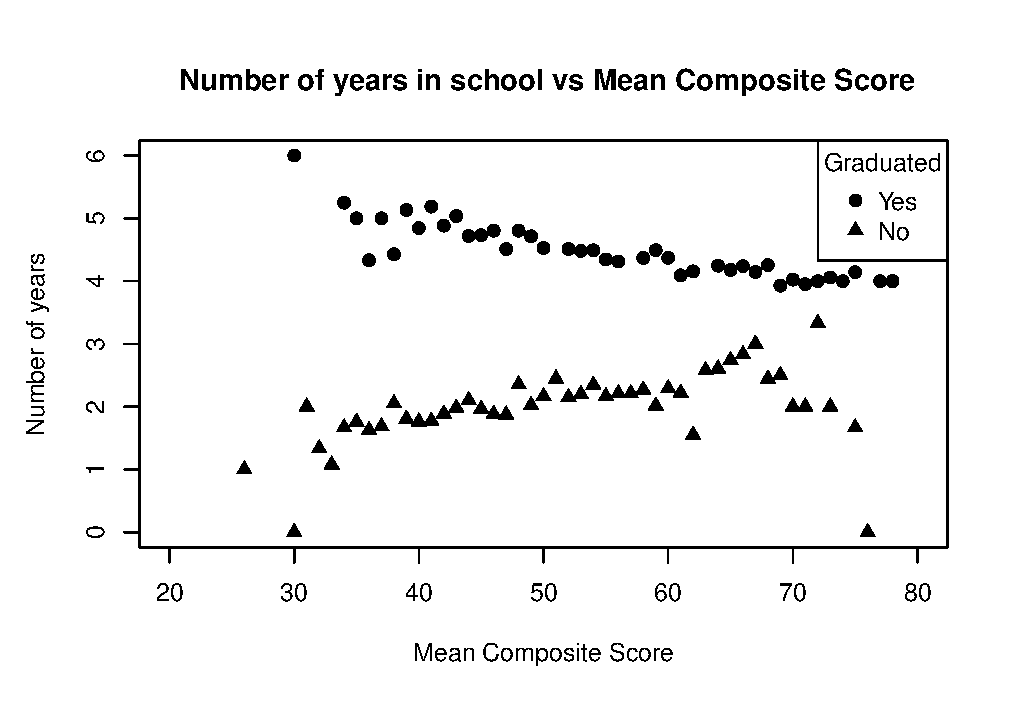
\includegraphics[width=5in,
height=3.5in]{pic/years_in_school_vs_composite_score.eps}
 \caption{Average Years in School vs Composite Score}
 \label{years_composite}
\end{figure}

Before 2013 Fall, the university used quarter system (4 quarters total for an
academic year) and converted to semester system(3 semesters for an academic
year) later. The number of years staying school is calculated as: $round(Last
Registered Term - First Term,0.5)$ for the convenience. For example, a student
enrolled in Fall 2006 and left in Spring 2010, the number of years stay is 3.5.



\subsection{Variables}
The predictions models for enrollment and graduation provided many factors
analysis for retention and time to degree study. Besides the previously
mentioned variables like demographics, pre-collegiate academic performance, and
financial background, variables such as campus experience (on or off campus
living, average class size, etc.), college academic performance (credit hours
taken, grades, etc.), and ongoing financial need.

Health and psychosocial variables were studied in the retention prediction.
Variables such as smoking, drinking, health-related quality of life, social
support, were found significantly related to the academic achievement and
retention \citep{deberard2004predictors, maney1990predicting,
musgrave1997personality, cutrona1994perceived}.

Variables selection for the number of years prediction followed by the
enrollment and graduation prediction. Unlike the studies \citep{Lin2009,
deberard2004predictors, dekker2009}, which tracked the after enrollment data
such as semester GPA and social activities, this research only used
pre-collegiate due to data collection limit.

The training data of the this study is from year 2006-2007 and 2007-2008, when
3999 students were enrolled. The testing data is from year 2008-2009, when 2355
students were enrolled. Since the data collection ends at 2012-2013, the latest

year of stay for testing data is 4.5 years. There are two types of students
here: students leave the college with or without getting a degree. Students who
graduate with a degree and without spend average 4.1 and 2.05 years
respectively.

The dependent variable for how long will stay has the following levels: 0, 0.5,
1, 1.5, 2, 2.5, 3, 3.5, 4, 4.5, 5. Students who stayed more than five years are
removed from the analysis due to the rarity. Although the dependent is
discreet, the problem is still a regression problem instead of a
classification problem because of dependent variable has a natural order.

\section{Methods and results}
\subsection{Prediction Models}

We can not apply survival analysis like \citep{Ameri2016} proposed,
because we have to consider those who stay more than 2 years. The event
of interest they used is the dropout and the cutoff year is 2 years,
which means the longest prediction of years of stay is 2 years. If we use
the similar setup, it is no going to help the objective where need the
prediction of number of years of stay not matter the student dropout or
not. If we set up the point of interest of event to 4, we will have
student graduated already and they are survival status are unknown before
the event of interest.

To answer the question how long will a student dropout, we compared
linear regression, support vector machine regression, random forest, CART,
stochastic gradient boosting to conduct the research. 

\textbf{Generalized Linear Model (GLM)} is a generalization of linear
regression which dependent variable has normal distribution and Gaussian error.
GLM broadens the the distribution to other family such like exponential and
binomial.  GLM is able to handle analyze the simultaneous interactions of
variables, including mixtures of categorical and continuous variables.

\textbf{ Support Vector Machines (SVMs)} are supervised classifiers used for
classification, regression and outlier detection. Given labeled data, the
algorithm outputs an optimal hyperplane or set of hyperplane, which separate
the data into different classes or for regression purpose.

%In a nutshell, the linear SVM is to optimize the 
In a simple two dimensions where the classes are linear separable. We have
labeled example $(x_1,y_1)$,...,$(x_n, y_n)$ with label $y_i = 1$ for inputs
$x_i$ in class 0 and $y_i = -1$ for inputs $x_i$ in class 1. The classification
boundary or hyperplane is defined as $w^T x +b = 0$, where w is the weight
vector and $b$ is the bias. The hyperplane can be represent by
different scale of $(w,b)$. The optimal one is defined as
$|w^T x +b | = 1$, where x is the data points closest to the hyperplane, for
instance the negative classification boundary is $w^T x +b = -1$ and positive
classification boundary is $w^T x +b  = 1$. As a results, the distance between
data point $x$ and the hyperplane $(w,b)$ is $ \frac{|w^T+b|}{||w||}=
\frac{1}{||w||}$, so the total distance to positive and to negative class,
defined as the margin $M$ is $\frac{2}{||w||}$.  The goal is to maximize margin
$M$ the separate the data points having 1 from those having 1, so we have to
minimize the $w^T$. The final problem of linear SVM is to optimize:

\begin{equation}
\text{minimize} \ \frac{2}{||w||^2},
\text{ subject to }
y_{i}(w^T x +b) \geq 1 \ \forall i
\end{equation}
where $y_i$ is either positive class (1) or negative class (-1).

\textbf{Support Vector Machine Regression (SVMR)} is a sub-category of SVM to
solve regression problem. 
SVM regression performs linear regression in the high-dimension feature space
using  $\epsilon$-insensitive loss and to reduce model complexity by
minimizing $||w||^2$. By introducing slack variables $\xi$, the model are able
to measure the error of training data outside the $\epsilon$-insensitive zone.
Thus, the SVM regression means solving the following minimization problem: 

\begin{equation}
    \begin{aligned}
     &   \text{minimize}
     & & \frac{1}{2} {||w||^2} + C \sum_{n=1}^{n}(\xi_i + \xi_i^+) \\
     & \text{subject to} 
     & & y_{i} - f(w,x_i) \leq  \epsilon + \xi^+, \\
     &&& f(w,x_i) - y_{i} \leq \epsilon + \xi, \\
     &&& \xi^i, \xi^+ \geq 0, i=1,\dots,n
    \end{aligned}
\end{equation}

where the $x_i$ is the training data and $y_i$ is target variable.


\textbf{Decision Trees} are commonly used to build classification and
regression model in a form of tree-like or shape. Decision tree methods
separate data into groups to grow branches. A decision tree contains root
nodes,
terminal nodes and internal nodes. Root node is the one on the topmost, usually
represent by the best attributes. Leaf nodes contain the final decision value
of the dependent variable. Internal nodes represent the value of attributes.
Algorithm used to build decision tree including ID3, C4.5, C5.0, CHAID, CRUISE,
etc. To split the tree, measurement algorithm like gini index, information gain
are used. For regression specifically, minimizing  residual sum of squares
(SSE):

\begin{equation}
	SSE = \sum_{i \in S_1} (y_i - \overline{y_1}) + \sum_{i \in S_2} (y_i -
	\overline{y_2})
\end{equation}

are used to split the value of an attribute. $\overline{y_1}$ and
$\overline{y_2}$ are the average values of the dependent variables in group
$S_1$ and $S_2$. 

%\textbf{Random forest} is 

\textbf{Stochastic gradient boosting} is a sub-category of boosting methods,
which convert weak learner to strong learner. A boosting model start building
the model using base machine learning algorithms with different distribution,
then the second model is generated based by correcting errors from the first
model. Decision tree with a fixed sized is typically used as the weak learner
in the gradient boosting.
The process stops until the limit of the base algorithm is reached or
certain accuracy is achieved. The estimate of response variables are 
consecutively becoming more accurate during the iterations.Stochastic gradient
boosting for regression problem uses square error as loss function. At each
iteration, a sample data was randomly selected from the full training data
without replacement. The weaker learner then is built on the sample data
instead of the full training data \citep{FRIEDMAN2002367}. 



    
We run two sets of experiments to evaluate the model performance. The first
experiment is 10-fold cross validation. Data used in this experiment is from
year 2006-2007 and 2007-2008. 
80\% of data were randomly chosen to build the model and 20\% percent of the
data were used to validate the model in each fold.
The final evaluation model is from the average metric of all the folds.
The second experiment is using data from 2008-2009 to predict the unseen
students.
    
\subsection{Model Metrics and Experiment Results}
Several metrics were used to evaluate the regression model:

The Root Mean Square Error (RMSE) is the most common goodness-of-fit measure.
This is the square root of the average square of the difference between our
prediction and actual values. RMSE is in the same units as predicted value.
\begin{equation}
\textbf{RMSE:}  \sqrt{\frac{1}{n}\sum_{n=1}^n (y_i-\hat{y}_i)^2}
\end{equation}

The mean absolute error (MAE) is used to measure the difference of forecasts to
the real outcomes.
\begin{equation}
\textbf{MAE} = \frac{1}{n}\sum_{i=1}^n \left| y_i - \hat{y_i}\right| 
\end{equation}



%We implemented all the methods in R programming language .
For SVM regression, we used linear kernel in R (implemented in e1071 package
\citep{e1071} using default settings). For GLM, we used regular regression
function in R base package. For decision tree, we used rpart package
\citep{rpart} in R. For stochastic gradient boosting. We implemented using
gbm package in R \citep{gbm}.
 
The results of the prediction models are as shown below:

\begin{table}[h]
\centering
\caption{Model Performance}
\label{num_year}
\begin{tabular}{|c|c|c|c|c|}
\hline
                             & \multicolumn{2}{c|}{10-Fold Cross Validation} &
\multicolumn{2}{c|}{Test Data} \\ \hline
Model                        & RMSE                  & MAE                   &
RMSE           & MAE           \\ \hline
GLM                          & 1.40                  & 1.2                   &
1.53           & 1.26          \\ \hline
SVM(Linear Kernel)           & 1.44                  & 1.20                  &
1.62           & 1.32          \\ \hline
%Random Forest                & 1.41                  & 1.21                 &
%1.41           & 1.24          \\ \hline
Decision Tree                         & 1.43                  & 1.24        &
1.43           & 1.23          \\ \hline
Stochastic Gradient Boosting & 1.40                  & 1.19                  &
1.40           & 1.19           \\ \hline
\end{tabular}
\end{table}


The results show that the tree based methods: decision trees and stochastic
gradient boosting yield lower RMS and MAE. Both algorithms are represented in
the form of tree structure. From table \ref{relatice_influ}, variables such as
GPA, HS.PERCENTILLE contribute the most to the model.

\begin{table}[h!]
\centering
\caption{Relative influence of variables in gradient boosting model}
\label{relatice_influ}
\begin{tabular}{|c|c|}
\hline
Variable                        & Relative Influence \\ \hline
GPA                             & 47.91771887        \\ \hline
HS.PERCENTILE                   & 12.9595027         \\ \hline
ACT                             & 7.050451247        \\ \hline
ETHNICITYTwoMore                & 6.706346519        \\ \hline
PELL.GRANT                      & 4.743360342        \\ \hline
SCHOLARSHIP\_PER                & 4.033307548        \\ \hline
UNEMPLOYMENT.INDEX              & 3.202687597        \\ \hline
ETHNICITYUnknown                & 2.83996864         \\ \hline
OUT.OF.POCKET                   & 1.770385883        \\ \hline
ETHNICITYHispanic               & 1.68325614         \\ \hline
DISTANCE.BIN04                  & 1.251210899        \\ \hline
COLLEGEN                    & 1.235771755        \\ \hline
DISTANCE.BIN05                  & 0.893538412        \\ \hline
DISTANCE.BIN02                  & 0.79644945         \\ \hline
DISTANCE.BIN03                  & 0.788177176        \\ \hline
COLLEGEEG                   & 0.783195486        \\ \hline
ETHNICITYWhite                  & 0.542182288        \\ \hline
COLLEGELA                   & 0.507483376        \\ \hline
COLLEGESM                   & 0.295005675        \\ \hline
COLLEGEED                   & 0                  \\ \hline
COLLEGEUC                   & 0                  \\ \hline
DISTANCE.BIN06                  & 0                  \\ \hline
ETHNICITYBlackOrAfricanAmerican & 0                  \\ \hline
ETHNICITYForeign                & 0                  \\ \hline
ETHNICITYHawaiian               & 0                  \\ \hline
ETHNICITYIndianAlaskan          & 0                  \\ \hline
\end{tabular}
\end{table}

\begin{figure}[ht]
   \centering
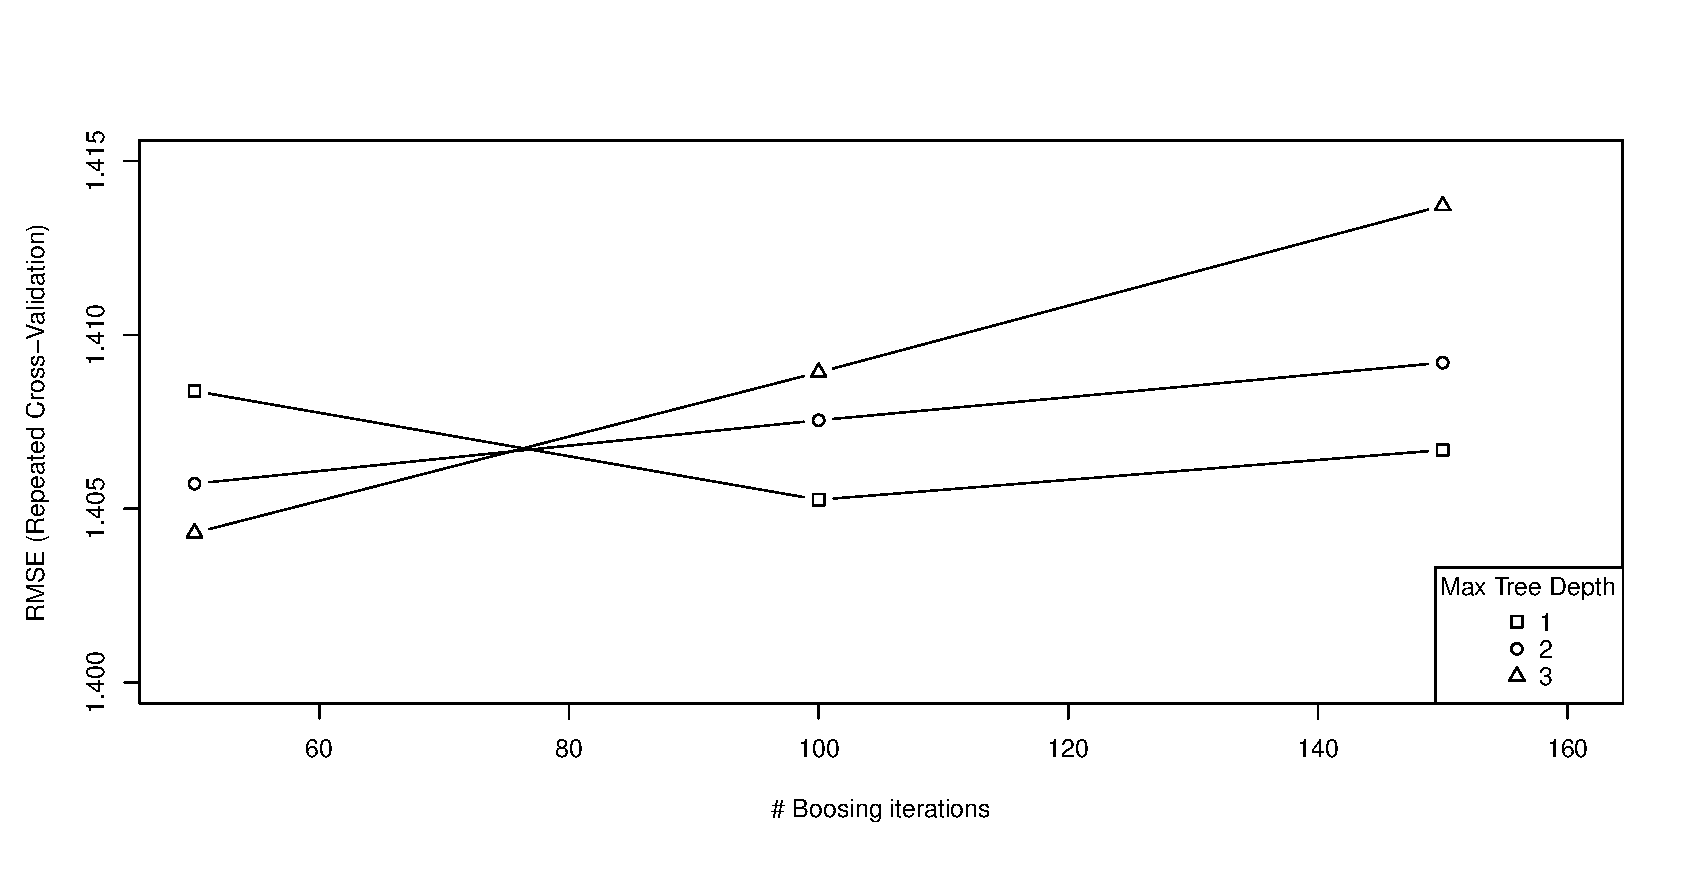
\includegraphics[width=5in,
height=3.5in,scale=0.5]{pic/Stochastic_boositing.eps}
 \caption{Stochastic booting procedure}
 \label{boosting}
\end{figure}



\chapter{Mathematical Models for Optimal Financial Aid  Allocation Problem }

The study of response to scholarship, though provided much insights to the
behavior of the students in responding to scholarship, has not addressed
fundamentally the allocation of limited financial aid to students.

For example, it is easy to see that local students requires less money while
students in far-away regions may require more money, it is still puzzling as a)
should we allocate the money to local students as they are our peanut and
butter students and requires less money or b) should we allocate the money to
far-away students as local students will come anyway? The solution to these
problems requires the solution of an optimization problem to optimally allocate
the financial aid.  This is the second part of the overall approach and is
addressed in this chapter.



\section{The Financial Aid Optimization Model}

\noindent Given a set of applicants and their probabilities of enrollment and
of graduation with respect to different levels of financial aids, the
optimization problem to be solved is to determine the financial aid to each
applicant so as to to maximize the revenue. This is referred as the financial
aid allocation problem.

In the development of the model, the following notations are used:
%------ define the list of set, variables, parameters
%------------------------------------
\newenvironment{conditions*}
  {\par\vspace{\abovedisplayskip}\noindent
\tabularx{\columnwidth}{>{$}l<{$} @{}>{${}}c<{{}$}@{}
>{\raggedright\arraybackslash}X}}
  {\endtabularx\par\vspace{\belowdisplayskip}}
%
%http://tex.stackexchange.com/questions/95838/how-to-write-a-perfect-equation
%-parameters-description
%---------------------------------------------------------------------  
\begin{conditions*}
\noindent\textbf{Sets}\\
I  \mbox{\qquad \qquad} &   & set of applicants,  indexed by $i$ and $j$ \\
M     &   & set of  different levels of financial awards, indexed by $m $\\
       &   &   $m \in  M = \{ 0,1000, 2000, \ldots ,8000\} $
\end{conditions*}
\vspace{-0.3in}

\begin{conditions*}
\textbf{Parameters}\\
p^e_{im}  & & probability of enrollment for applicant $i$, if given award $m$
\\
p^g_{im}    & & probability of graduation for applicant $i$, if given award
$m$\\
d(i,j)         & & 1 if applicant $i$ dominates applicant $j$; 0 otherwise.\\
B                & & total budget for financial aid\\
A_m              & &  monetary value of award $m$\\
T_i             & & tuition paid by applicant $i$\\
SSI_i     & & government compensation for applicant $i$ when he/she graduates\\
N_i    & & expected number of years student $i$ stays at the institution  \\  
\textbf{Variables}\\
x_{im}           & & whether a financial award $m$ is allocated to applicant
$i$ or not\\
\end{conditions*}

\hspace{-0.5cm}\textbf{Objective}
\begin{align}
\max \quad
& \sum_{i\in I} \sum_{m\in M} x_{im}\cdot p^e_{im}\cdot(T_i-A_m)\cdot N_{im}+
\sum_{i\in I} \sum_{m\in M} x_{im}\cdot p^e_{im} \cdot p^g_{im}\cdot SSI_i
\label{objective}
\end{align}

\hspace{-0.55cm}\textbf{Subject to}
\begin{align}
\sum_{m \in M}x_{im}=1 &&	\forall i\in I \label{constraint:1}  \\
\sum_{i \in I} \sum_{m\in M} x_{im}\cdot p^e_{im}\cdot A_m\leq B
\label{constraint:2}  \\
\sum_{m \in M} x_{im}\cdot A_m \geq \sum_{m \in M} x_{jm}\cdot A_m && \forall
(i,j)|d(i,j)=1 \label{constraint:3}
\end{align}

The objective (\ref{objective}) is to maximize the total revenue. The first
term represents the total tuition income from matriculated students, i.e., the
tuition minus the award for each student, times the number of years of study;
the second term represents the state compensation once the student graduates.

Constraint \ref{constraint:1}  states that each applicant is given one award
(zero is an award with no monetary value); Constraint \ref{constraint:2}
states that the total financial aid matriculated  cannot exceed the total
budget B; Constraint  \ref{constraint:3} states that if applicant $i$ dominates
applicant $j$, then applicant $i$ should be allocated a higher level of award
than applicant $j$.

\section{ Model Size Reduction Through Minimum Cardinality Dominance Matrix}

\noindent The above model could be very large in size because of the number of
pair-wise dominance relationships that form constraint \ref{constraint:3}. For
example, the university under study typically has more than 5,500 applicants
each year; for each applicant $i$ and $j$ ($i \neq j$), there will be $(5,500
\times 5,500) / 2$ or more than 15 million constraints. Initial experiments
with the state-of-the-art commercial solvers was unsuccessful due to running
our of memory.

However, if an applicant $i$ dominates applicant $k$, and applicant $k$
dominates applicant $j$, then it is only necessary to explicitly include
domination constraints for applicants $i$ and $k$, as well as $k$ and $j$, but
not necessarily for $i$ and $k$. The dominance constraint $i$ and $k$ is
redundant as it is implicitly expressed in the other constraints.  In view of
this, to reduce the size of the model, an efficient algorithm has been
developed to find the domination matrix of minimum cardinality yet without
redundant dominance.

To begin, the full dominance matrix between any applicant is defined first
below.
\textbf{Full (Direct) Dominance Matrix:} Let $D^{f}$ be an $n$ by $n$ matrix,
where each element $d_{i,j}$ represents whether applicant $i$ dominates
applicant $j$ or not. For simplicity, assuming dominance is defined by academic
performance only, i.e.,
\begin{equation}
   d_{i,j} =
  \begin{cases}
\quad   1   & \quad \mbox{if }  GPA_i \geq GPA_j \mbox{ and }  ACT_i \geq ACT_j
\\
  \quad   0  & \quad \mbox{otherwise}
  \end{cases}	
\end{equation}

\noindent \textit{Example}:  Table \ref{student_sample} presents the ACT and
GPA scores of six applicants.  Based on the above dominance definition, among
these applicants,  applicants 6 dominates applicants 5, 4, 2, 1 (not 3);
applicant 5 dominates 1 (not 4, 3, 2, 1); applicant 3 dominates 5, 2, and 1;
applicant 2 dominates 4 and 1.
\begin{table}[ht!]
\centering
\begin{tabular}{|c|c|c|}
\hline
  Applicant & GPA & ACT \\ [0.5ex] 
\hline
1 & 2.9 & 18 \\ \hline
2 & 3.7 & 21 \\ \hline
3 & 3.8 & 30 \\ \hline
4 & 2.7 & 21 \\ \hline
5 & 3.3 & 17 \\ \hline
6 & 3.9 & 27 \\ \hline
\end{tabular}
\caption{An Example of Six Students and Their GPA and ACT Scores} 
\label{student_sample}
\end{table}

These pairwise dominance relationship can be represented by graph and matrix
forms shown in Figure \ref{full_domin}. Here, an arc between applicant $i$ and
$j$ in the graph represents the dominance of applicant $i$ over $j$,  as is the
entry of 1 in cell $(i,j)$ in the matrix form.


\begin{figure}
	\begin{floatrow}
		\ffigbox{%
			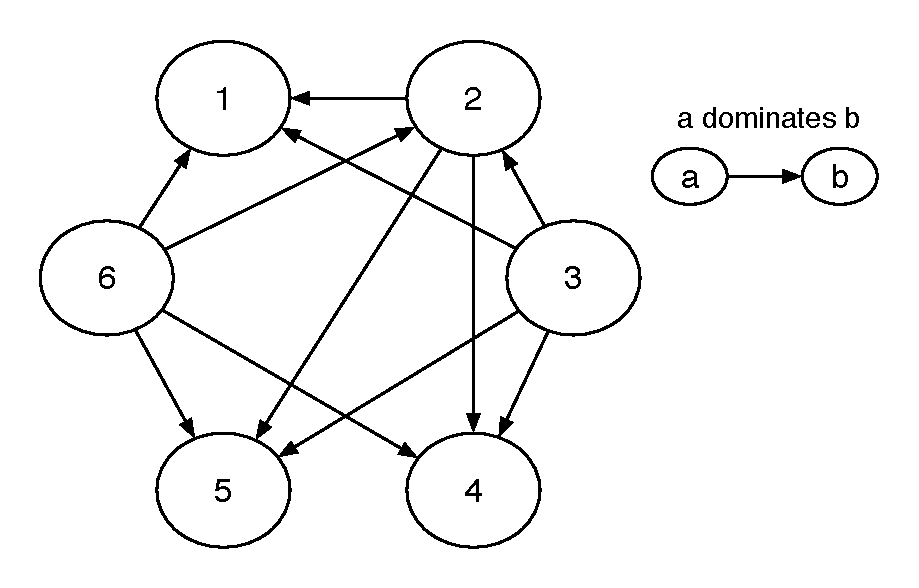
\includegraphics[scale=0.4]{pic/dominance1.eps}
			
		}{%
		\caption{Full Dominance Relationships in Graph}%
	}
	\capbtabbox
	}{%
	\caption{Full Dominance relation in Matrix Form}%
	\label{full_domin}
}
\end{floatrow}
\end{figure}







%\captionlistentry[table]{Full Dominance Relation in Matrix Form}
%\caption{Full Dominance Relation in Graphic and Matrix Forms}


In this example, applicant 2 dominates applicant 1 and applicant 3 dominates
applicant 2, so the dominance between applicant 3 and applicant 1 is redundant
and can be eliminated.

\vspace{0.1in}
\textbf{Redundant Dominance Matrix:}  Graphically, a redundancy relationship
from node $i$ to node $j$ states that there exists at least one two-step path
(not a direct path from node $i$ to node $j$) with one intermediate node, say
from node $i$ to node $k$, and then from node $k$ to node $j$ (where $k$ can be
any intermediate node).  The number of two-step paths from node $i$ to node $j$
with one intermediate node can be easily calculated by
$$ \sum_k d(i,k) \cdot  d(k,j)$$
i.e., if there exists a redundant relationship, the inner product of the two
corresponding vectors should be greater or equal to 1, and 0 otherwise.

The redundancy relationship can thus  be represented in a matrix, denoted as
$D^2$,  as follows. $$D^2 = D^{f} \cdot D^{f} $$  Here $D^f$ is the original
direct dominance matrix and where each entry in $D^2$ represents the number of
two-step paths between a pair of applicants.
 
\textit{Example:} Applicant 2 dominates applicant 1, and applicant 3 dominates
both applicants 1 and 2, therefore the entry $d_{21}=d_{31}=d_{32}=1$. The
relationship between applicant 3 and the other applicants $k$ is:
$d_{3k}=(1,1,0,1,1,0)$, and applicant1 and the other applicants is
$d_{k1}=(0,1,1,0,0,1) ^T $. Furthermore $\sum_k d_{3j} \cdot d_{k1}=d_{31}=1$.
This represents that the relationship between applicants 1 and 3 is redundant.


\begin{figure}
\begin{floatrow}
	\ffigbox{%
		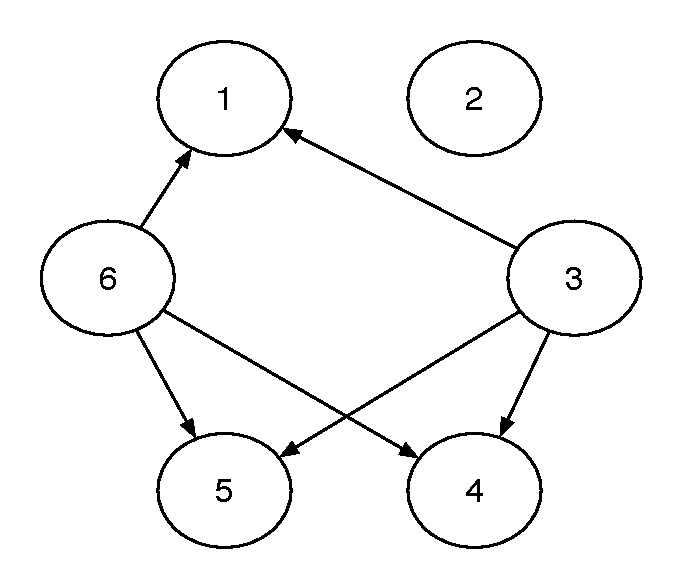
\includegraphics[scale=0.4]{pic/dominance2.eps}
		
	}{%
	\caption{Redundant Dominance Relationships in Graph}%
}
\capbtabbox
}{%
\caption{Redundant Dominance Relation in Matrix}%
\label{redundant1}
}
\end{floatrow}
\end{figure}



Finally, the elements of a \textbf{redundant matrix}, denoted as $ D_r$, can be
defined as follows:
\begin{equation}
d^{r}_{i,j} =
  \begin{cases}
  \quad  1   & \quad if d^{2}_{i,j} >= 1 \\
  \quad  0  & \quad d^{2}_{i,j} = 0 
  \end{cases}	
\end{equation}

\textbf{Minimum cardinality dominance matrix}, defined as $D_m$, can be readily
defined as:
$$D_m = D_f - D_r $$
 
\textit{Example:} By eliminating redundant relationships in the graph, the
minimum dominance graph and matrix forms for the example are presented Figure
\ref{redundant2}:





\begin{figure}
	\begin{floatrow}
		\ffigbox{%
			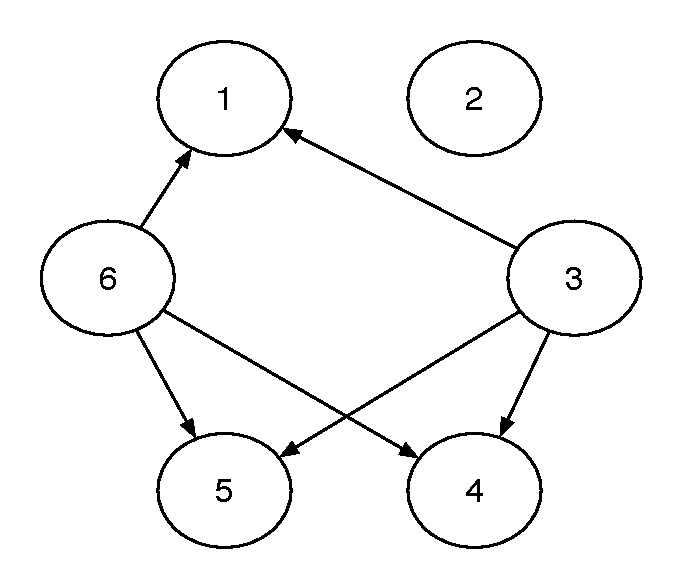
\includegraphics[scale=0.4]{pic/dominance2.eps}
			
		}{%
		\caption{Minimum Dominance in Graph}%
	}
	\capbtabbox
	}{%
	\caption{Minimum Dominance in Matrix}%
	\label{redundant2}
}
\end{floatrow}
\end{figure}


\section{Model Comparison and Results}
Computation experiment shows that the use of minimum cardinality dominance has
achieved a dramatic reduction in terms of model size.  To see this, Table
\ref{model_comparison} presents the numbers of variable and constraints in
respective models. Here though the number of variables has not changed, the
number of constraints has been dramatically reduced, specifically the dominance
constraint (\ref{constraint:2}), which composes the largest part of the model.
The original model has a total of \textbf{13,833,800} dominance constraints due
to the use of direct or full dominance matrix, the reduced model, however, has
only 220,877 constraints.

% Please add the following required packages to your document preamble:
% \usepackage{multirow}
% Please add the following required packages to your document preamble:
% \usepackage{multirow}
\begin{table}[]
\centering
\begin{tabular}{|c|l|c|c|}
\hline
\multicolumn{2}{|c|}{Model Components}                                        &
Original Model & Reduced Model \\ \hline
Variables                   & \multicolumn{1}{|l|}{Allocation (binary)  $x_i$}
& 57,860         & 57,860        \\ \hline
\multirow{3}{*}{Constraint} & One Award per ID  (\ref{constraint:1})        &
5,260          & 5,260         \\ \cline{2-4}
& Dominance  (\ref{constraint:2})               & 13,833,800     & 191,497
\\ \cline{2-4}
& Total Budget   (\ref{constraint:3})           & 1              & 1
\\ \cline{2-4}
& Total Number of Constraints                   & 13,839,061     & 196,758
\\ \hline
\end{tabular}
\caption{Summary of Size of the Optimization Models }
\label{model_comparison}
\label{size_model}
\end{table}

It bears to mention that the solution of the original model with a
state-of-the-art commercial solver is not possible due to memory limitations;
the reduction model, however,  was solved in less than a minute on a standard
laptop computer (30.15 seconds on an Apple Macbook Pro with an i7-4850HQ 2.3
GHz with 16G of RAM).

Table \ref{ssi10k}  presents the solution and the branch and bound process
of the models under various budgets of 2.4M, 2.6M and 2.8M. 
The university has a budget of 2.4M and the solution under that budget is used
in the following analysis.

The computational results under various budgets and SSI are shown in Table
\ref{ssi10k}, Table \ref{ssi12k}, and Table \ref{ssi14k}.
The plots of optimization results are shown in  Figure \ref{ssi_10k_plot},
Figure \ref{ssi_12k_plot} and Figure \ref{ssi_14k_plot}.


When SSI equals to 10000 (Figure \ref{ssi_10k_plot}), 1.2 million budget yield
the maximum revenue. Similarly, when SSI equals to 12000 and 14000, the maximum
revenue reached at 2.2 million and 2.8 million respectively.



%\begin{table}[ht]
%\centering
%\caption{The Integer Programming Solution Process}
%\label{IPSolution}
%\begin{tabular}{|l|l|l|l|l|} \hline
%Linear Programming & Integer Solution & Optimality Gap & Number of Nodes &
%Budget  \\ \hline
%19,212,184.69     & 19,212,039.66    &   0\%            &     80        &
%2.4M\\ \hline
%18,899,616.21   &    18,899,275.7          &    0\%           &     0        &
%2.8M \\ \hline
%\end{tabular}
%\end{table}
%
%


\begin{table}[ht]
\centering
\caption{Computational statistics of optimization model under SSI=10k}
\label{ssi10k}
\begin{tabular}{|c|c|c|c|c|c|}
\hline
SSI                          & \multicolumn{5}{c|}{10000}                      
\\ \hline
\multicolumn{1}{|l|}{Budget} & \multicolumn{1}{l|}{Integer Solution} &
\multicolumn{1}{l|}{Linear Programming} & \multicolumn{1}{l|}{Optimality Gap} &
\multicolumn{1}{l|}{\# Nodes} & \multicolumn{1}{l|}{Time} \\
\hline
0.4M   & 61516543    & 61527360
& 0.02\%    & 0    &27                           \\ \hline
0.6M     & 61552340    & 61559211
& 0.01\%    & 181     &56                        \\ \hline
0.8M   & 61584196    & 61594905
& 0.02\%         & 45         &78                 \\ \hline
1.0M   & 61603302   & 61616648
& 0.02\%     & 0     &27                          \\ \hline
1.2M   & 61624947    & 61625981
& 0.00\%    & 0       &29                         \\ \hline
1.4M      & 61606891    & 61618654
& 0.02\%      & 0          & 108                  \\ \hline
1.6M    & 61593948      & 61602401
& 0.01\%      & 402     &431                      \\ \hline
1.8M       & 61550031         & 61550031
& 0.00\%         & 2270     &1080                 \\ \hline
2.0M       & 61552621       & 61557068
& 0.01\%      & 0          &133                   \\ \hline
2.2M     & 61521260       & 61530258
& 0.01\%    & 0     & 130                         \\ \hline
2.4M   & 61472929   & 61495934
& 0.04\%       & 0   &145                         \\ \hline
2.6M   & 61428352   & 61455128
& 0.04\%     & 80    &410                         \\ \hline
2.8M    & 61414620      & 61416969
& 0.00\%        & 0        &185                   \\ \hline
3.0M    & 61350350     & 61361072
& 0.02\%    & 32    & 209                         \\ \hline
3.2M    & 61260758  & 61272605
& 0.02\%   & 1444      &640                        \\ \hline
3.4M    & 61185830   & 61197559
& 0.02\%   & 598    & 373                          \\ \hline
\end{tabular}
\end{table}




\begin{figure}[ht]
    \centering    
%    [width=5in,height=3.5in,scale=0.5]
    \includegraphics[width=6in,height=2.5in,scale=0.35]{pic/ssi_10k.eps}
    \caption{Optimization results under different budget SSI=10k }
    \label{ssi_10k_plot}
\end{figure}



\begin{table}[ht]
\centering
\caption{Computational statistics of optimization model under SSI=12k}
\label{ssi12k}
\begin{tabular}{|c|c|c|c|c|c|}
\hline
SSI     & \multicolumn{5}{c|}{12000}                      
\\ \hline
\multicolumn{1}{|l|}{Budget} & \multicolumn{1}{l|}{Integer Solution} &
\multicolumn{1}{l|}{Linear Programming} & \multicolumn{1}{l|}{Optimality Gap} &
\multicolumn{1}{l|}{\# Nodes} & \multicolumn{1}{l|}{Time} \\
\hline
1.4M   & 63640276         & 63652166           & 0.02\%         & 230          
& 341  \\ \hline
1.6M   & 63656200         & 63667992           & 0.02\%         & 31           
& 174  \\ \hline
1.8M   & 63647272         & 63647272           & 0.00\%         & 269          
& 280  \\ \hline
2.0M   & 63683212         & 63688055           & 0.01\%         & 0            
& 48   \\ \hline
2.2M   & 63685894         & 63692529           & 0.01\%         & 0            
& 58   \\ \hline
2.4M   & 63676591         & 63688012           & 0.02\%         & 49           
& 159  \\ \hline
2.6M   & 63662739         & 63674086           & 0.02\%         & 78           
& 250  \\ \hline
2.8M   & 63668398         & 63669711           & 0.00\%         & 0            
& 51   \\ \hline
3.0M   & 63620835         & 63640956           & 0.03\%         & 0            
& 61   \\ \hline
3.2M   & 63565618         & 63568716           & 0.00\%         & 1190         
& 806  \\ \hline
3.4M   & 63523681         & 63526856           & 0.00\%          & 529 
& 323  \\ \hline
\end{tabular}
\end{table}



\begin{figure}[ht]
    \centering
%    [width=5in, height=3.5in,scale=0.5]
    \includegraphics[width=5in,height=2.5in,scale=0.3]{pic/ssi_12k.eps}
    \caption{Optimization results under different budget SSI=12k }
     \label{ssi_12k_plot}
\end{figure}




\begin{table}[ht]
\centering
\caption{Computational statistics of optimization model under SSI=14k}
\label{ssi14k}
\begin{tabular}{|c|c|c|c|c|c|}
\hline
SSI     & \multicolumn{5}{c|}{14000}                      
\\ \hline
\multicolumn{1}{|l|}{Budget} & \multicolumn{1}{l|}{Integer Solution} &
\multicolumn{1}{l|}{Linear Programming} & \multicolumn{1}{l|}{Optimality Gap} &
\multicolumn{1}{l|}{\# Nodes} & \multicolumn{1}{l|}{Time} \\
\hline
1.4M    & 65673717     & 65686331
& 0.02\%       & 256    &233                \\ \hline
1.6M   & 65729171  & 65736548
& 0.01\%   & 300     &202                    \\ \hline
1.8M   & 65743219   & 65745436
& 0.00\%       & 1191   & 470                \\ \hline
2.0M  & 65815085   & 65819285
& 0.01\%   & 0  & 107                        \\ \hline
2.2M   & 65844323   & 65855133
& 0.02\%     & 0  & 114                      \\ \hline
2.4M   & 65871923   & 65877439
& 0.01\%     & 2   & 224                     \\ \hline
2.6M      & 65885258     & 65902975
& 0.03\%     & 0       & 124                 \\ \hline
2.8M   & 65919822      & 65923025
& 0.00\%   & 0      & 49                     \\ \hline
3.0M    & 65900599    & 65919720
& 0.03\%   & 0    & 58                       \\ \hline
3.2M  & 65871018    & 65874012
& 0.00\%  & 808    & 451                     \\ \hline
3.4M      & 65857324     & 65887572
& 0.05\%   & 72    & 245                     \\ \hline
\end{tabular}
\end{table}




\begin{figure}[ht]
    \centering
%    [width=5in, height=3.5in,scale=0.5]
    \includegraphics[width=5in,height=2.5in,scale=0.3]{pic/ssi_14k.eps}
    \caption{Optimization results under different budget SSI=14k }
     \label{ssi_14k_plot}
\end{figure}










%\begin{figure}[p] 

\begin{sidewaysfigure}[!htbp]
\centering
\begin{subfigure}{0.33\textwidth}
\includegraphics[width=2.6in,height=2in,scale=0.3]{pic/act_10k.eps}
\caption{} %\label{}
\end{subfigure}\hspace*{\fill}
\begin{subfigure}{0.33\textwidth }
\includegraphics[width=2.6in,height=2in,scale=0.3]{pic/act_12k.eps}
\caption{} %\label{}
\end{subfigure}\hspace*{\fill}
\begin{subfigure}{0.33\textwidth}
\includegraphics[width=2.6in,height=2in,scale=0.3] {pic/act_14k.eps}
\caption{} %\label{}
\end{subfigure}\hspace*{\fill}

\medskip

\begin{subfigure}{0.33\textwidth}
\includegraphics[width=2.6in,height=2in,scale=0.3]{pic/gpa_10k.eps}
\caption{} %\label{}
\end{subfigure}\hspace*{\fill}
\begin{subfigure}{0.33\textwidth }
\includegraphics[width=2.6in,height=2in,scale=0.3]{pic/gpa_12k.eps}
\caption{} %\label{}
\end{subfigure}\hspace*{\fill}
\begin{subfigure}{0.33\textwidth}
\includegraphics[width=2.6in,height=2in,scale=0.3] {pic/gpa_14k.eps}
\caption{} %\label{}
\end{subfigure}\hspace*{\fill}


\medskip

\begin{subfigure}{0.33\textwidth} 
\includegraphics[width=2.6in,height=2.3in]{pic/composite_10k.eps}
\caption{} %\label{}
\end{subfigure}\hspace*{\fill}
\begin{subfigure}{0.33\textwidth }
\includegraphics[width=2.6in,height=2.3in]{pic/composite_12k.eps}
\caption{} %\label{}
\end{subfigure}\hspace*{\fill}
\begin{subfigure}{0.33\textwidth}
\includegraphics[width=2.6in,height=2.3in] {pic/composite_14k.eps}
\caption{} %\label{}
\end{subfigure}\hspace*{\fill}
  \caption{(a) (b) (c) ACT  (d) (e) (f) GPA (g) (h) (i) Composite score}
  \label{allocation_results} 


\end{sidewaysfigure}
%\end{figure}



%
%
%\begin{figure}[ht]
%    \centering
%    \includegraphics[width=5in,height=2.5in,scale=0.3]{pic/act_10k.eps}
%\end{figure}
%
%
%\begin{figure}[ht]
%    \centering
%    \includegraphics[width=5in,height=2.5in,scale=0.3]{pic/act_12k.eps}
%\end{figure}
%
%
%
%\begin{figure}[ht]
%    \centering
%    \includegraphics[width=5in,height=2.5in,scale=0.3]{pic/act_14k.eps}
%\end{figure}
%






\begin{comment}

\subsubsection {Extension with Program Capacity Variations}
University have various units or programs, and typically with various
capacities, that evolve over the years. Proactive marketing and optimization
would help to attract as many students as possible to a business unit with
capacity constraints, or minimal investment for a business unit with excess
capacity (before layoffs or attrition).  The following additional notation is
used in the development of capacity constraints.
\begin{conditions*}
U & &       \quad set of business units under study, indexed by u\\
I_u & &     \quad set of students who are interested in business unit u\\
N_u & &   \quad number of resources (such as faculty members) available for
unit u\\
C_u & &    \quad cost of a single resource\\
\rho_u & & \quad supervising  rate or faculty-to-student ratio for a single
resource in unit u\\
Z_u & &    \quad the additional resource to be hired for each business unit u
\end{conditions*}


\begin{align}
\sum_{i \in I_u}\sum_{m \in M} x_{i,m}\cdot p^e_{i,m}\leq \rho_u\cdot N_u +
\rho_u\cdot Z_u  && \forall u \in U
\end{align}

This constraint states that total number enrolled (left hand size) has to be
less than the current capacity of the program, plus additional hires if
necessary.  The new hires can be added to the objective function.

\end{comment}


\chapter{6. Policy Development \& Implementation}
The results from the optimization specifies the scholarship awards to each
applicant under a specific population and budget.  The actual size and
composition of application poll could be affected by the unemployment rate and
is random in nature.  Nevertheless, at this stage, this study focuses on the
optimization under a specific , etc. poll.  Stochastic optimization techniques
such as sampling will be used to find the optimal allocation under a random
enrichment and is not presented.

\section{Derivation of Financial Aid Policies}
The optimization result based on the above model could be sent to a general
linear regression or decision tree for analysis.  Here the predictor or
dependent variable is the amount of the award and the independent variables are
the variables such as GPA, ACT scores, etc.  However, though it is certain
variables such as Gender could affect the enrollment and graduation
probabilities, thus the final allocation to applicants, awarding scholarship
based on these variables are controversial; as a result, in the derivation of
financial aid policies, certain variables such as gender, family  income, are
not considered in the derivation of a merit-based scholarship.

 \subsection{Financial Aid Policy Based on Decision Tree }
The decision tree analysis is used in the derivation of the financial aid
policy.  In the past two decades, decision trees, as a decision support tool,
have been commonly used in various business domains, such as direct mailing,
online sales, customer retention and supplier selection, to name a few
\citep{Han2011}.













Decision tree analysis is a tree-structure model to structure  in which each
internal node represents a ``test" on an attribute, each branch represents the
outcome of the test and each leaf node represents a class label (decision taken
after computing all attributes). The paths from root to leaf represents
classification rules.  The financial aid policy from the decision tree analysis
is presented in Figure \ref{FApolicybyDT}.
 
  
 
\begin{sidewaysfigure}
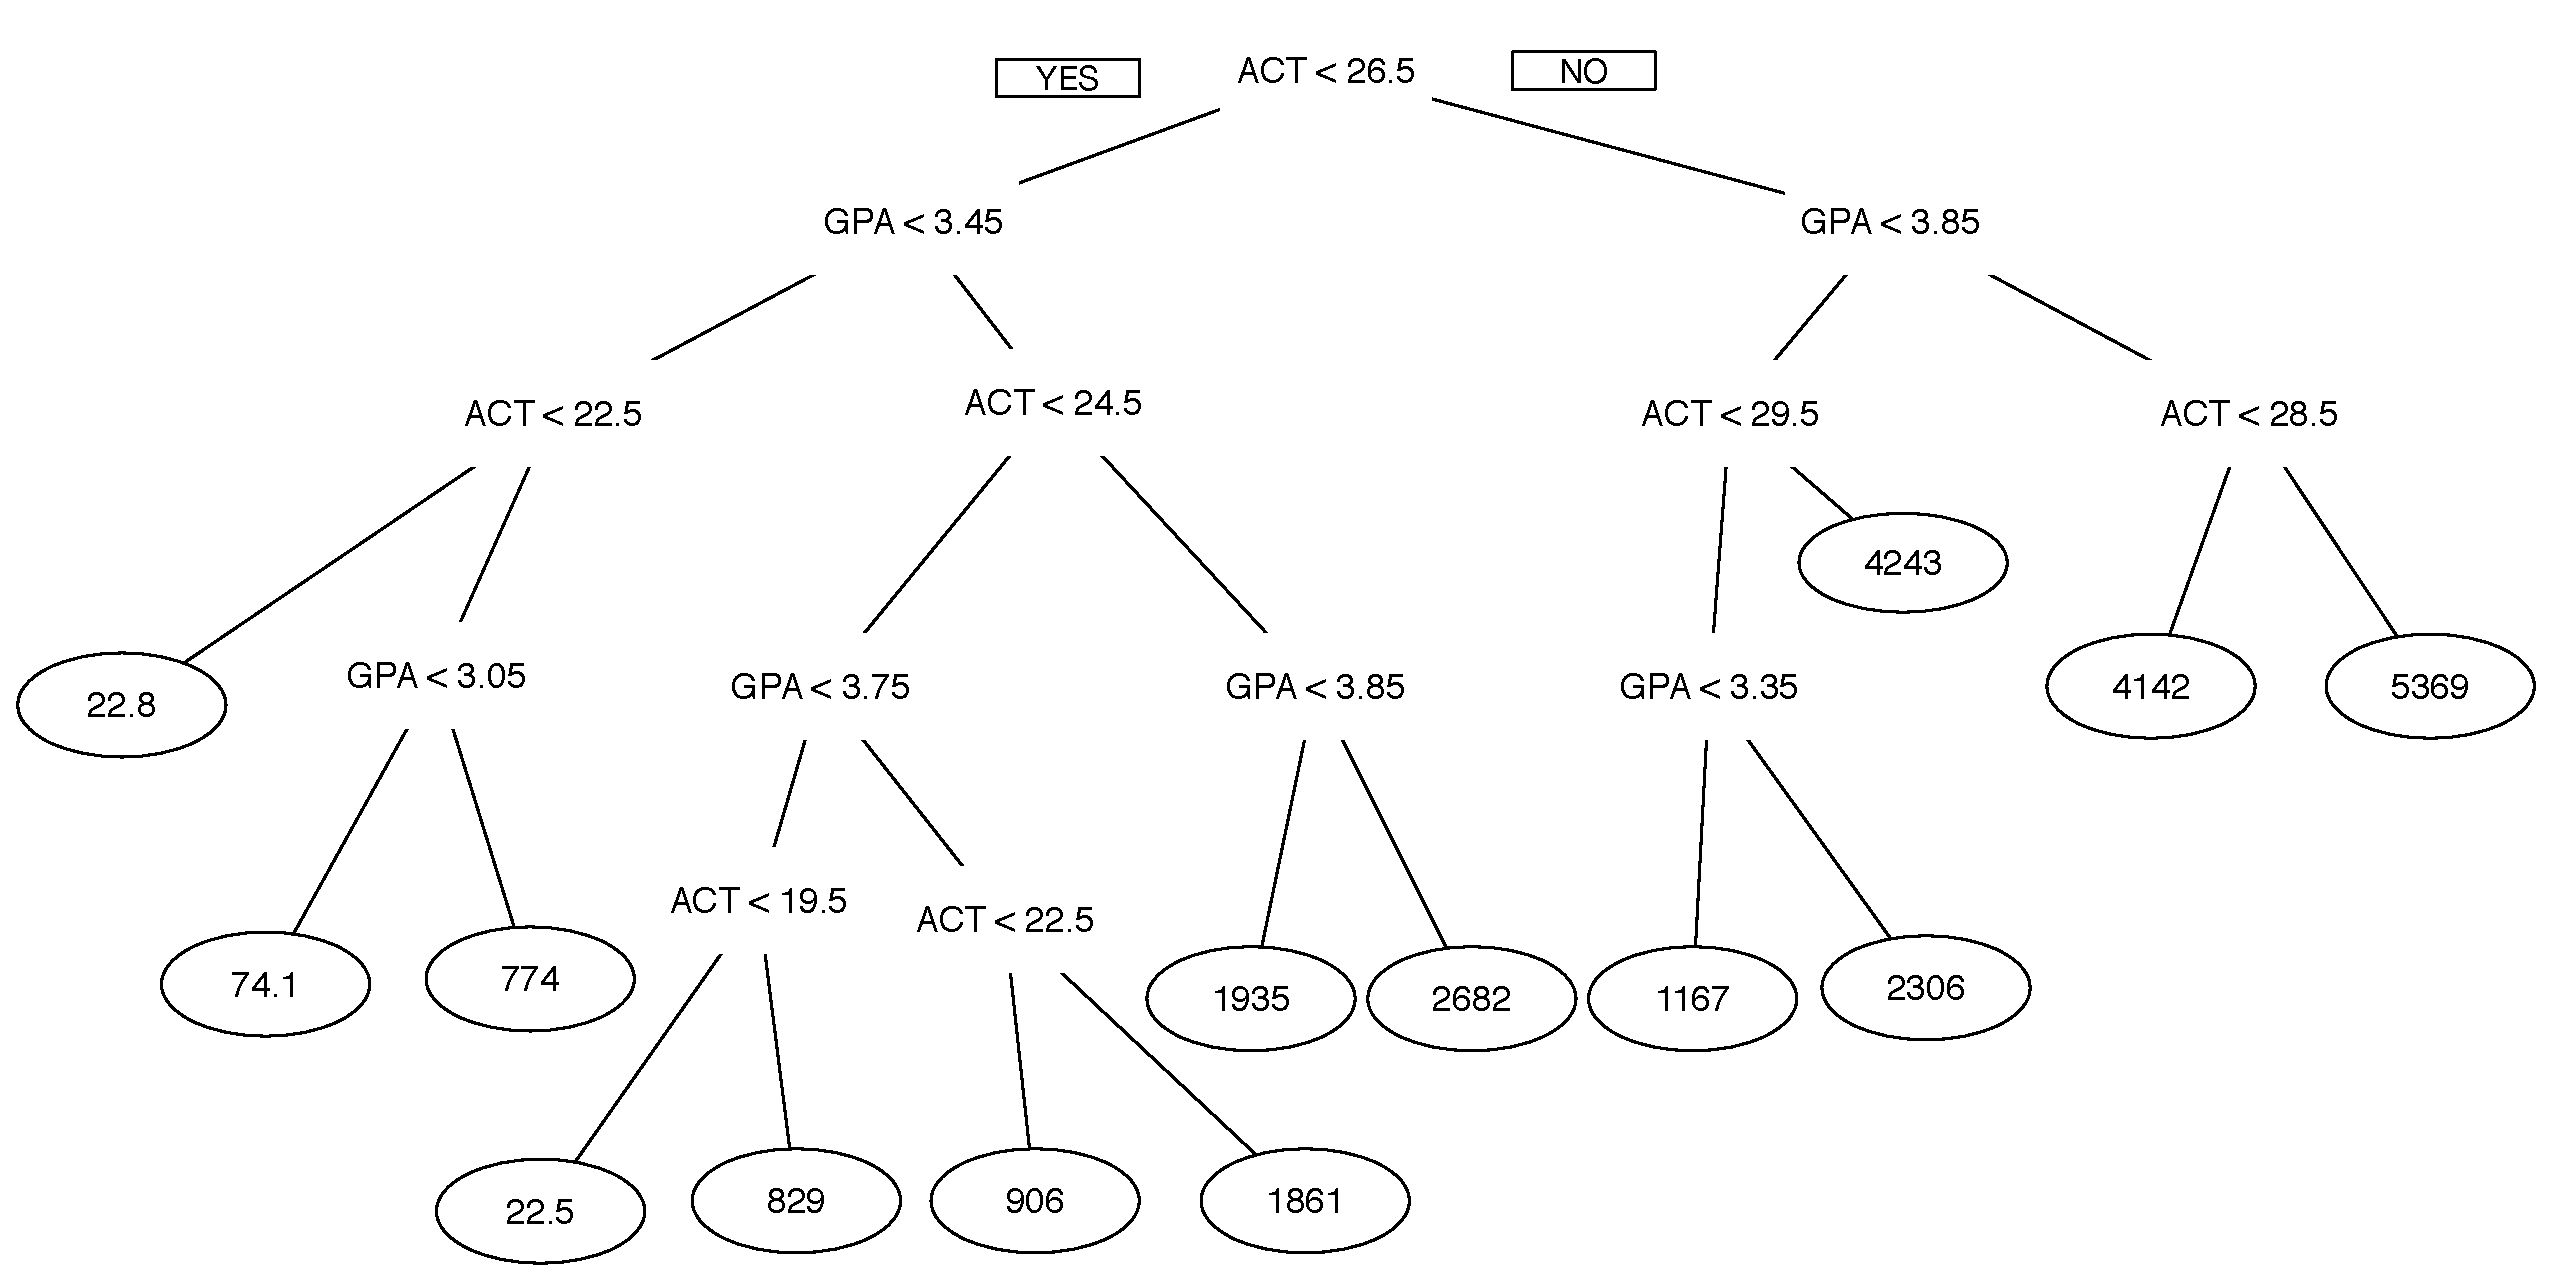
\includegraphics[width=7in, height=5in]{pic/FA_DT_Result.eps}%
\caption{Financial Aid Policy Based on Decision Tree }
\label{FApolicybyDT}
\end{sidewaysfigure}
 
%\end{landscape}

% 
%todo The Policy reads as follows:  If the applicants xxxxxxxxxxxxxxxxxxxxxxx

\subsection{A Simple Financial Aid Policy Base on Stepwise Regression}
The decision tree analysis, though graphical, still seems a little complicated.
To reveal more intuitive answer to the financial aid from the optimization
results, Table \ref{opt_scholar_act} presents the average financial aid with
respect to the students' GPA and ACT scores. Here the row names represents the
GPA scores, and the column names represent the ACT scores. The average
financial aid awarded (of the optimal results with a budget of 2.8 million
scholarship) is shown in the corresponding grid.

\begin{sidewaystable}[!htbp]
 \resizebox{\linewidth}{200pt}{
\begin{tabular}{@{\extracolsep{5pt}} |l|cccccccccccccccccc|c|}
\hline
GPA/ACT  & \multicolumn{1}{c|}{18}     & \multicolumn{1}{c|}{19}
& \multicolumn{1}{c|}{20}          & \multicolumn{1}{c|}{21}          &
\multicolumn{1}{c|}{22}          & \multicolumn{1}{c|}{23}   &
\multicolumn{1}{c|}{24}          & \multicolumn{1}{c|}{25}          &
\multicolumn{1}{c|}{26}        & \multicolumn{1}{c|}{27}         &
\multicolumn{1}{c|}{28}          & \multicolumn{1}{c|}{29}          &
\multicolumn{1}{c|}{30}          & \multicolumn{1}{c|}{31}         &
\multicolumn{1}{c|}{32}          & \multicolumn{1}{c|}{33}          &
\multicolumn{1}{c|}{34}          & 35     & Total \\ \hline
1           &                                  &
&                                  &                                  &     &
&                                  &                                  &     &
&                                  &                                  &
&                                 &                                  &
&                                  &        & 0           \\ \cline{1-1}
\cline{20-20}
1.1         &                                  &
&                                  &                                  &
&                           &                                  &
&                                &                                 &
&                                  &                                  &
&                                  &                                  &
&        & 0           \\ \cline{1-1} \cline{20-20}
1.2         &                                  & 0
&                                  &                                  &
&                           &                                  &
&                                &                                 &
&                                  &                                  &
&                                  &                                  &
&        & 0           \\ \cline{1-1} \cline{20-20}
1.3         & 0                                &
&                                  &                                  &
&                           &                                  &
&                                &                                 &
&                                  &                                  &
&                                  &                                  &
&        & 0           \\ \cline{1-1} \cline{20-20}
1.4         &                                  & 0
&                                  &                                  &
&                           &                                  &
&                                &                                 &
&                                  &                                  &
&                                  &                                  &
&        & 0           \\ \cline{1-1} \cline{20-20}
1.5         &                                  & 0
&                                  &                                  &
&                           &                                  &
& 0                              &                                 &
&                                  &                                  &
&                                  &                                  &
&        & 0           \\ \cline{1-1} \cline{20-20}
2.5         & 0                                & 0
& 0                                & 0                                & 0
& 0                         & 0                                & 0
& 0                              & 0                               & 0
& 0                                &                                  & 0
&                                  &                                  &
&        & 0           \\ \cline{1-1} \cline{20-20}
2.6         & 0                                & 0
& 0                                & 0                                & 0
& 0                         & 0                                & 0
& 0                              & 0                               &
& 1250                             & 1500                             &
&                                  & 1500                             &
&        & 25.8 \\ \cline{1-1} \cline{20-20}
2.7         & 0                                & 0
& 0                                & 0                                & 0
& 0                         & 0                                & 0
& 0                              & 0                               & 1500
&                                  & 2000                             &
&                                  &                                  &
&        & 24.2 \\ \cline{1-1} \cline{20-20}
2.8         & 0                                & 0
& 0                                & 0                                & 0
& 0                         & 0                                & 0
& 0                              & 300                             & 1500
& 2000                             &                                  &
&                                  & 2500                             &
&        & 39.4 \\ \cline{1-1} \cline{20-20}
2.9         & 0.0                              & 0.0
& 0.0                              & 0.0                              & 0.0
& 0.0                       & 0.0                              & 0.0
& 818.2                          & 1875.0                          & 2000.0
&                                  &                                  &
&                                  &                                  &
&        & 63.4        \\ \cline{1-1} \cline{20-20}
3           & 0.0                              & 0.0
& 0.0                              & 0.0                              & 0.0
& 0.0                       & 0.0                              & 1166.7
& 1500.0                         & 2000.0                          & 2000.0
& 2200.0                           &                                  & 3200.0
&                                  &                                  & 5200.0
&        & 216.3       \\ \cline{1-1} \cline{20-20}
3.1         & 0.0                              & 0.0
& 0.0                              & 0.0                              & 0.0
& 0.0                       & 523.8                            & 1500.0
& 1727.3                         & 2000.0                          & 2000.0
& 2500.0                           & 2500.0                           &
&                                  &                                  &
& 7300.0 & 276.7       \\ \cline{1-1} \cline{20-20}
3.2         & 0.0                              & 0.0
& 0.0                              & 0.0                              & 0.0
& 781.3                     & 1000.0                           & 1750.0
& 2000.0                         & 2250.0                          & 2500.0
& 2500.0                           & 2780.0                           & 3950.0
& 5200.0                           &                                  &
&        & 573.7       \\ \cline{1-1} \cline{20-20}
3.3         & 0.0                              & 0.0
& 0.0                              & 0.0                              & 647.1
& 1000.0                    & 1613.6                           & 2000.0
& 2315.8                         & 2500.0                          & 2920.0
& 3200.0                           & 3866.7                           & 4200.0
&                                  & 5200.0                           & 5200.0
&        & 962.8       \\ \cline{1-1} \cline{20-20}
3.4         & 0.0                              & 0.0
& 0.0                              & 694.4                            & 1000.0
& 1550.0                    & 2000.0                           & 2000.0
& 2500.0                         & 2990.0                          & 3200.0
& 3200.0                           & 4200.0                           & 4200.0
&                                  &                                  &
&        & 1185.1      \\ \cline{1-1} \cline{20-20}
3.5         & 0.0                              & 0.0
& 695.7                            & 1000.0                           & 1724.1
& 2000.0                    & 2000.0                           & 2216.7
& 2500.0                         & 3200.0                          & 3200.0
& 3200.0                           & 4200.0                           & 4200.0
&                                  & 5200.0                           &
&        & 1696.7      \\ \cline{1-1} \cline{20-20}
3.6         & 0.0                              & 545.5
& 1000.0                           & 1000.0                           & 2000.0
& 2000.0                    & 2357.1                           & 2500.0
& 2864.0                         & 3200.0                          & 3200.0
& 3800.0                           & 4200.0                           & 4200.0
& 5200.0                           & 5200.0                           & 5200.0
&        & 2148.1      \\ \cline{1-1} \cline{20-20}
3.7         & 0.0                              & 1000.0
& 1000.0                           & 1500.0                           & 2000.0
& 2285.7                    & 2500.0                           & 2945.5
& 3200.0                         & 3200.0                          & 3700.0
& 4200.0                           & 4200.0                           & 5200.0
& 5200.0                           &                                  & 5200.0
&        & 2532.8      \\ \cline{1-1} \cline{20-20}
3.8         & 0.0                              & 1000.0
& 1000.0                           & 2000.0                           & 2000.0
& 2500.0                    & 3006.9                           & 3200.0
& 3200.0                         & 4014.8                          & 4200.0
& 4200.0                           & 4900.0                           & 5200.0
& 5200.0                           & 5200.0                           &
&        & 3007.5      \\ \cline{1-1} \cline{20-20}
3.9         & 666.7                            & 1000.0
& 1000.0                           & 2000.0                           & 2000.0
& 2500.0                    & 3200.0                           & 3200.0
& 3680.0                         & 4200.0                          & 4200.0
& 4644.4                           & 5200.0                           & 5200.0
& 5200.0                           & 5200.0                           & 5200.0
&        & 3360.4      \\ \cline{1-1} \cline{20-20}
4           &                                  & 1000.0
& 1000.0                           & 2000.0                           & 2000.0
& 2500.0                    & 3200.0                           & 3200.0
& 4200.0                         & 4808.7                          & 5200.0
& 5200.0                           & 5200.0                           & 5200.0
& 5200.0                           & 5200.0                           & 6542.9
& 7300.0 & 4186.1      \\ \cline{1-1} \cline{20-20}
4.1         &                                  & 1000.0
& 1000.0                           & 2000.0                           & 2000.0
& 2500.0                    & 3200.0                           & 3200.0
& 4200.0                         & 5200.0                          & 5200.0
& 5200.0                           & 5200.0                           & 5200.0
& 5200.0                           & 5200.0                           & 7300.0
&        & 3982.1      \\ \cline{1-1} \cline{20-20}
4.2         & 1000.0                           &
& 1000.0                           & 2000.0                           & 2000.0
& 2500.0                    & 3200.0                           & 3200.0
& 4200.0                         & 5200.0                          & 5200.0
& 5200.0                           & 5200.0                           & 5200.0
& 5200.0                           & 5200.0                           & 7300.0
&        & 4175.0      \\ \cline{1-1}
4.3         &                                  &
&                                  &                                  & 2000.0
& 2500.0                    & 3200.0                           & 3200.0
& 4200.0                         & 5200.0                          & 5200.0
& 5200.0                           & 5200.0                           & 5200.0
& 5200.0                           & 5200.0                           & 7300.0
&        & 4607.9      \\ \cline{1-1} \cline{20-20}
4.4         &                                  &
&                                  &                                  &
&                           & 3200.0                           & 4200.0
& 5200.0                         & 5200.0                          & 5200.0
& 5200.0                           & 5200.0                           & 5200.0
& 5200.0                           & 5200.0                           & 7300.0
&        & 5125.0      \\ \cline{1-1} \cline{20-20}
4.5         &                                  &
& 1000.0                           &                                  & 2000.0
& 2925.0                    &                                  & 5200.0
& 5200.0                         &                                 & 5200.0
& 5200.0                           &                                  & 5200.0
& 5200.0                           & 6233.3                           &
& 7300.0 & 4605.3      \\ \cline{1-1} \cline{20-20}
4.6         &                                  &
&                                  &                                  &
& 4200.0                    &                                  &
& 5200.0                         & 5200.0                          & 5200.0
&                                  & 5200.0                           &
& 5900.0                           & 7300.0                           & 7300.0
&        & 5730.0      \\ \cline{1-1} \cline{20-20}
4.7         &                                  &
&                                  & 5200.0                           &
&                           &                                  &
& 5200.0                         & 5200.0                          & 6200.0
&                                  &                                  & 8400.0
& 8400.0                           & 8400.0                           &
&        & 6377.8      \\ \cline{1-1} \cline{20-20}
4.8         &                                  &
&                                  &                                  &
&                           &                                  &
&                                & 5200.0                          & 6200.0
&                                  & 6200.0                           &
&                                  &                                  &
&        & 5866.7      \\ \hline
Grand Total & \multicolumn{1}{c|}{7.2} & \multicolumn{1}{c|}{92.7} &
\multicolumn{1}{c|}{166.2} & \multicolumn{1}{c|}{428.7} &
\multicolumn{1}{c|}{787.1} & \multicolumn{1}{c|}{1206} &
\multicolumn{1}{c|}{1664.8} & \multicolumn{1}{c|}{2112} &
\multicolumn{1}{c|}{2642.1} & \multicolumn{1}{c|}{3407.5} &
\multicolumn{1}{c|}{3835.6} & \multicolumn{1}{c|}{3981.3} &
\multicolumn{1}{c|}{4561.4} & \multicolumn{1}{c|}{4784.9} &
\multicolumn{1}{c|}{5323.2} & \multicolumn{1}{c|}{5258.8} &
\multicolumn{1}{c|}{6247.6} & 7300   & 1134.7 \\ \hline
\end{tabular}}
\caption{Optimization Mean Scholarship vs GPA and ACT}
\label{opt_scholar_act}
\end{sidewaystable}

These results clearly suggest a strong relationship between the awards and both
GPA and ACT scores.  As a result, a \textit{composite score} index, calculated
as $10 \times GPA + ACT $ was proposed by the enrollment team to capture the
applicants academic merits and used as the basis of the award.

Figure \ref{compositescore} presents the average award from the optimization
results for the composite score. Here, the horizontal axis represents the
composite score and the vertical axis the average scholarship awarded for the
corresponding score.
 \begin{figure}[ht]
   \centering
 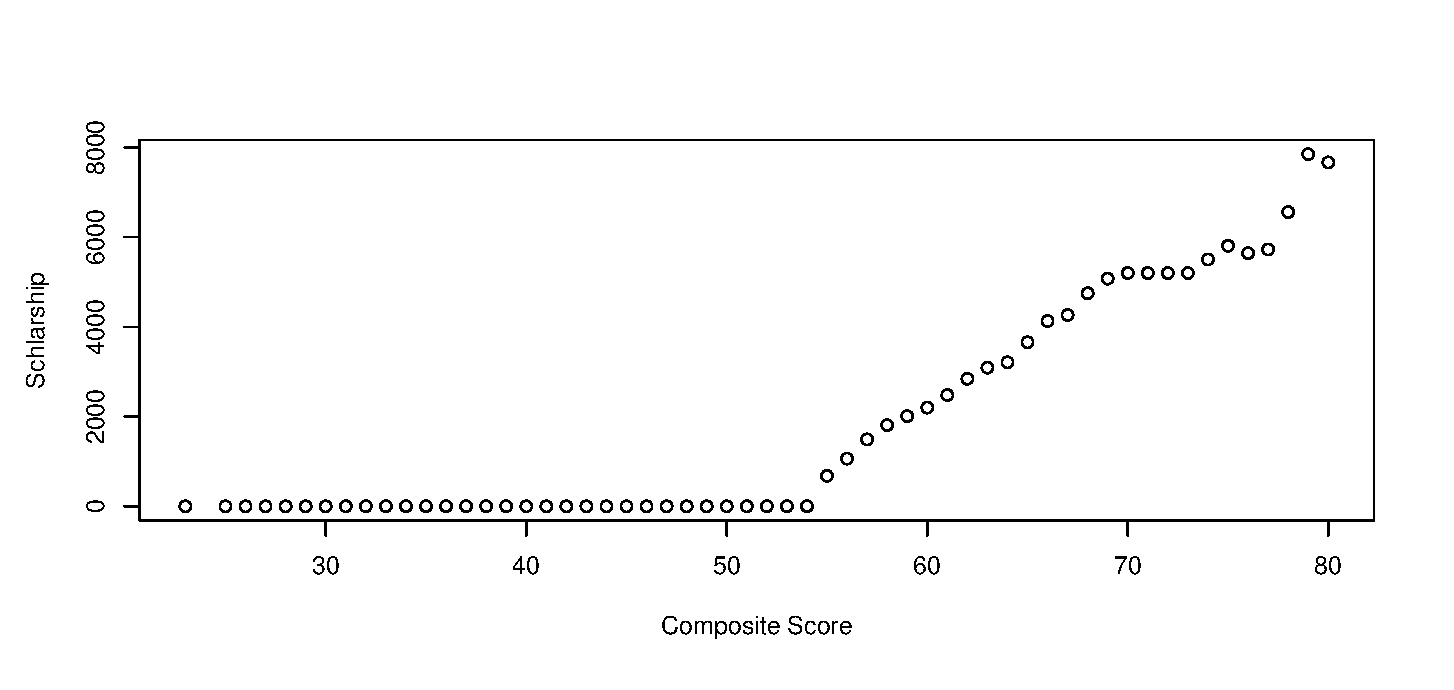
\includegraphics[scale=0.65]{pic/scho_composite.eps}
 \caption{Scholarship versus composite score}
 \label{compositescore}
\end{figure}

The figure clearly shows that no scholarship should be awarded when the
combined score is below 54.  A linear relationship seems to exist between the
scholarship and the composite score when the composite score is between 55 and
70, and the scholarship seems to remain the same when the score is above 70.
Use ``CS'' as the variable representing the composite score, a piecewise
regression is used to capture these observations and the resulting regression
equations are shown in Table \ref{money_result} and a graph of the piecewise
regression is shown in \ref{AppB}. A simpler discretized version of the
scholarship policy is shown in Table \ref{money_result_discrete}.

\begin{table}[ht]
\centering
\begin{tabular}{|c|c|c|}
\hline
Composite Score & \# of Applicants & Scholarship Amount \\ \hline
0-53.9         & 2,897	&0              \\ \hline
54-68.9        & 2,103  &$309\times CS -16,380 $            \\ \hline
69-76.9        &  241 &  $101\times CS - 2,024$           \\ \hline
77-80       & 19 &   $711 \times CS -48,910$          \\ \hline
\end{tabular}
\caption{Piecewise Scholarship Allocation}
\label{money_result}
\end{table}


\begin{table}[ht]
\centering
\begin{tabular}{|c|c|}
\hline
Composite Score & Scholarship Amount \\ \hline
0-54.9         & 0              \\ \hline
55-59.9         & 1,500              \\ \hline
60-65.9         & 2,500              \\ \hline
66-69.9         & 3,500              \\ \hline
70-74.9         & 4,500              \\ \hline
75+             & 6,000              \\ \hline
\end{tabular}
\caption{Discretized Version of Scholarship Allocation}
\label{money_result_discrete}

\end{table}

\begin{comment}
\subsection{Comparison of Policies} 

Feeding Back these policies into the optimization model, table
\ref{policy_compare} presents the results of various policies. Here  the
Objective column represents the objective values, Enrollment represents the
expected enrollment; the graduation represents the expected number of
graduation; tuition represents the expected tuition income, and SSI represents
the expected SSI from state when applicant enroll and graduate.



	
\begin{table}[]
\centering
\caption{My caption}
\label{my-label}
\begin{tabular}{|l|l|l|l|l|l|} \hline
Policy                        & Objective & Enrollment & Graduation& Tuition &
SSI  \\ \hline \hline
Optimization Result &                 &                   &                   &
&                     \\ \hline
Decision Tree Model  &                 &                   &
&                  &                     \\ \hline
Stepwise Regression Model     &                 &                   &
&                  &                     \\ \hline
Discrete Stepwise Regression  &                 &                   &
&                  &                     \\ \hline
Current Policy                &                 &                   &
&                  &                    \\ \hline
\end{tabular}
\label{policy_compare}
\end{table}

As can be seen, it s expected that a 10\% increase in enrollment from *** to **
if we adopted the optimal result and perform individualize scholarship.  DT
tree analysis and stepwise regression and discrete stepwise regression based on
composite scores ********

Out of the composite scores, DT preforms best , followed by Stepwise 
\end{comment}


\section{Implementation and Results}
The scholarship allocation based on the composite score and the policy
presented in Table \ref{money_result} has been used as the foundation for the
scholarship for the university in the 2013 to 2014 academic year.  A proactive
approach has been taken by the university. The enrollment and admission office
has purchased data on student performance and  scholarship awards before they
even apply (these awards hinge upon the verification of their official
performance). For details, please see
\url{http://www.wright.edu/raider-connect/financial-aid/first-year-scholarships
}.


Table \ref{enroll_stats} presents the enrollment statistics for the university
in the 2012 - 2013 academic year and those of the 2013 - 2014 academic year.

\begin{table}[ht!]
\centering
\begin{tabular}{|c|c|c|c|c|}
\hline
& 2013 & 2014 & \# Increase & \% Increase \\ \hline
Application                    & 6,101 & 6,068 & -43         & -0.7\%      \\
\hline
Admitted                       & 4,541 & 4,773 & 232         & 5.1\%       \\
\hline
Non-Scholarship                & 2,166 & 2,157 & -9          & -0.4\%      \\
\hline
Scholarship Award              & 2,375 & 2,616 & 241         & 10.1\%      \\
\hline
%\% of scholarship              & 52\% & 55\% &             &             \\
%\hline
Matriculated                   & 2,001 & 2,222 & 221         & 11.0\%      \\
%\hline
%Non-Scholarship Student        & 931  & 1000 & 69          & 7.4\%       \\
%\hline
%Scholarship Student            & 1070 & 1222 & 152         & 14.2\%      \\
%\hline
%Scholarship Matriculation Rate & 45\% & 47\% &             &             \\
\hline
\end{tabular}
\caption{Enrollment Statistics for the 2012-2013 and 2013-2014 Academic Years}
\label{enroll_stats}

\end{table}

In 2012-2013, there are a total of 6,101 applicants, of them,4,541   are
admitted. 2,375 were awarded scholarships and 2,166 were not scholarships. 52\%
of the students were awarded scholarships, and a total of 2,001 students
matriculated.

In the 2013-2014 academic year, there were a total of 6,068 applicants; of
them, 4,773 were admitted, 2,616 were awarded scholarships and 2,157 were not
awarded scholarships, 56\% of the students are awarded scholarships and a total
of 2,222 students matriculated.

Notice that the number of applicants does not change dramatically, actually
showing a reduction of -43 (-0.7\% increase), but the actual enrollment
increased by 221  or 11.0\% over the previous years.  It is believed that the
use of the optimal policy could generate millions of dollars or in revenue for
the university in the next few years.


\begin{comment}
\section{Time Line}

Several tasks need to be completed in the remaining year and the intended
graduation and thesis defense is August 2017.  These tasks and time lines are
presented in Table \ref{timeline}.

\begin{table}[ht]
\centering

\begin{tabular}{|l|l|}
\hline
Tasks                                                                & Time
Line \\ \hline
Development and Comparison of Other Prediction Methods               &  9/2016
\\ \hline
Optimization Result Comparison of Various Budget Constraints          & 10/2016
\\ \hline
Optimization Result Under Different Applications Pool			 &       11/2016
\\ \hline
Finish Writing Papers and Submit Thesis                             		&  2/2017
\\ \hline
\end{tabular}
\caption{Future Study}
    \label{timeline}
\end{table}
\end{comment}


\begin{comment}
\section{Implementation}


In an attempt to improve the academic profile of our new, direct from high
school class of all 2013 and to address capacity for growth within the
colleges, the  financial aid office did a study: WSU awarded additional
scholarship funds to students who were direct admits into some colleges. The
students targeted had an average HS GPA of 3.97 and an ACT of 27+. Overall this
funding proved to be very successful because the number of students who
enrolled with a HS GPA of 4.0 and greater increased by 51\% and the students
who had an ACT of 31+ increased by 18\%. WSU matriculated an additional 34\% of
students in this group due to the additional funding.
%This effort began our scholarship leveraging efforts, and we had good results
considering the timing of the original project.
    	
After an extensive data review process, we found that because the average award
for this group of students increased to \$3,500-\$4,500 (full in-state tuition
is \$8,354), WSU were able to attract higher achieving students with the
additional scholarships, by meeting their `need'\ for competitive merit-based
scholarships. WSU were competitive with our peers by percentage of tuition
discounted for this group.

We initiated the study in the 2013 Fall semester to redesign our merit-based
scholarship structure aiming to increase the headcount without sacrificing
academic profile. At the same time, a massive marketing campaign lead by the
school administration kicked off. Since more than 95\% of the incoming students
at WSU are Ohio residents, our study is focus on this group of students.

Application data from 2006 to 2013 was collected via the enrollment office. The
data contains mainly two categories: students academic profiles and economic
status. More details are included in the study approach portion of this study.
\end{comment}

% Study on enrollment management falls into two main areas
\citet{Maltz2007}: developing predicting models for enrollment levels and
on systems for identifying expected targeting applicants. And the prediction
models largely consist of two levels \citet{Aksenova2006}: (1)
curve-fitting techniques such as moving averages, exponential smoothing,
spectral analysis; (2) data mining models such as regression models, tree
structure models, stochastic models.

\chapter{Conclusion}

\appendix
\chapter{Appendix A: Summary Statistics of Data Fields Provided by the
University}  \label{app A}

%\section{Variables used in the model}

The variable used in the model contains both continuous and discrete variables
and are listed in the table below.

 
\begin{sidewaystable*}
%\begin{table}[]
\centering

\caption{Summary of categorical variables}
\label{enroll_discrete}
\begin{adjustbox}{width=1.05\textwidth}

\begin{tabular}{lccccl}
\\[-1.8ex]\hline 
\hline
Variable                        & Enrolled & Not Enrolled & Graduated & Not
Graduated & Definitions of Variables                    \\ \hline
Tier 1                          & 7190    & 6322        & 1471     & 5719      
& Dummy; 1=Tier 1; 0=otherwise                \\ 
Tier 2                          & 2183    & 2909        & 438       & 1745     
& Dummy; 1=Tier 2; 0=otherwise                \\
Tier 3                          & 606      & 672          & 179       & 427    
& Dummy; 1=Tier 3; 0=otherwise                \\
Tier 4                          & 2146    & 4446        & 243       & 1903     
& Dummy; 1=Tier 4; 0=otherwise                \\
Tier 5                          & 1145    & 2620        & 242       & 903      
& Dummy; 1=Tier 5; 0=otherwise                \\
Tier 6                          & 1943    & 3149        & 441       & 1502     
& Dummy; 1=Tier 6; 0=otherwise                \\
Asian                           & 319      & 378          & 76        & 243    
& Dummy; 1=Asian; 0=otherwise                 \\
African American                & 2916    & 4400        & 264       & 2652     
& Dummy; 1=African American; 0=otherwise      \\
Hawaiian                        & 15       & 15           & 1         & 14     
& Dummy; 1=Hawaiian; 0=otherwise              \\
Hispanic                        & 355      & 461          & 57        & 298    
& Dummy; 1=Hispanic; 0=otherwise              \\
Native Indian/Alaskan           & 36       & 39           & 8         & 28     
& Dummy; 1=Native Indian/Alaskan; 0=otherwise \\
Two/More                        & 504      & 454          & 78        & 426    
& Dummy; 1=Two/More; 0=otherwise              \\
Unknown                         & 118      & 451          & 22        & 96     
& Dummy; 1=Unknown ; 0=otherwise              \\
White                           & 10949   & 13917       & 2508      & 8441     
& Dummy; 1=White; 0=otherwise                 \\
College of Business (BA)        & 1636    & 2167        & 375       & 1261     
& Dummy; 1=BA; 0=otherwise                    \\
College of Science \& Math (SM) & 2330    & 2931        & 491       & 1839     
& Dummy; 1=SM; 0=otherwise                    \\
College of Liberal Arts (LA)    & 2714    & 3976        & 527       & 2187     
& Dummy; 1=LA; 0=otherwise                    \\
College of Education (ED)       & 1419    & 1973        & 284       & 1135     
& Dummy; 1=ED; 0=otherwise                    \\
College of Engineering (EG)     & 2081    & 2347        & 482       & 1599     
& Dummy; 1=EG; 0=otherwise                    \\
College of Nursing (N)          & 2033    & 2675        & 337       & 1696     
& Dummy; 1=N; 0=otherwise                     \\
University College  (UC)        & 3000    & 4049        & 518       & 2483     
& Dummy; 1=UC; 0=otherwise                    \\
Female                          & 9922    & 10784       & 1816  & 6936  &
Dummy; 1=Female; 0=otherwise  \\
Male                            & 7270    & 7367        & 1198      & 5263   &
Dummy; 1=Male;0=otherwise    \\
Underrepresented-Yes            & 4146    & 5748        & 483       & 3662     
& Dummy; 1=Underrepresented; 0=otherwise      \\
Underrepresented-No             & 11067   & 14370       & 2530      & 8537     
& Dummy; 1=Not Underrepresented ; 0=otherwise\\
Raider County         & 10299   & 10404   & 2160        &  8139     & Dummy;
1=Raider (County close to WSU); 0=otherwise                     \\
Not Raider County  & 4914       & 9714     & 854       & 4060        & Dummy;
1=NotRaider (County not close to WSU) ; 0=otherwise   \\
 \hline 
\end{tabular}
\end{adjustbox}
%\end{table}
\end{sidewaystable*}



\begin{sidewaystable*}{}
\centering
\caption{Summary of continuous variables}
\label{continuous}

\begin{adjustbox}{width=1.05\textwidth}
\begin{tabular}{lccccccl}
\\[-1.8ex]\hline
\hline 
Variable          & n        & mean        & sd          & median   & min      
& max       & Description of Variables                                         

\\ \hline
GPA                & $35331$ & $3.094$     & $0.63$     & $3.10$  & $0.40$    
& $4.90$   & High School GPA \\
ACT                & $35331$ & $21.268$    & $4.39$     & $21$     & $8$    &
$36$   & Composite ACT   \\
HS PERCENTILE      & $35331$ & $60.89$    & $24.83$    & $64$     & $0$        
& $100$     & Hight School Percentile Rank                                     
\\
SCHOLARSHIP        & $35331$ & $777.45$   & $1339.30$ & $0$      & $0$        
& $8354$   & Scholarship offered                                               
\\
PELL GRANT         & $35331$ & $1452.15$ & $2228.13$ & $0$      & $0$         &
$5550$   & Pell Grant Information \\
TOTAL FREE MONEY   & $35331$ & $2229.61$ & $2492.47$ & $150$  & $0$         &
$1390$  & SCHOLARSHIP + PELL GRANT                                             
\\
OUT OF POCKET      & $35331$ & $5455.20$ & $2467.15$ & $6278$  & $$-$5935$ &
$8354$   & TUITION - TOTAL FREE Money                                          
\\
DISTANCE.NUM       & $35331$ & $57.67$    & $53.49$    & $43.82$ & $2.65$     &
$276.75$ & \begin{tabular}[c]{@{}l@{}}Distance between high school \\ to WSU
main campus\end{tabular} \\
UNEMPLOYMENT.INDEX & $35331$ & $7.91$     & $1.890$     & $7.400$  & $5.40$    
& $10.40$  & \begin{tabular}[c]{@{}l@{}}Unemployment rate of \\ application
year\end{tabular}           \\
COMB SCORE  & $35331$ & $52.20$  & $9.60$  & $52$  & $21$   & $82$  & GPA * 10
+ ACT    \\   
\hline
\end{tabular}
\end{adjustbox}
\end{sidewaystable*}








\begin{figure}[ht]
   \centering
 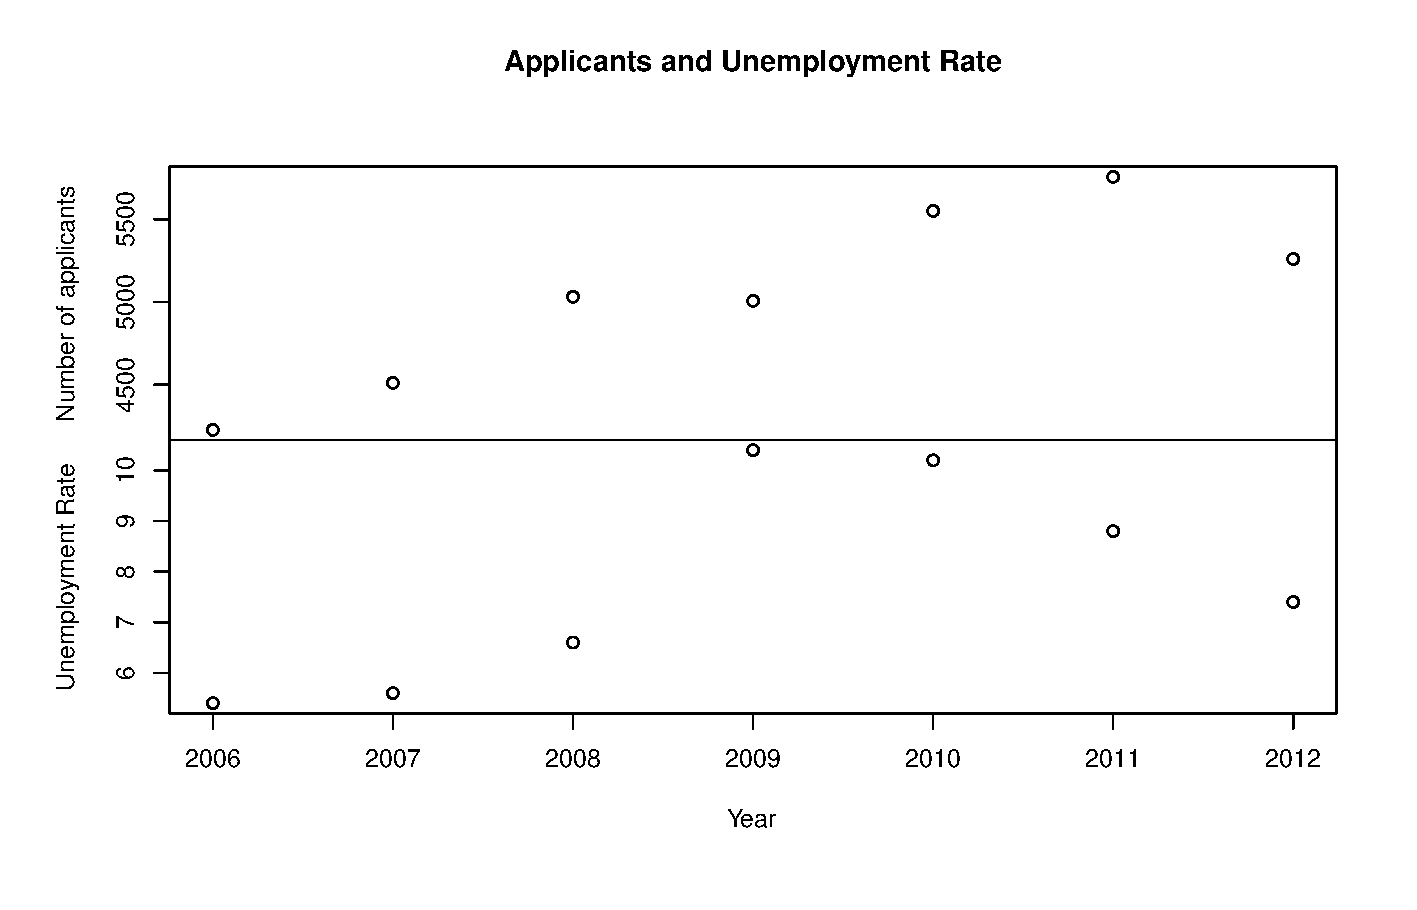
\includegraphics[scale=0.65]{pic/applicant_unmployment.eps}
 \caption{Applicants vs Unemployment Rate}
\end{figure}


\chapter{Appendix B: Piecewise Regression for Scholarship}  \label{AppB}

\begin{figure}[ht]
   \centering
 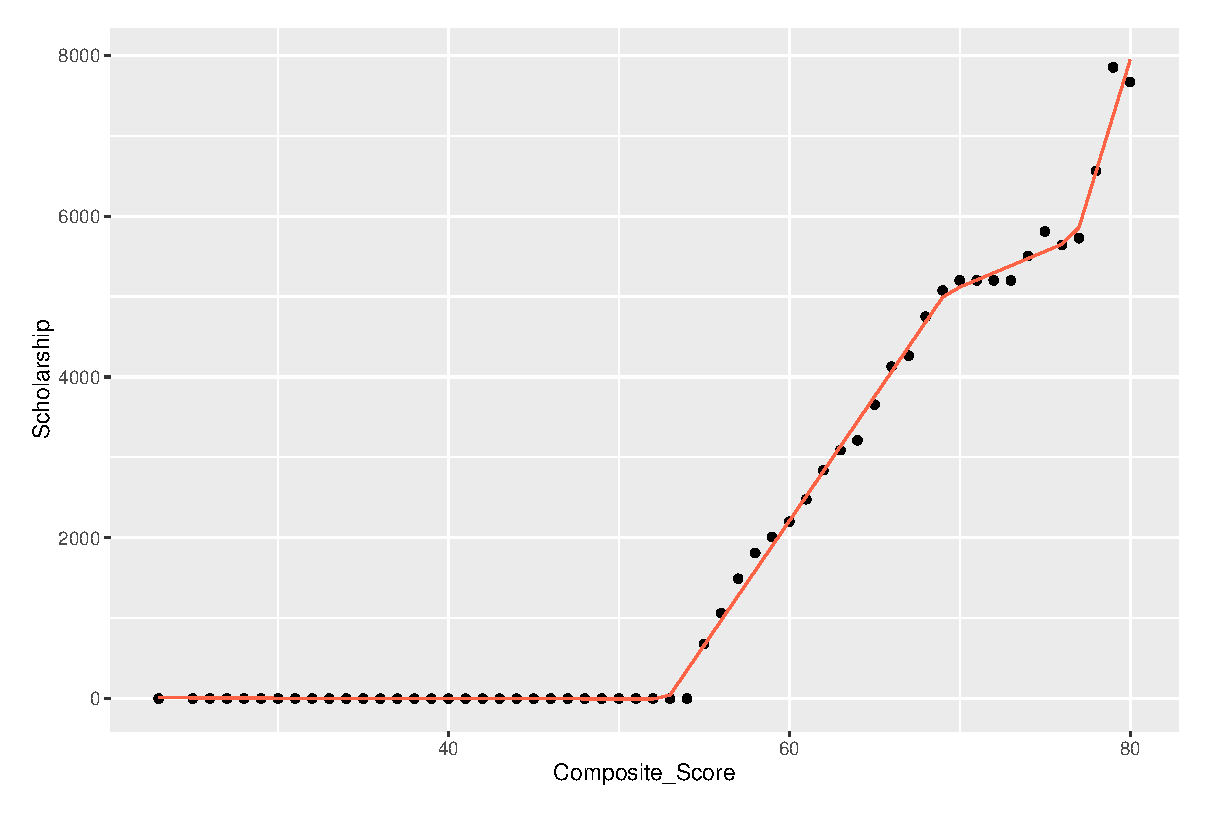
\includegraphics[scale=0.75]{pic/PieceWiseRegression.eps}
 \caption{PieceWise Linear Regression Result and the Original Results}
 \label{PieceWisePolicy}
\end{figure}




\begin{comment}
The response variables in the enrollment and graduation models are:
\begin{itemize}
	\item MATRICULATION. Whether the applicant enrolled or not.
	\item DEGREE.AWARDED. Whether the enrolled applicant graduated or not.
\end{itemize}

The variables represent applicant's academic performance in the model include: 
\begin{itemize}
\item GPA. The high school GPA of the applicant. The range of the GPA is 0.5 to
5. Some high school students take AP or college classes so that the GPA is
larger than 4.0.
\item  ACT. The highest ACT composite score that applicant reported. Applicant
only submit the highest ACT composite score. For student who took SAT, the
score was converted to ACT according to \citep{ACTSAT}.
\item HS.Percentile, ranging from 1 to 100, the applicant's percentile from the
high school, which is an easy way to represent applicant's standing at
graduation relative to other graduate.
\end{itemize}.    




The variables related to applicant's financial status include:
\begin{itemize}
\item TUITION. The amount of tuition that a applicant pays before the deduction
of any types of aids. Since this study does not include the out-of-state
applicants, the tuition are equal for all the applicants.
\item Family Effective Contribution (EFC). This variable is used to get the
Pell Grant information.
\item Pell Grant. The Pell Grant is converted from EFC, which followed by the
metric got from \citep{EFC_Pell}. There are 8560 applicants who did not fill
the EFC information in the data. I assumed these applicants knew that they did
qualify any Pell Grant, so that the NAs were converted to the lowest EFC which
does not qualify any Pell Grant.
\item SCHOLARSHIP. The amount amount of money applicant promised in the
enrollment stage.
\item TOTAL.FREE.MONEY. This variable is calculated as SCHOLARSHIP + PELL
GRANT. It represents that all the aids that one applicant got.
\item OUT.OF.POCKET. It is calculated as TUITION - Total.FREE.MONEY. This
indicates how much money does one applicant needs to pay.
\item UNEMPLOYMENT.INDEX. The school year Ohio unemployment rate was added to
reflect the overall economy. It is known that college is the safe harbor when
economy underperforms \citep{barr2015out}.
\end{itemize}

The personal information variables include:
\begin{itemize}
	\item GENDER. Applicant's gender.
\item HS.COUNTY.TIER. Since Wright State University is a commuter school, the
distance between home and campus could be an important factor. This variable
relates to the distance from the county in which the applicant lived, to Wright
State. There were six tiers in all, as well as “Out of State/Unknown”
subcategory. Tier 1 included students who lived in: Clark, Greene, Miami and
Montgomery counties. Tier 2: Butler, Champaign, Clinton, Darke, Preble and
Warren counties. Tier 3: included Auglaize, Mercer and Shelby counties. Tier 4
included Franklin, and Hamilton counties. Tier 5 was northern Ohio counties.
And Tier 6 was all other Ohio counties. As you can see, Tier 1 includes the
counties closest to Wright State, and Tier 5, 6/Out of State include the
counties furthest from Wright State.
\item HS.DISTANCE. The numeric value of distance between high school and campus
are also added.

\item ETHNICITY. This variable has several different ethnicities:
BlackOrAfricanAmerican, White, Asian, Hispanic, TwoMore.
	\item APP.COLLEGE. The intended college of a applicant.
\end{itemize}

\end{comment}

%-----------------------------------------------------------------------
% Bibliography
%-----------------------------------------------------------------------
\clearpage \phantomsection %used to correctly anchor hyperlinks
\renewcommand\baselinestretch{1.5}
%\addcontentsline{toc}{chapter}{Bibliography}
%\bibliographystyle{apalike}
\bibliographystyle{plainnat}
\bibliography{shuai_cita}


\renewcommand\baselinestretch{1.25}

\end{document} 	

  